\subsection{Аналитическая механика}
	
	\subsubsection{Аннотация}

		Курс <<Аналитическая механика>> получил в основном положительные отзывы. Острых проблем с курсом не было выявлено.

		Лекции Фомичева А.В. получили крайне положительные отзывы, однако есть ряд недостатков. Студенты отметили, что темп лекций иногда становится слишком быстрым, что осложняет усвоение материала. Совет студентов и аспирантов ФРКТ просит передать эти сведения лектору.

        Семинаристы Амелькин Н.И., Ахлумади Махди Реза, Маштаков Я.В., Монахова У.В., Фомичев А.В. получили крайне положительные оценки от респондентов. Совет студентов и аспирантов ФРКТ предлагает поощрить перечисленных преподавателей.



	\subsubsection{Общий отзыв студентов о курсе}

		\begin{figure}[H]
			\centering
			\begin{subfigure}[b]{0.45\textwidth}
				\centering
				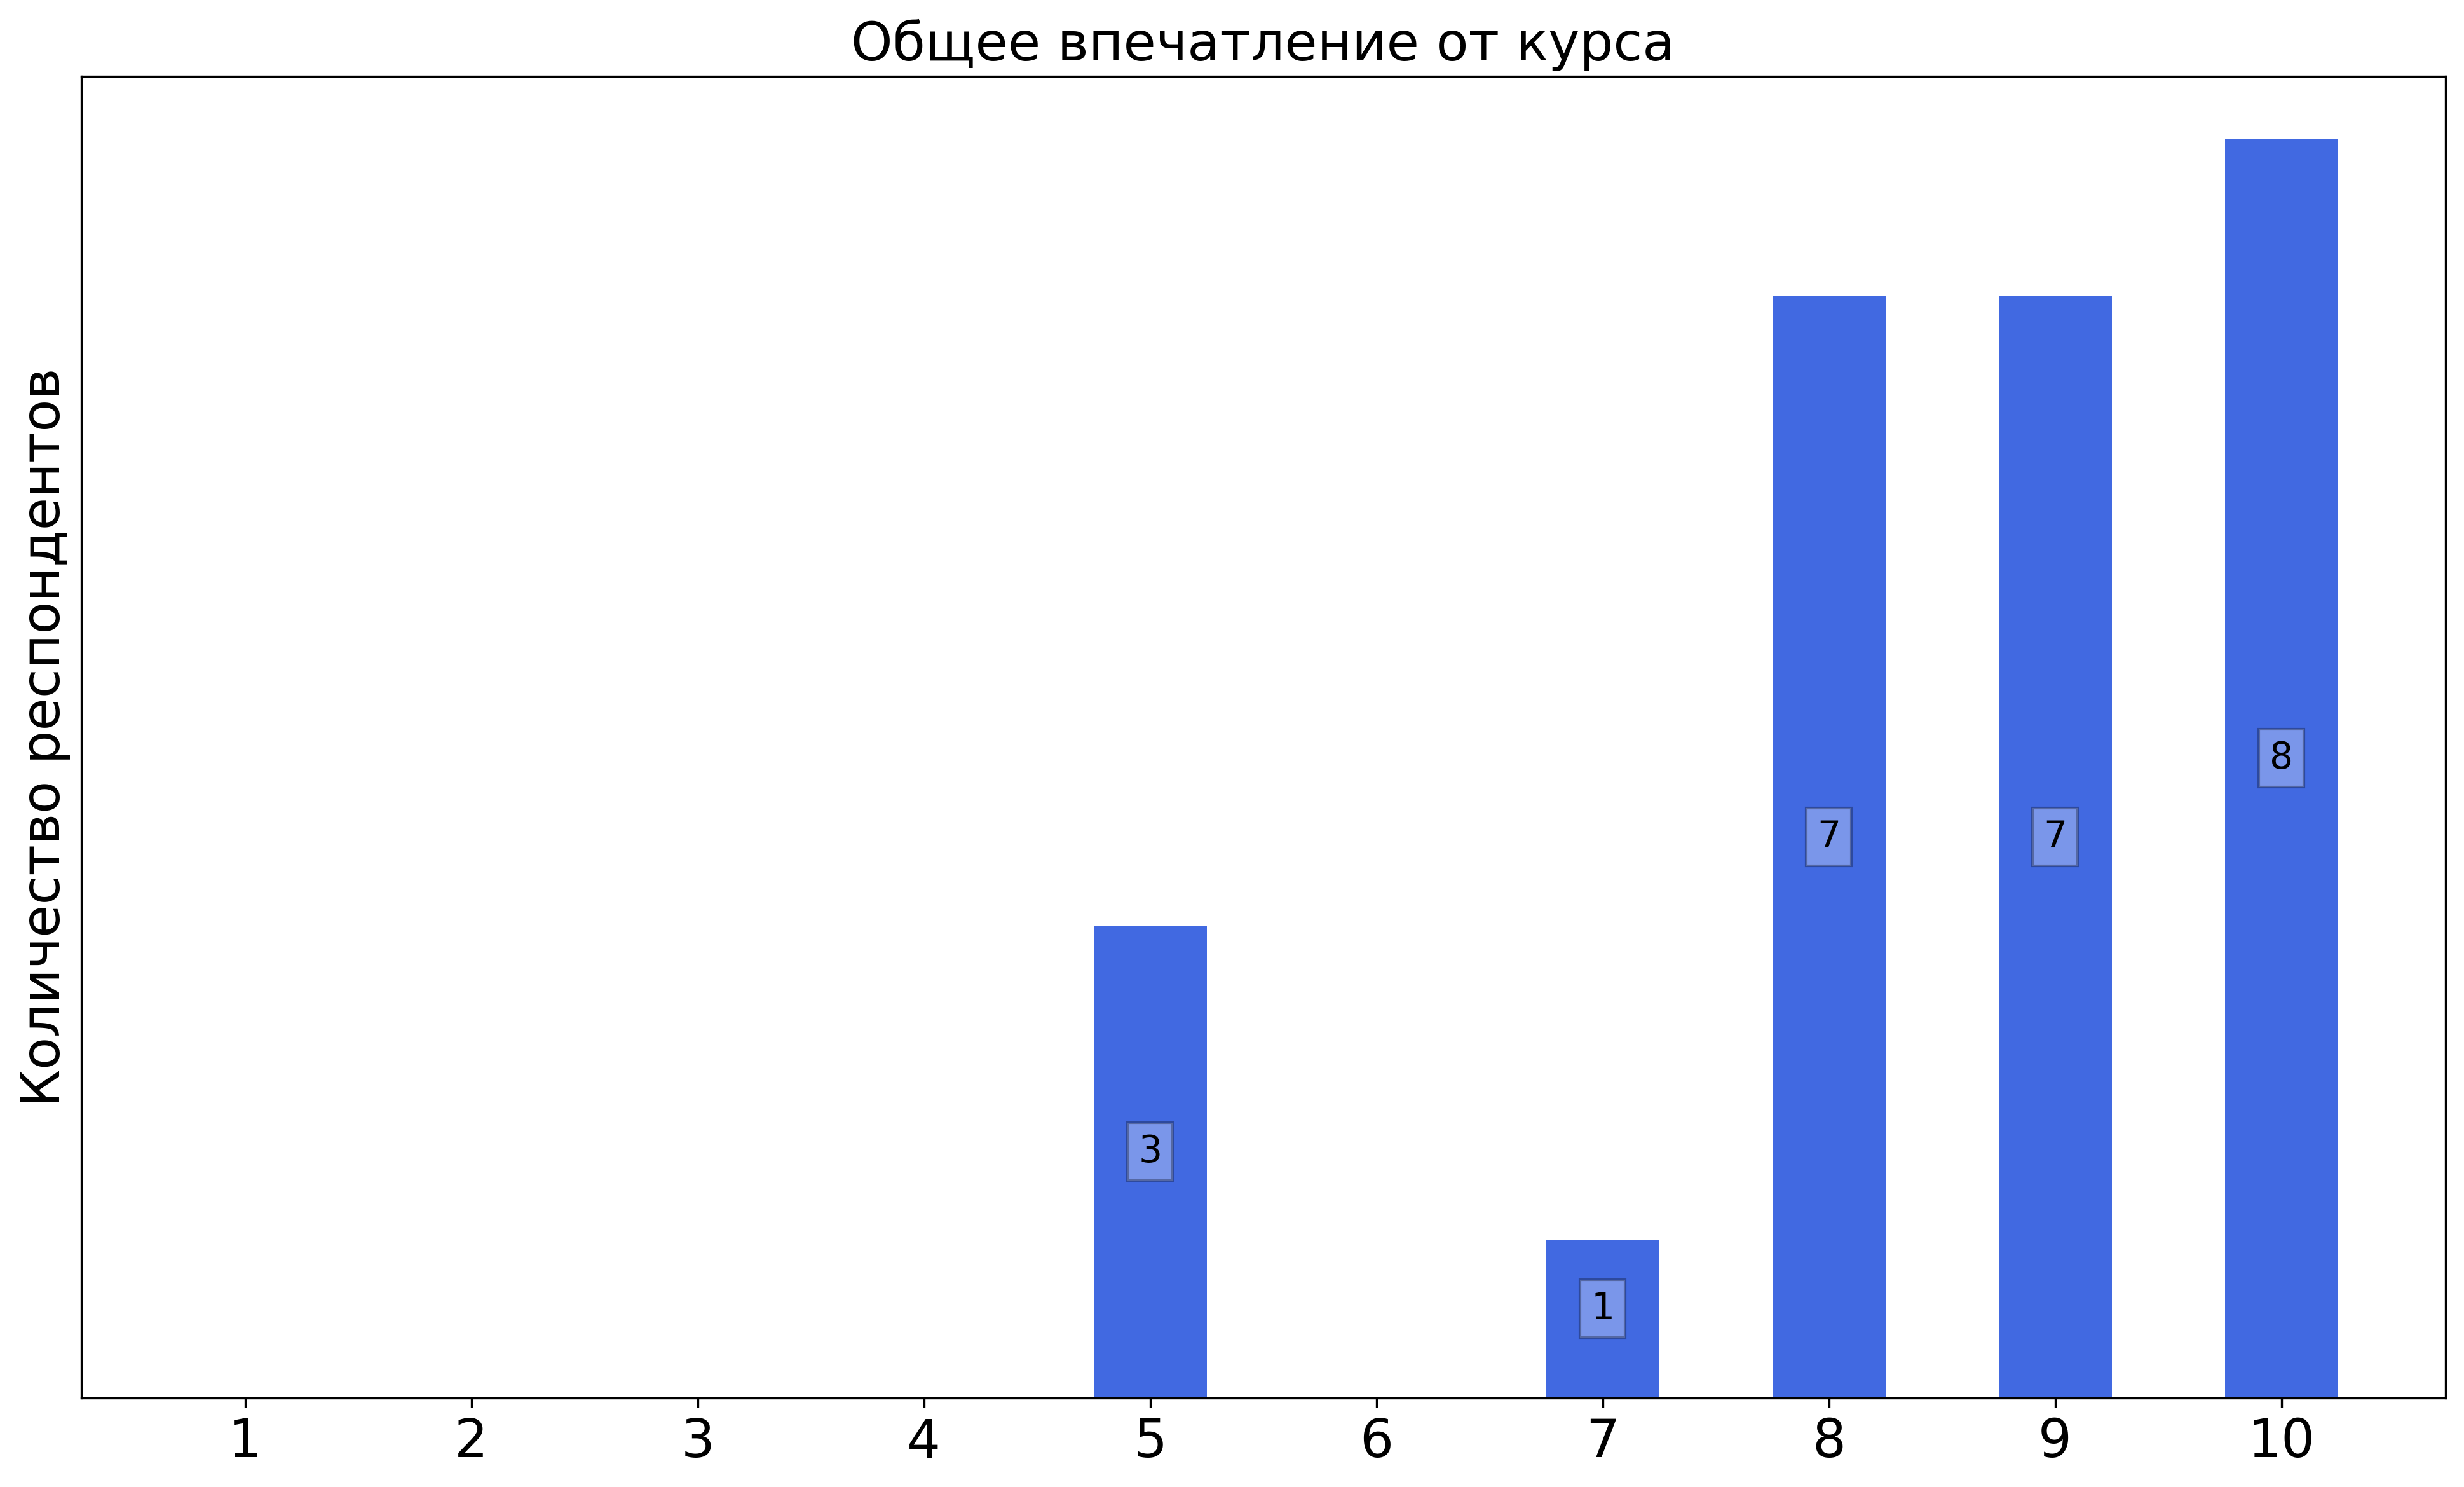
\includegraphics[width=\textwidth]{images/2 course/Аналитическая механика/general-0.png}
			\end{subfigure}
			\begin{subfigure}[b]{0.45\textwidth}
				\centering
				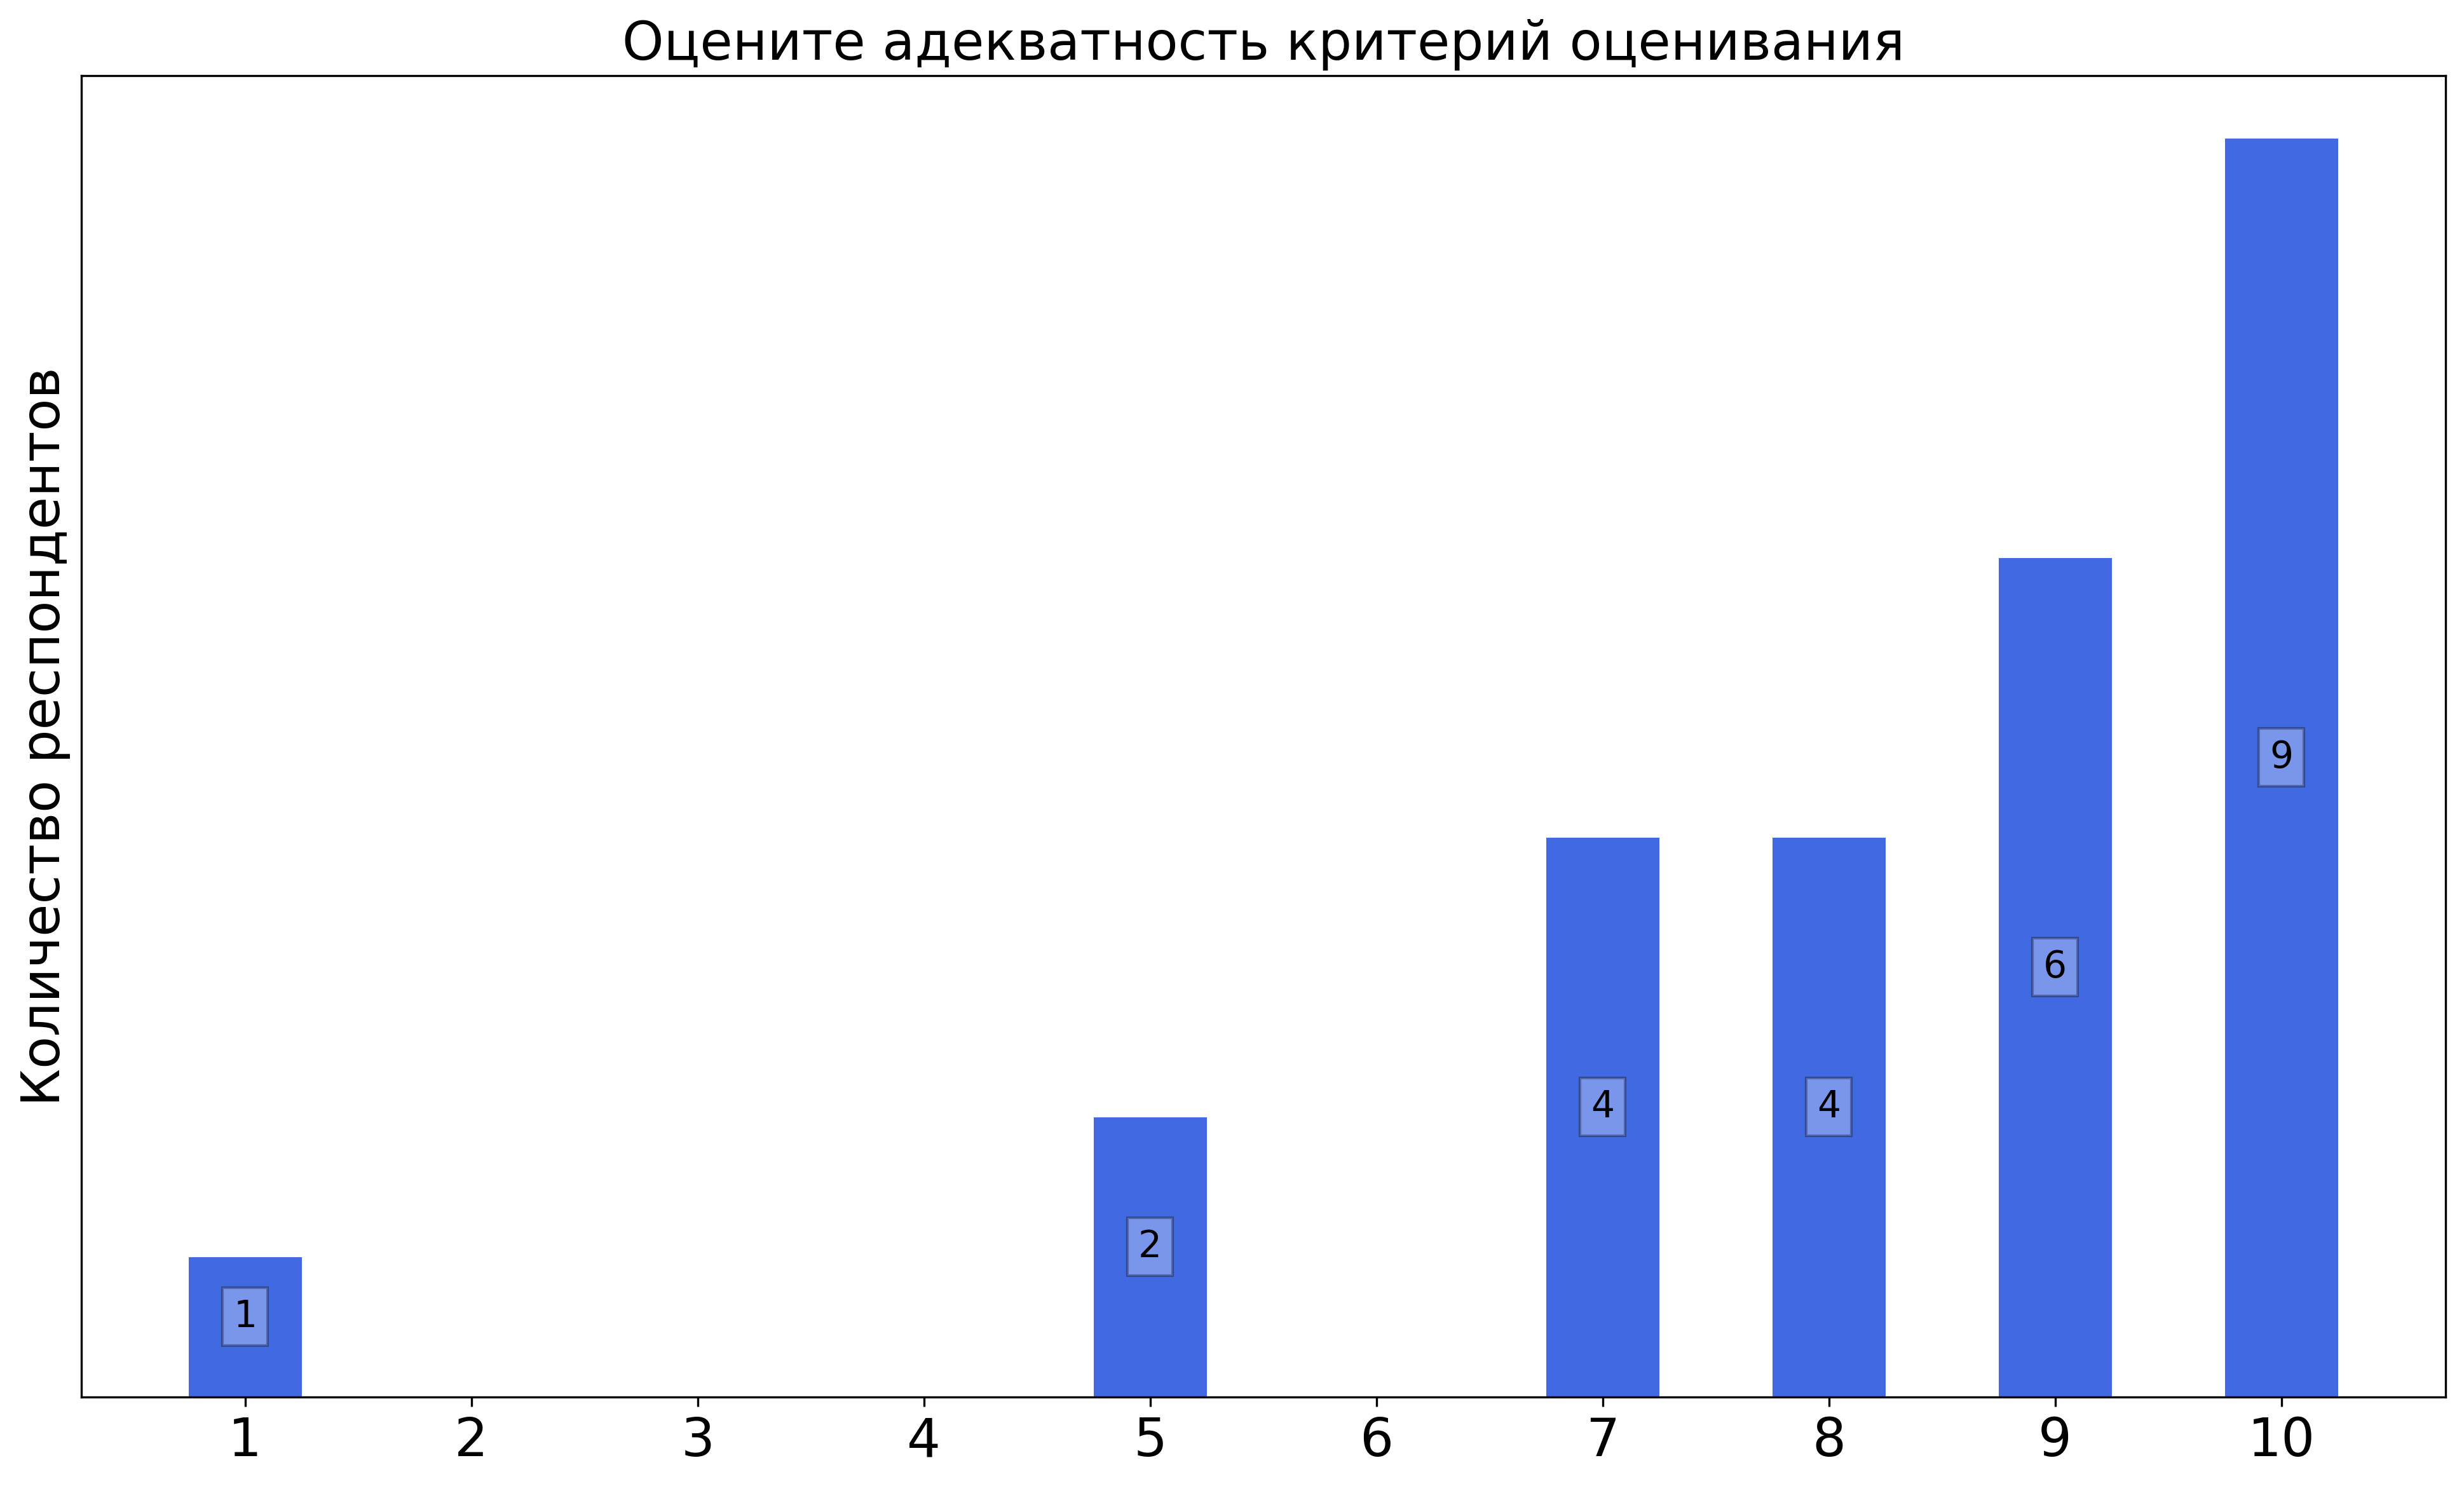
\includegraphics[width=\textwidth]{images/2 course/Аналитическая механика/general-1.png}
			\end{subfigure}	
		\end{figure}

	\subsubsection{Материалы, использумые респондентами при изучении курса}

		\begin{figure}[H]
			\centering
			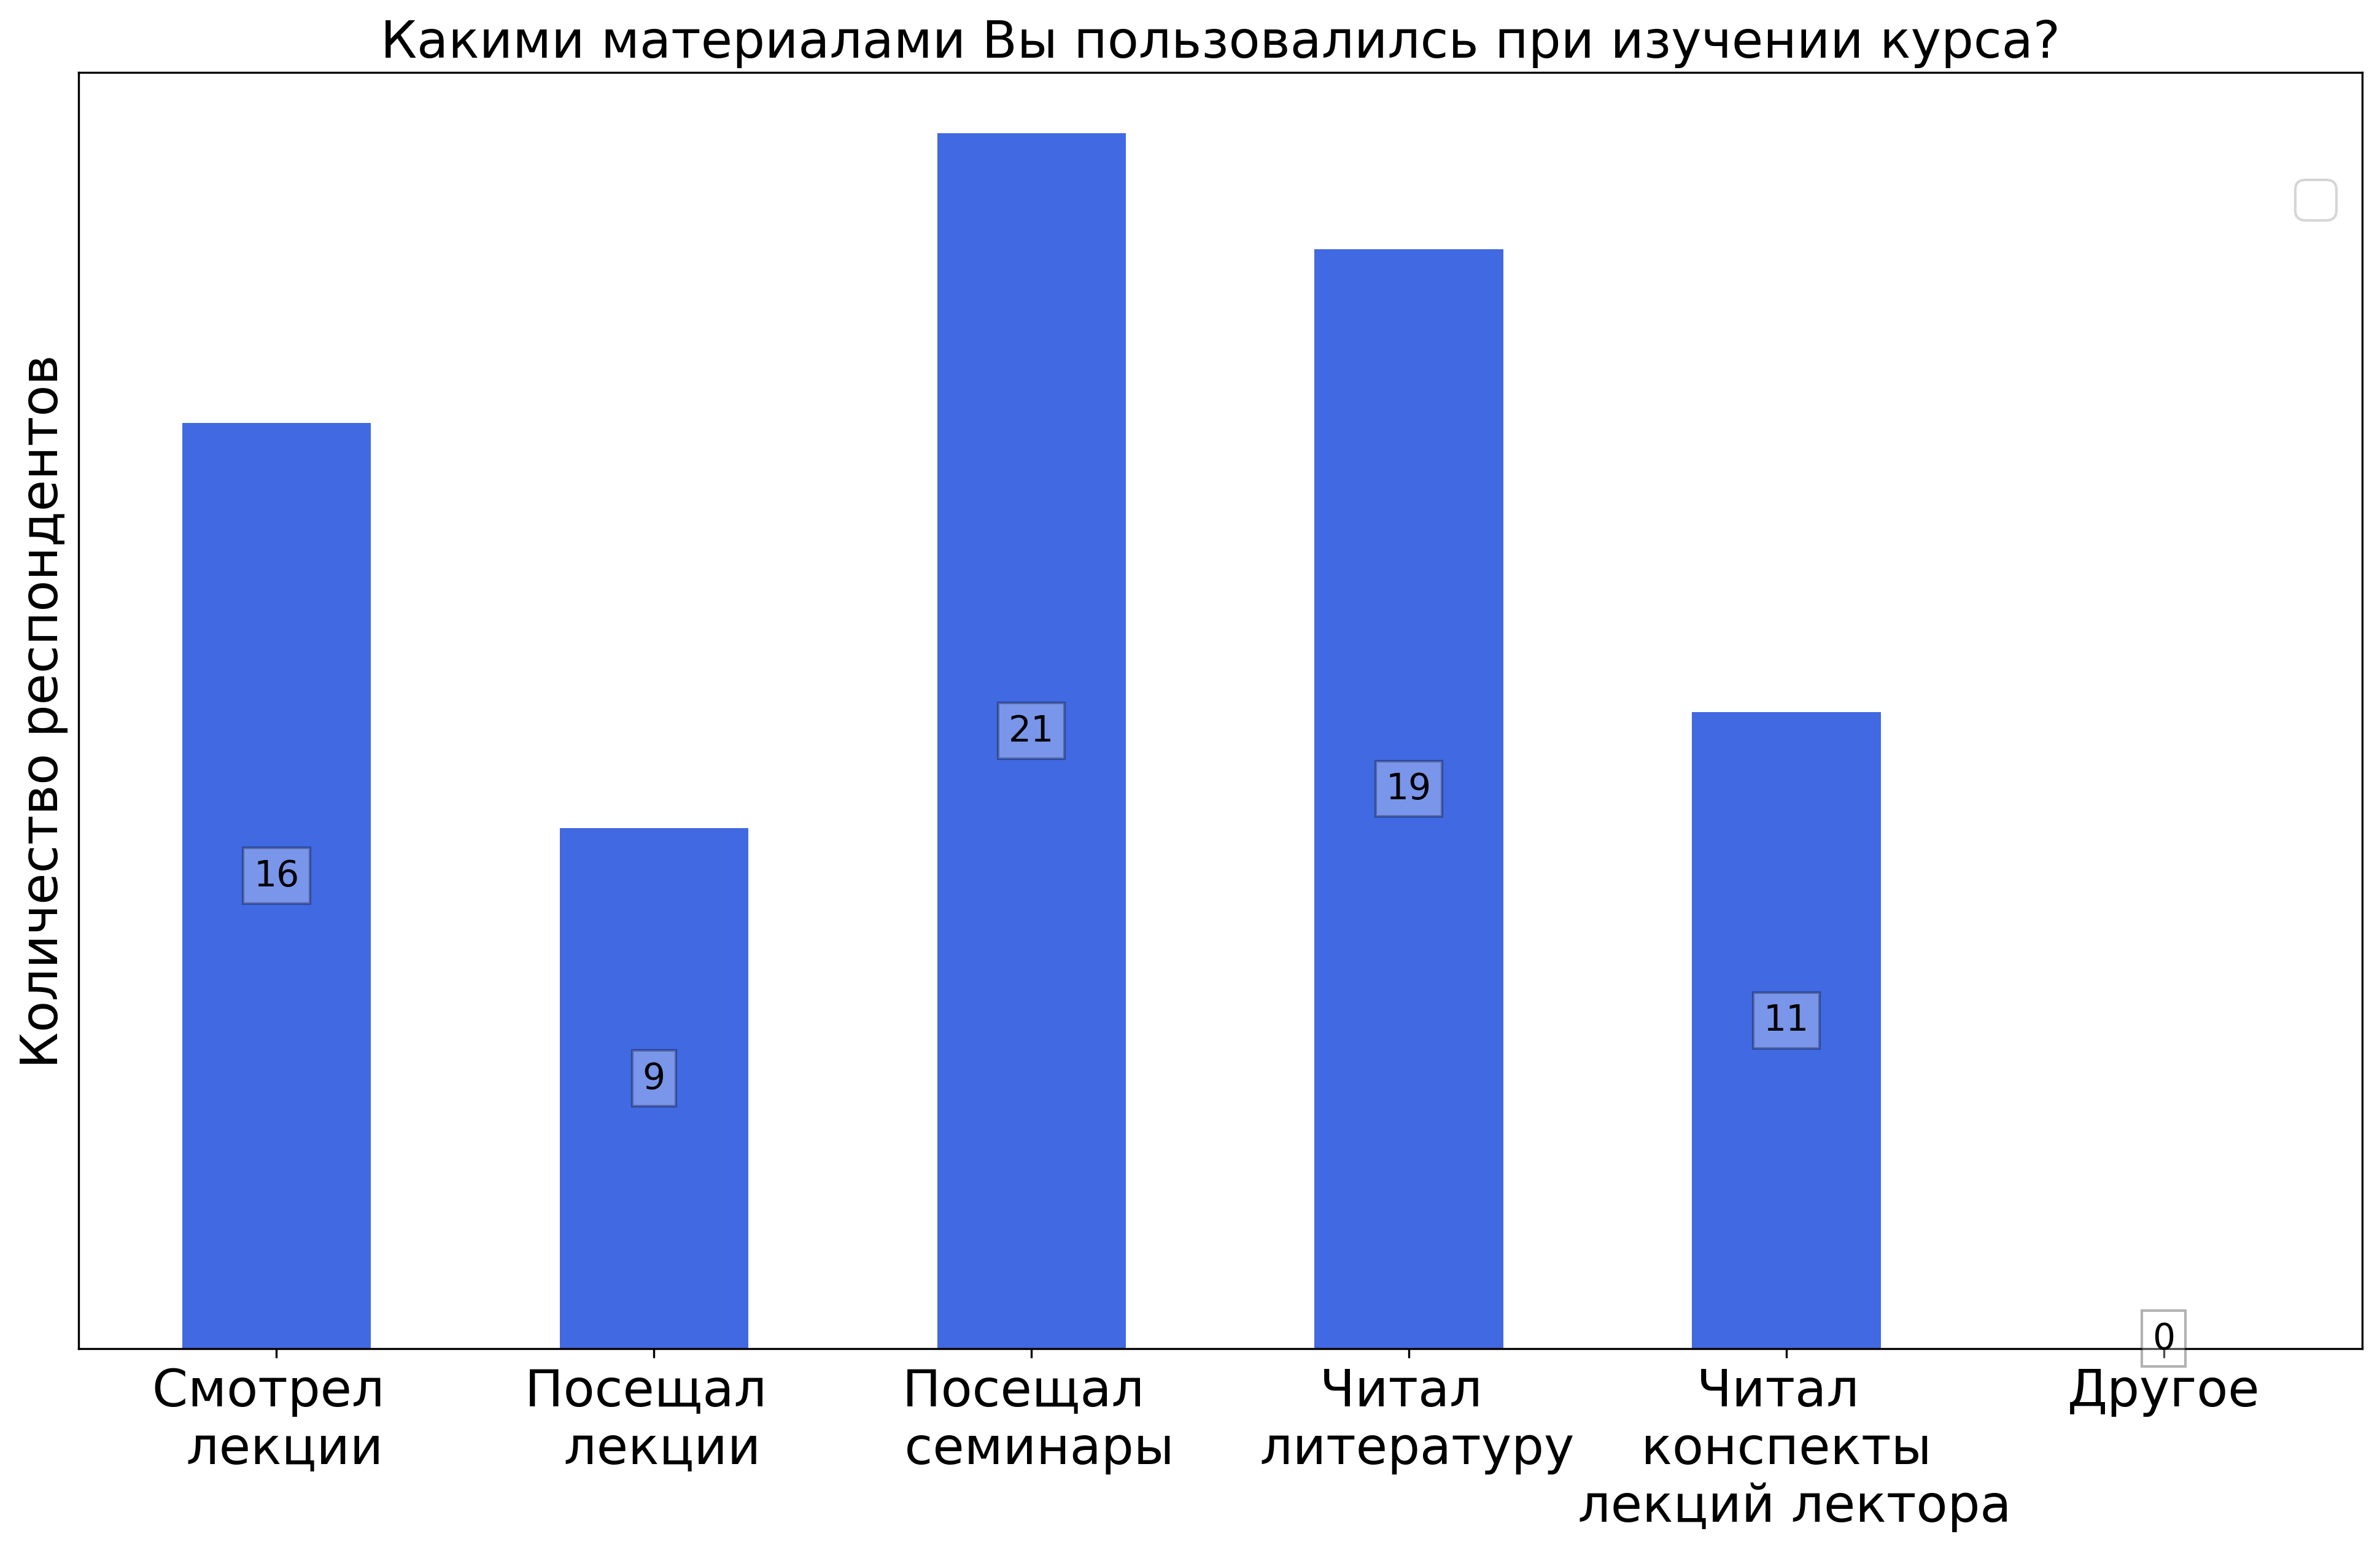
\includegraphics[width = 0.45\textwidth]{images/2 course/Аналитическая механика/materials.png}
		\end{figure}

	\subsubsection{Отзыв студентов о лекциях. Лектор: Фомичев А.В.}

		\begin{figure}[H]
			\centering
            \begin{subfigure}[b]{0.45\textwidth}
				\centering
				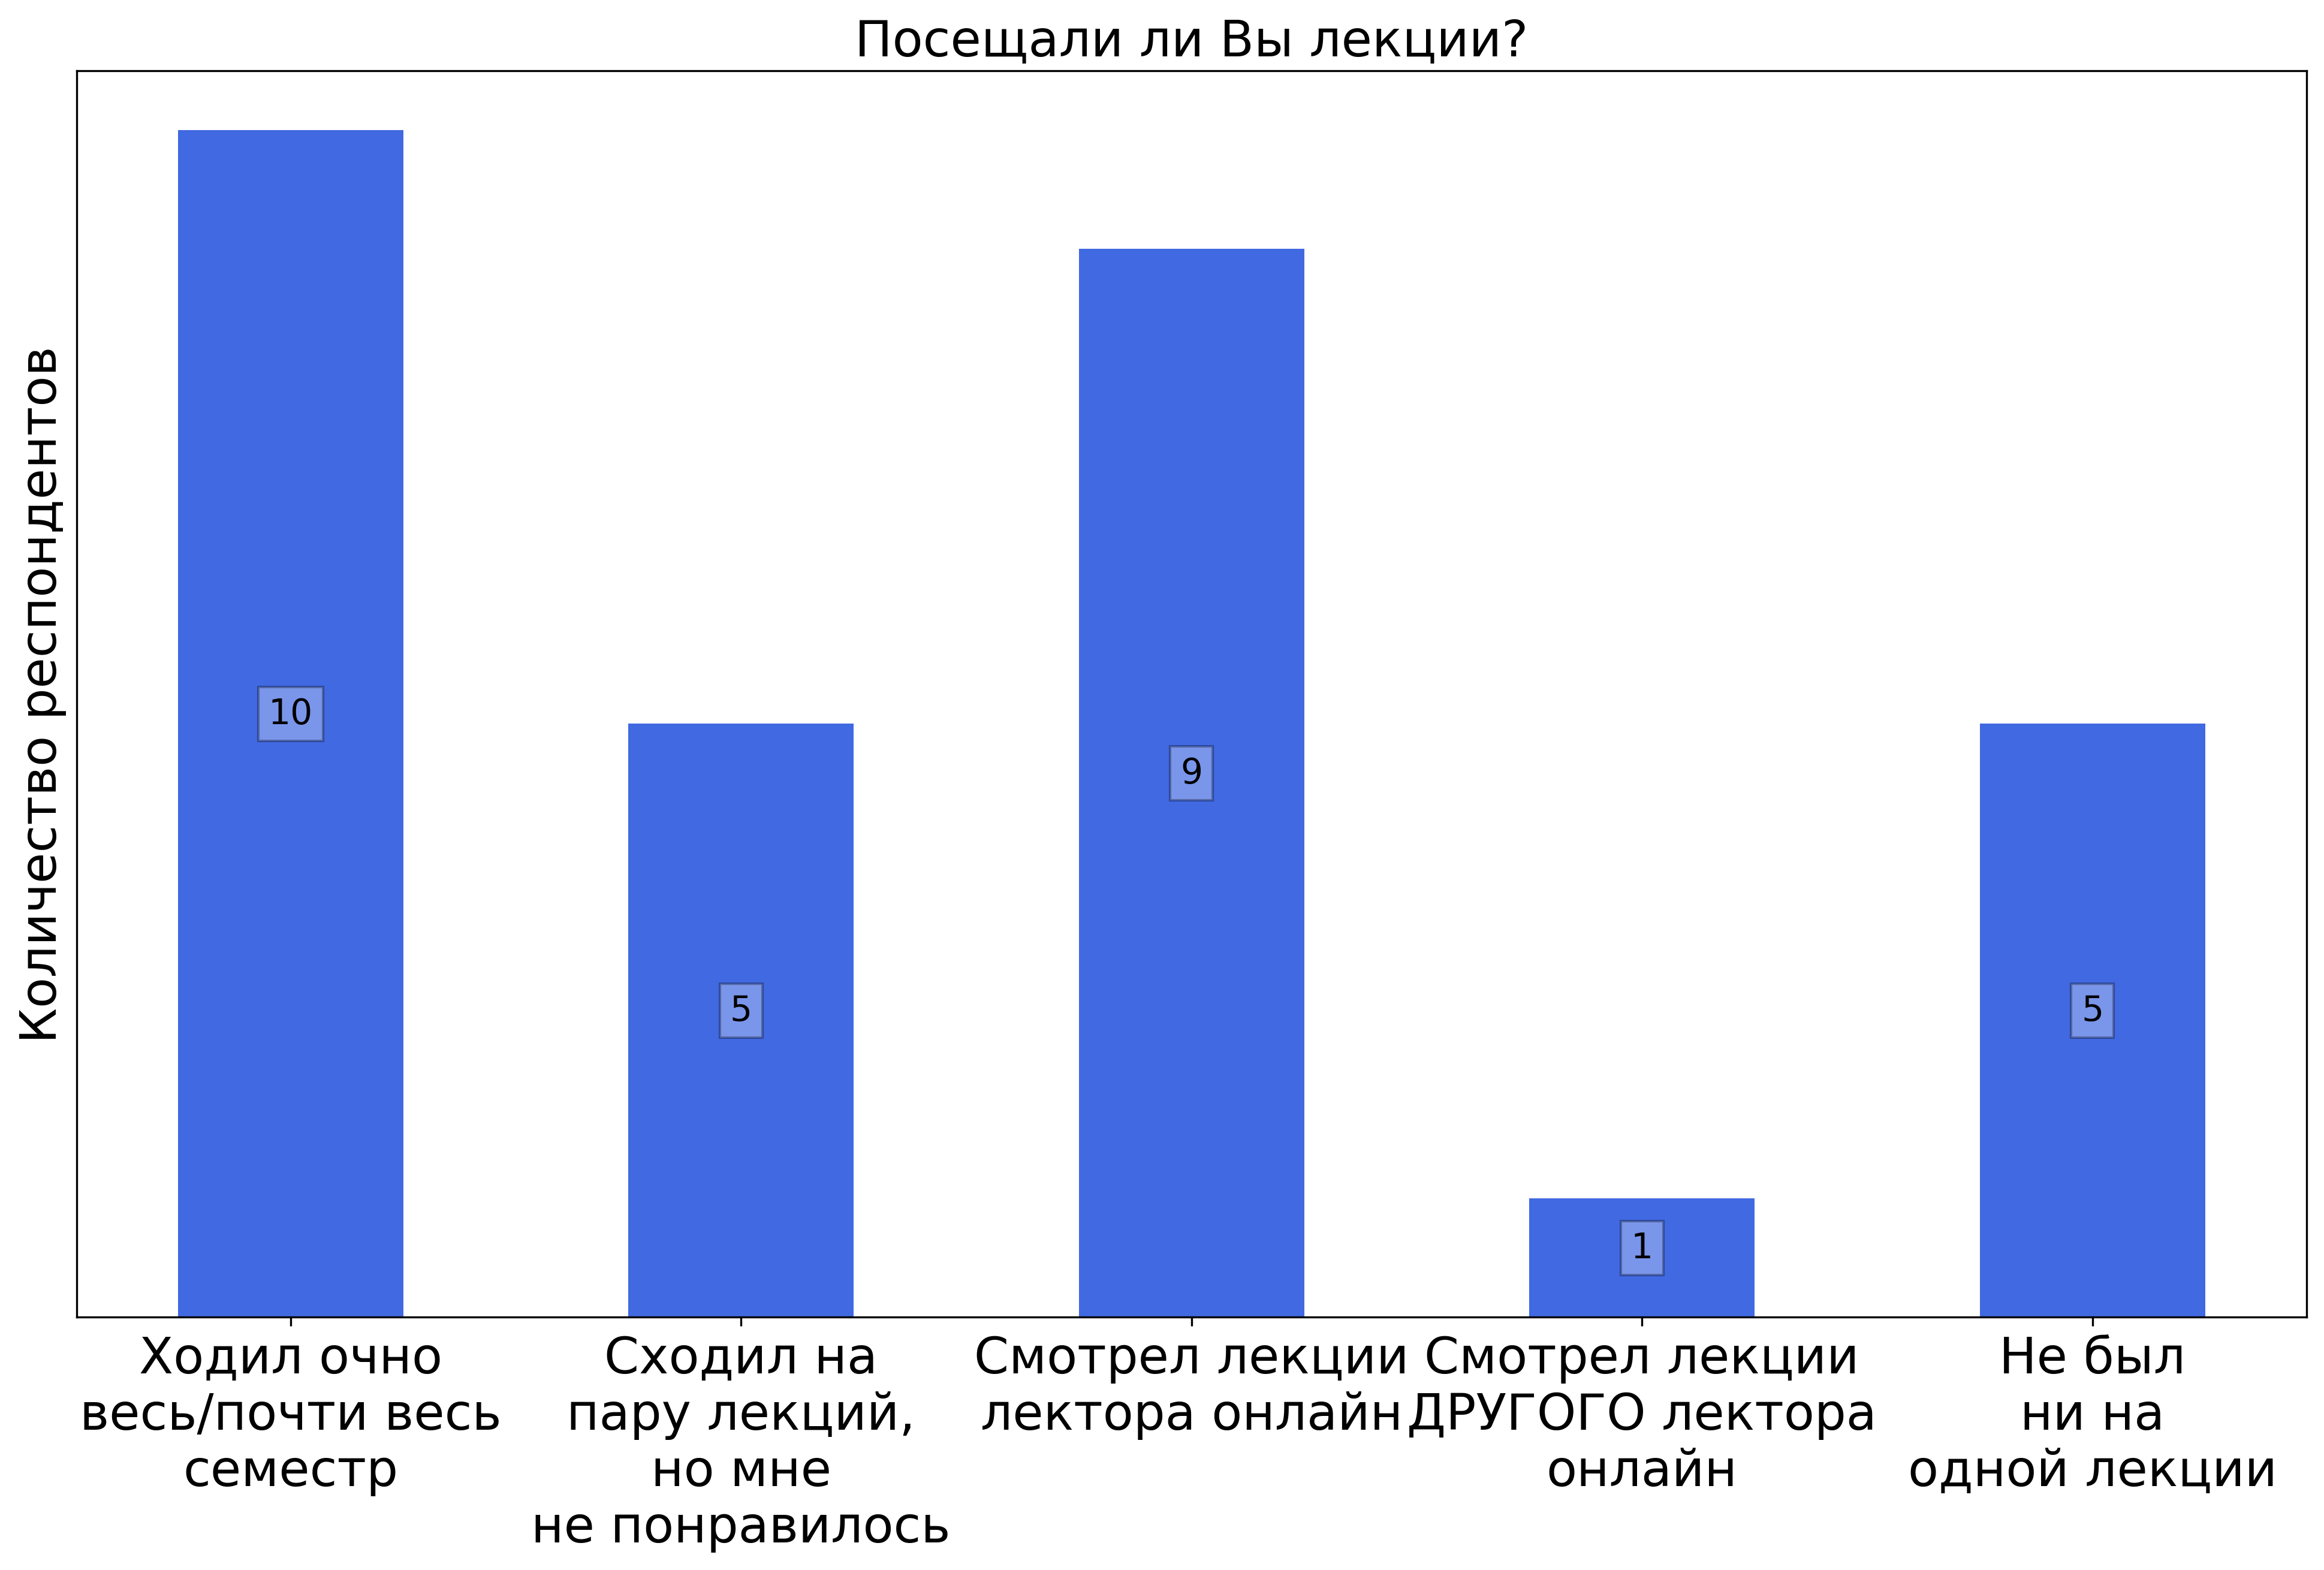
\includegraphics[width=\textwidth]{images/2 course/Аналитическая механика/lecturer-questions-Фомичев А.В.-0.png}
			\end{subfigure}
			\begin{subfigure}[b]{0.45\textwidth}
				\centering
				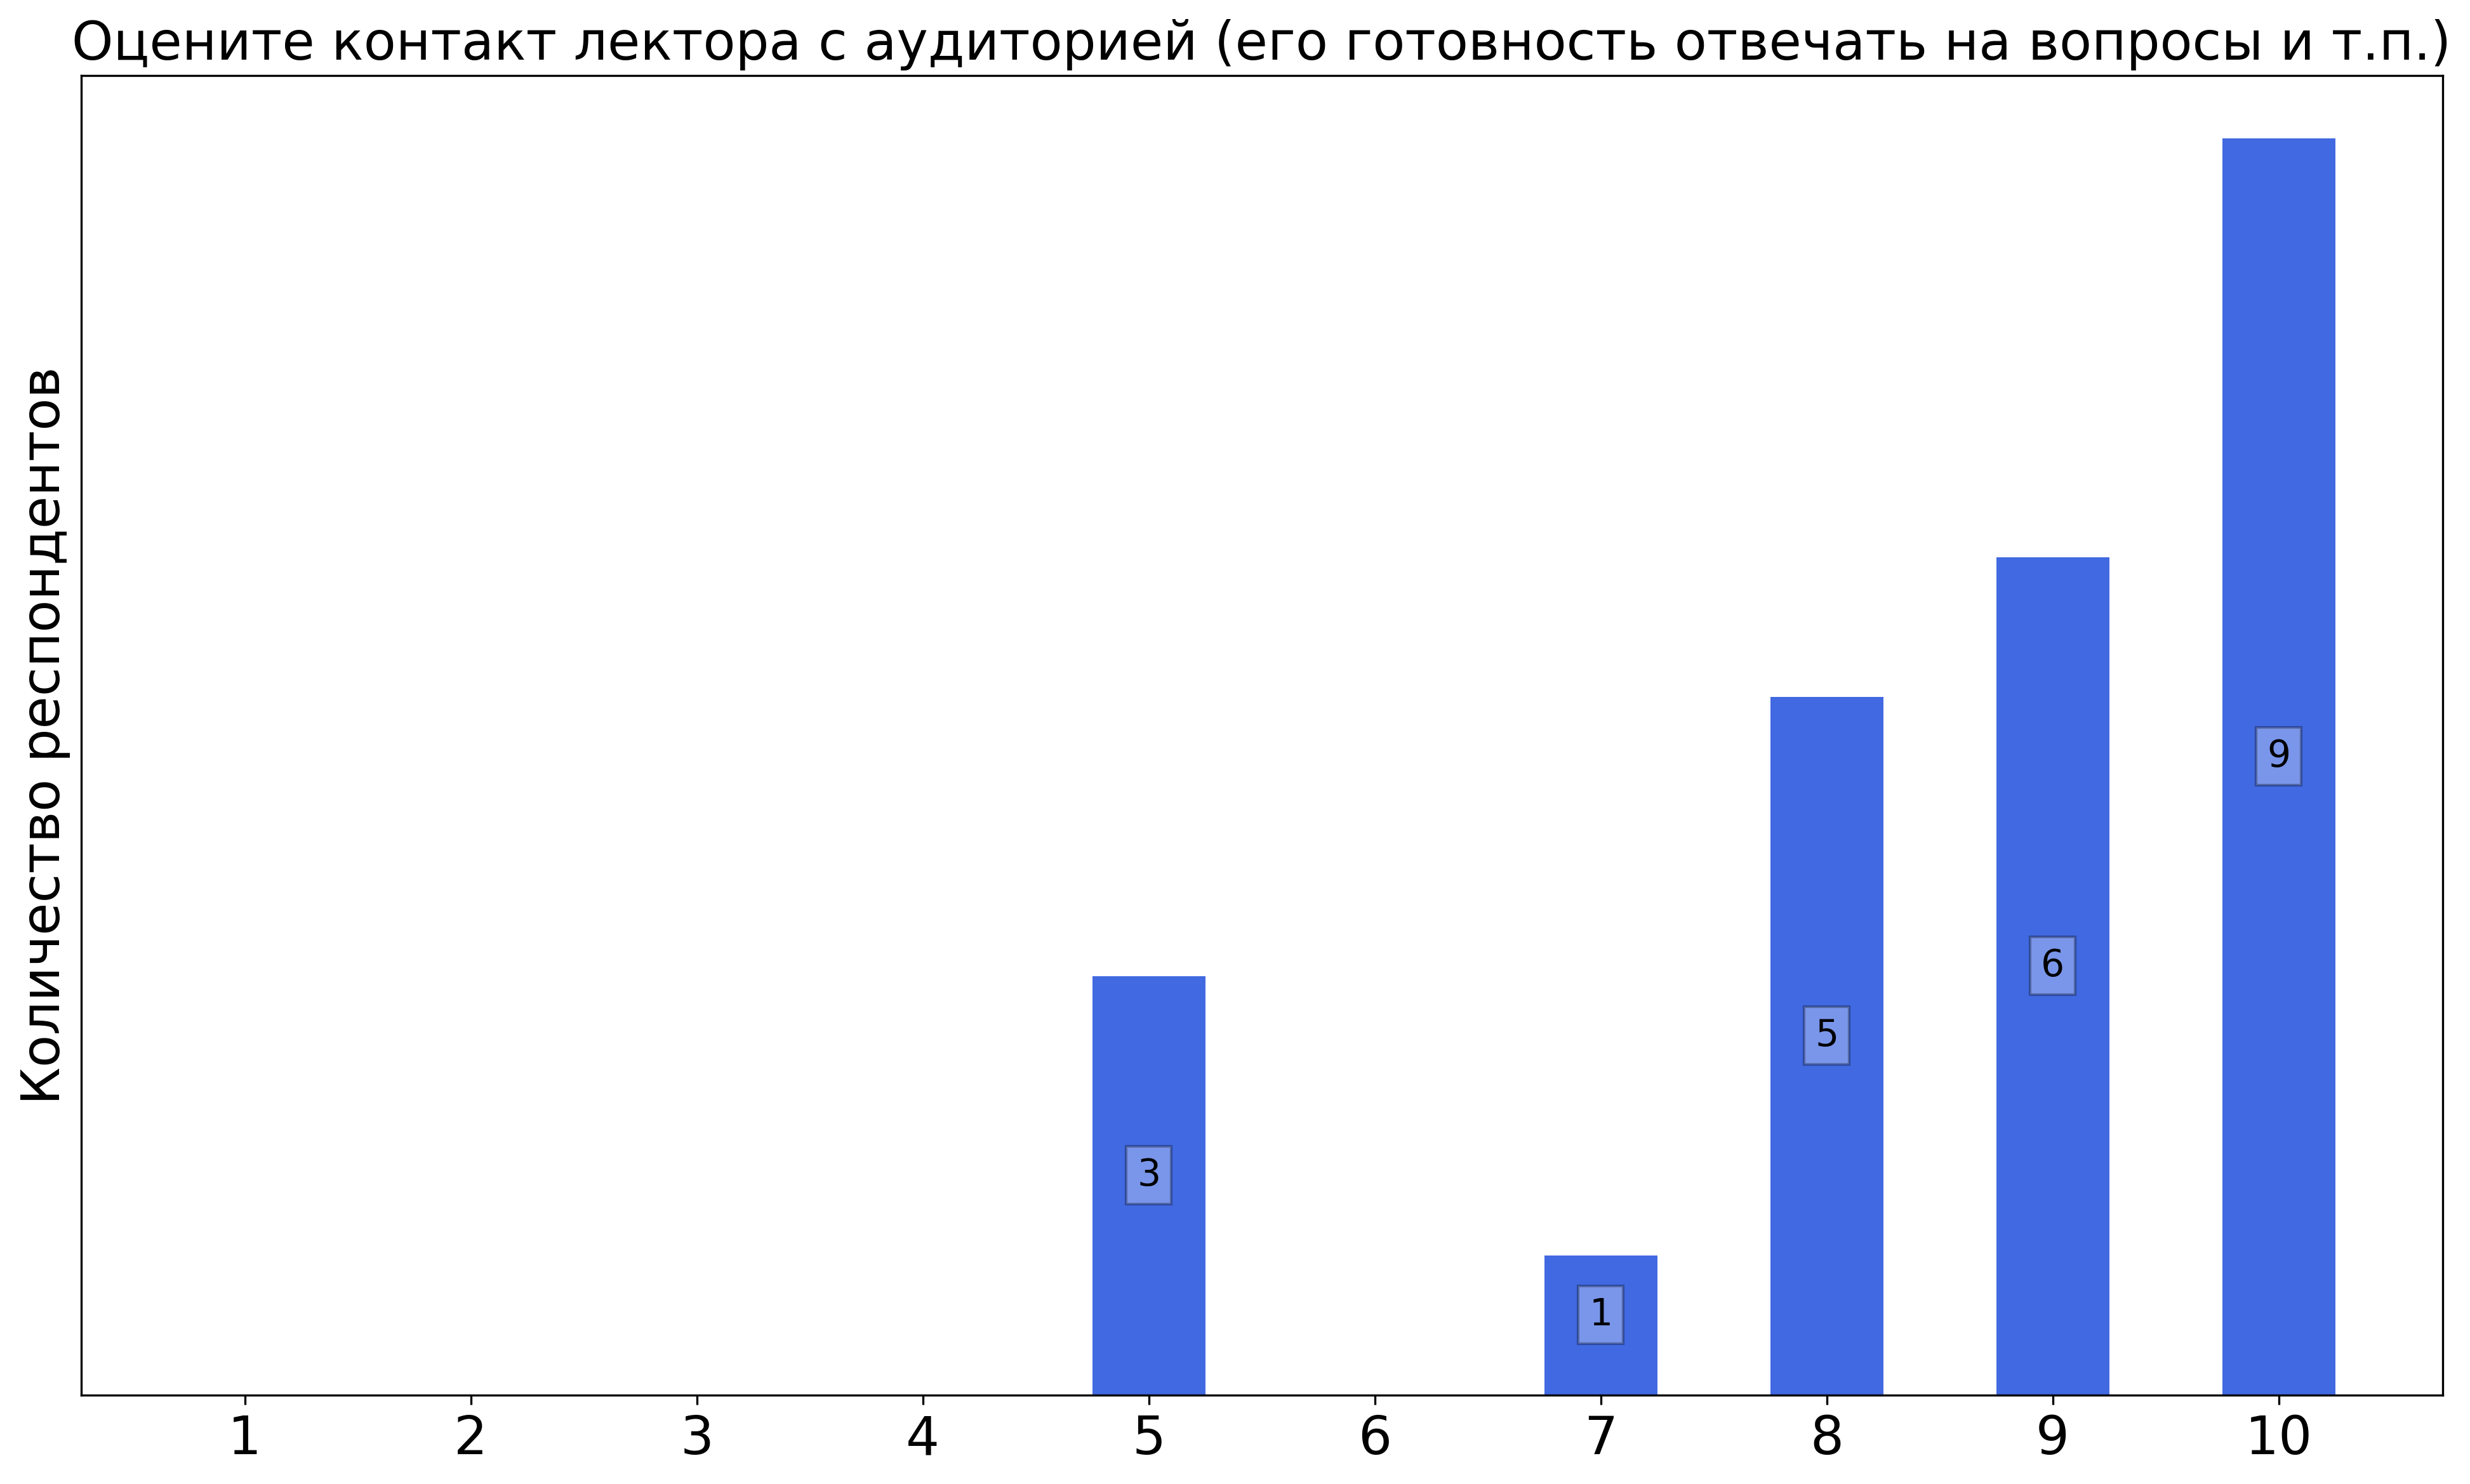
\includegraphics[width=\textwidth]{images/2 course/Аналитическая механика/lecturer-marks-Фомичев А.В.-0.png}
			\end{subfigure}
			\begin{subfigure}[b]{0.45\textwidth}
				\centering
				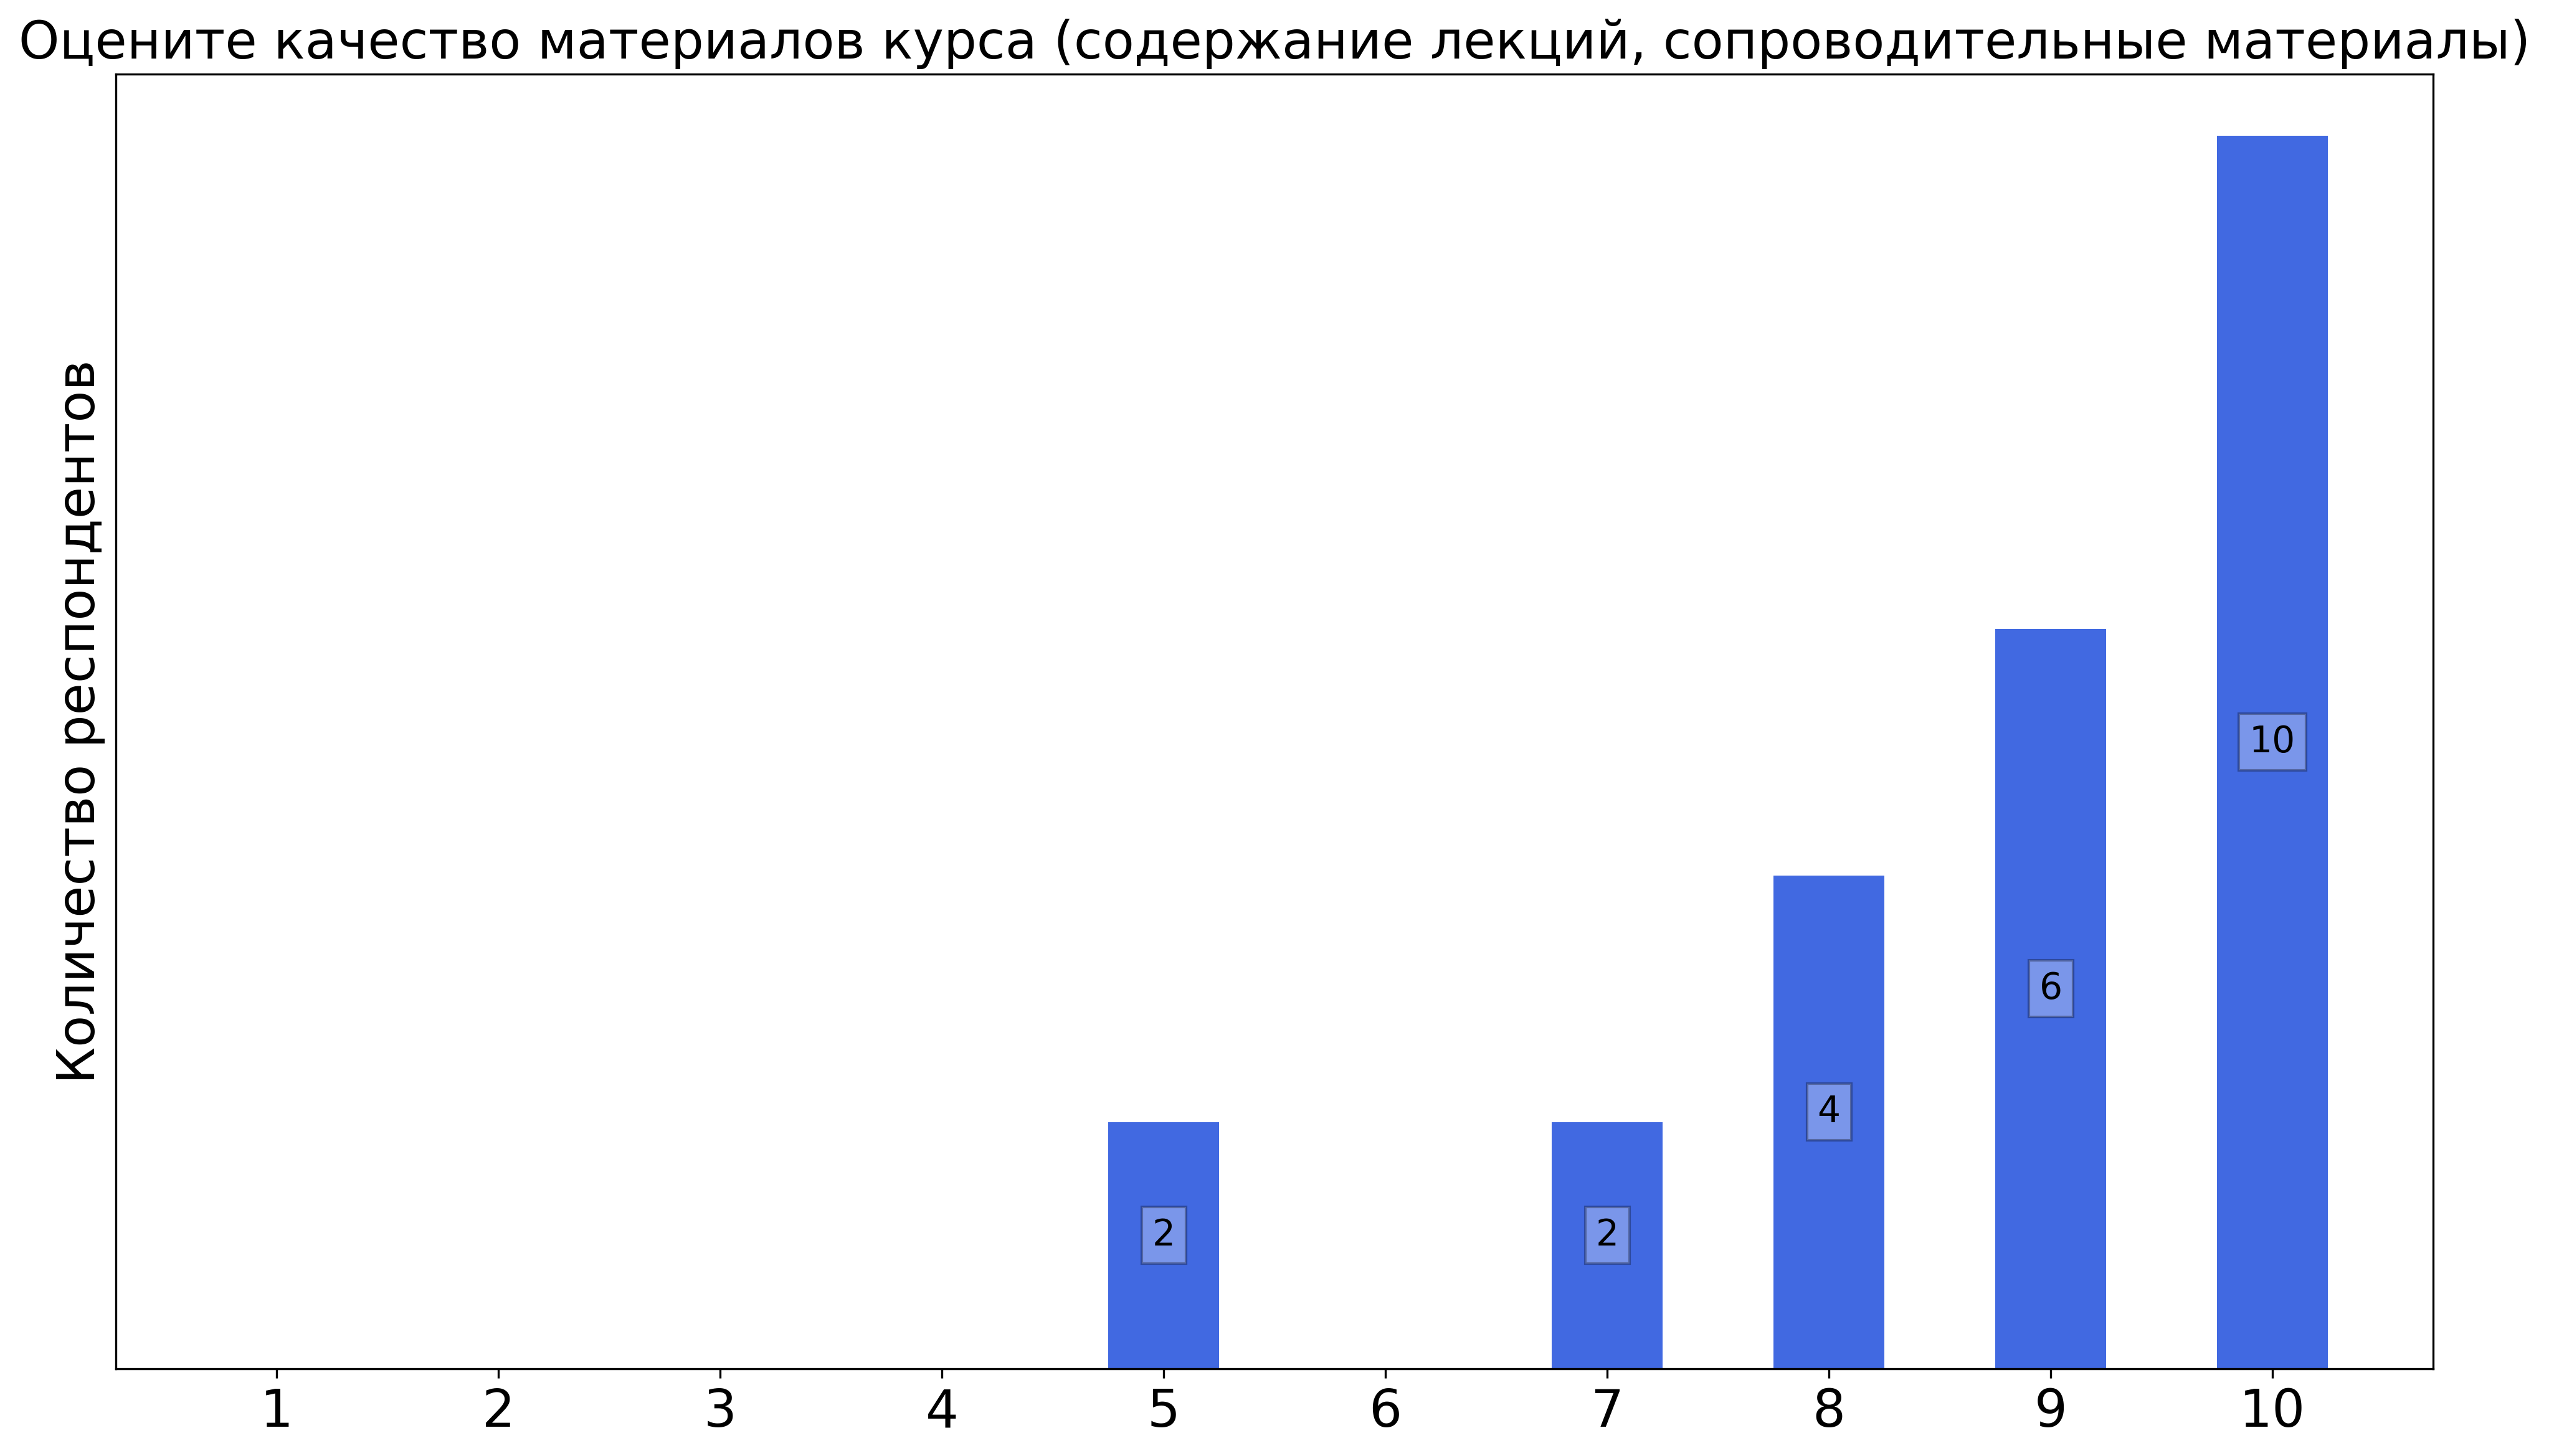
\includegraphics[width=\textwidth]{images/2 course/Аналитическая механика/lecturer-marks-Фомичев А.В.-1.png}
			\end{subfigure}
			\begin{subfigure}[b]{0.45\textwidth}
				\centering
				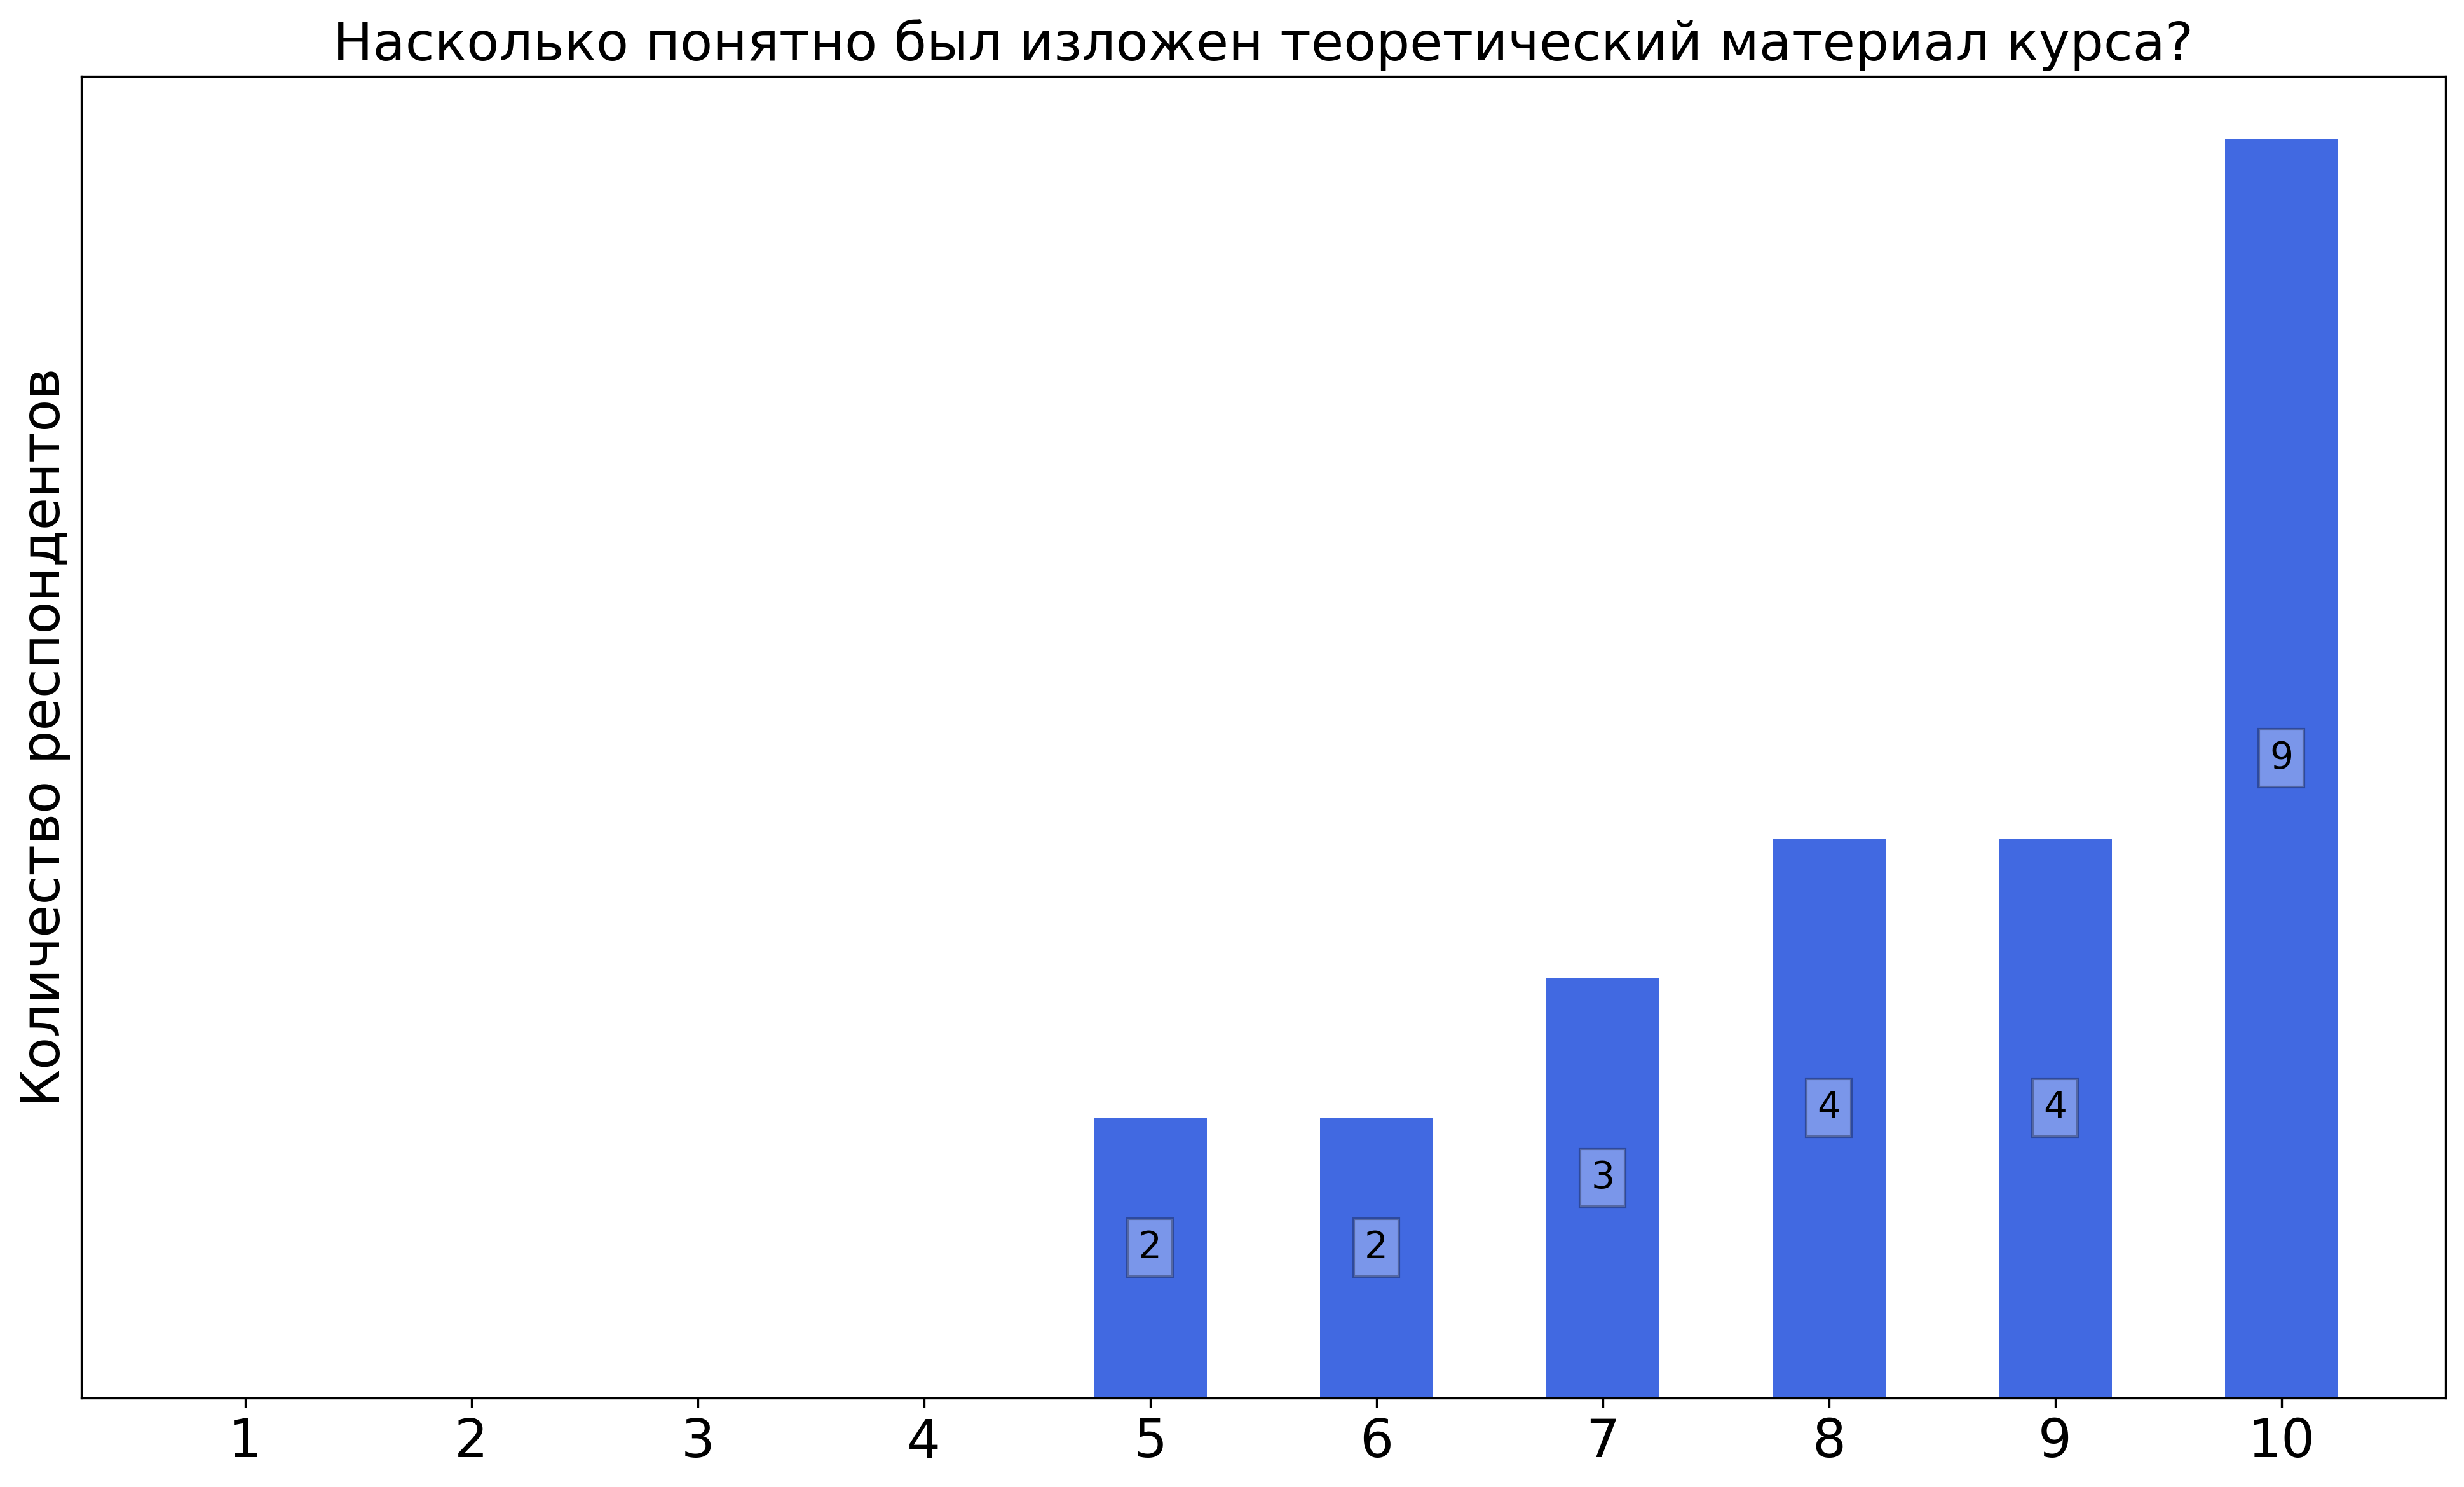
\includegraphics[width=\textwidth]{images/2 course/Аналитическая механика/lecturer-marks-Фомичев А.В.-2.png}
			\end{subfigure}	
			\begin{subfigure}[b]{0.45\textwidth}
				\centering
				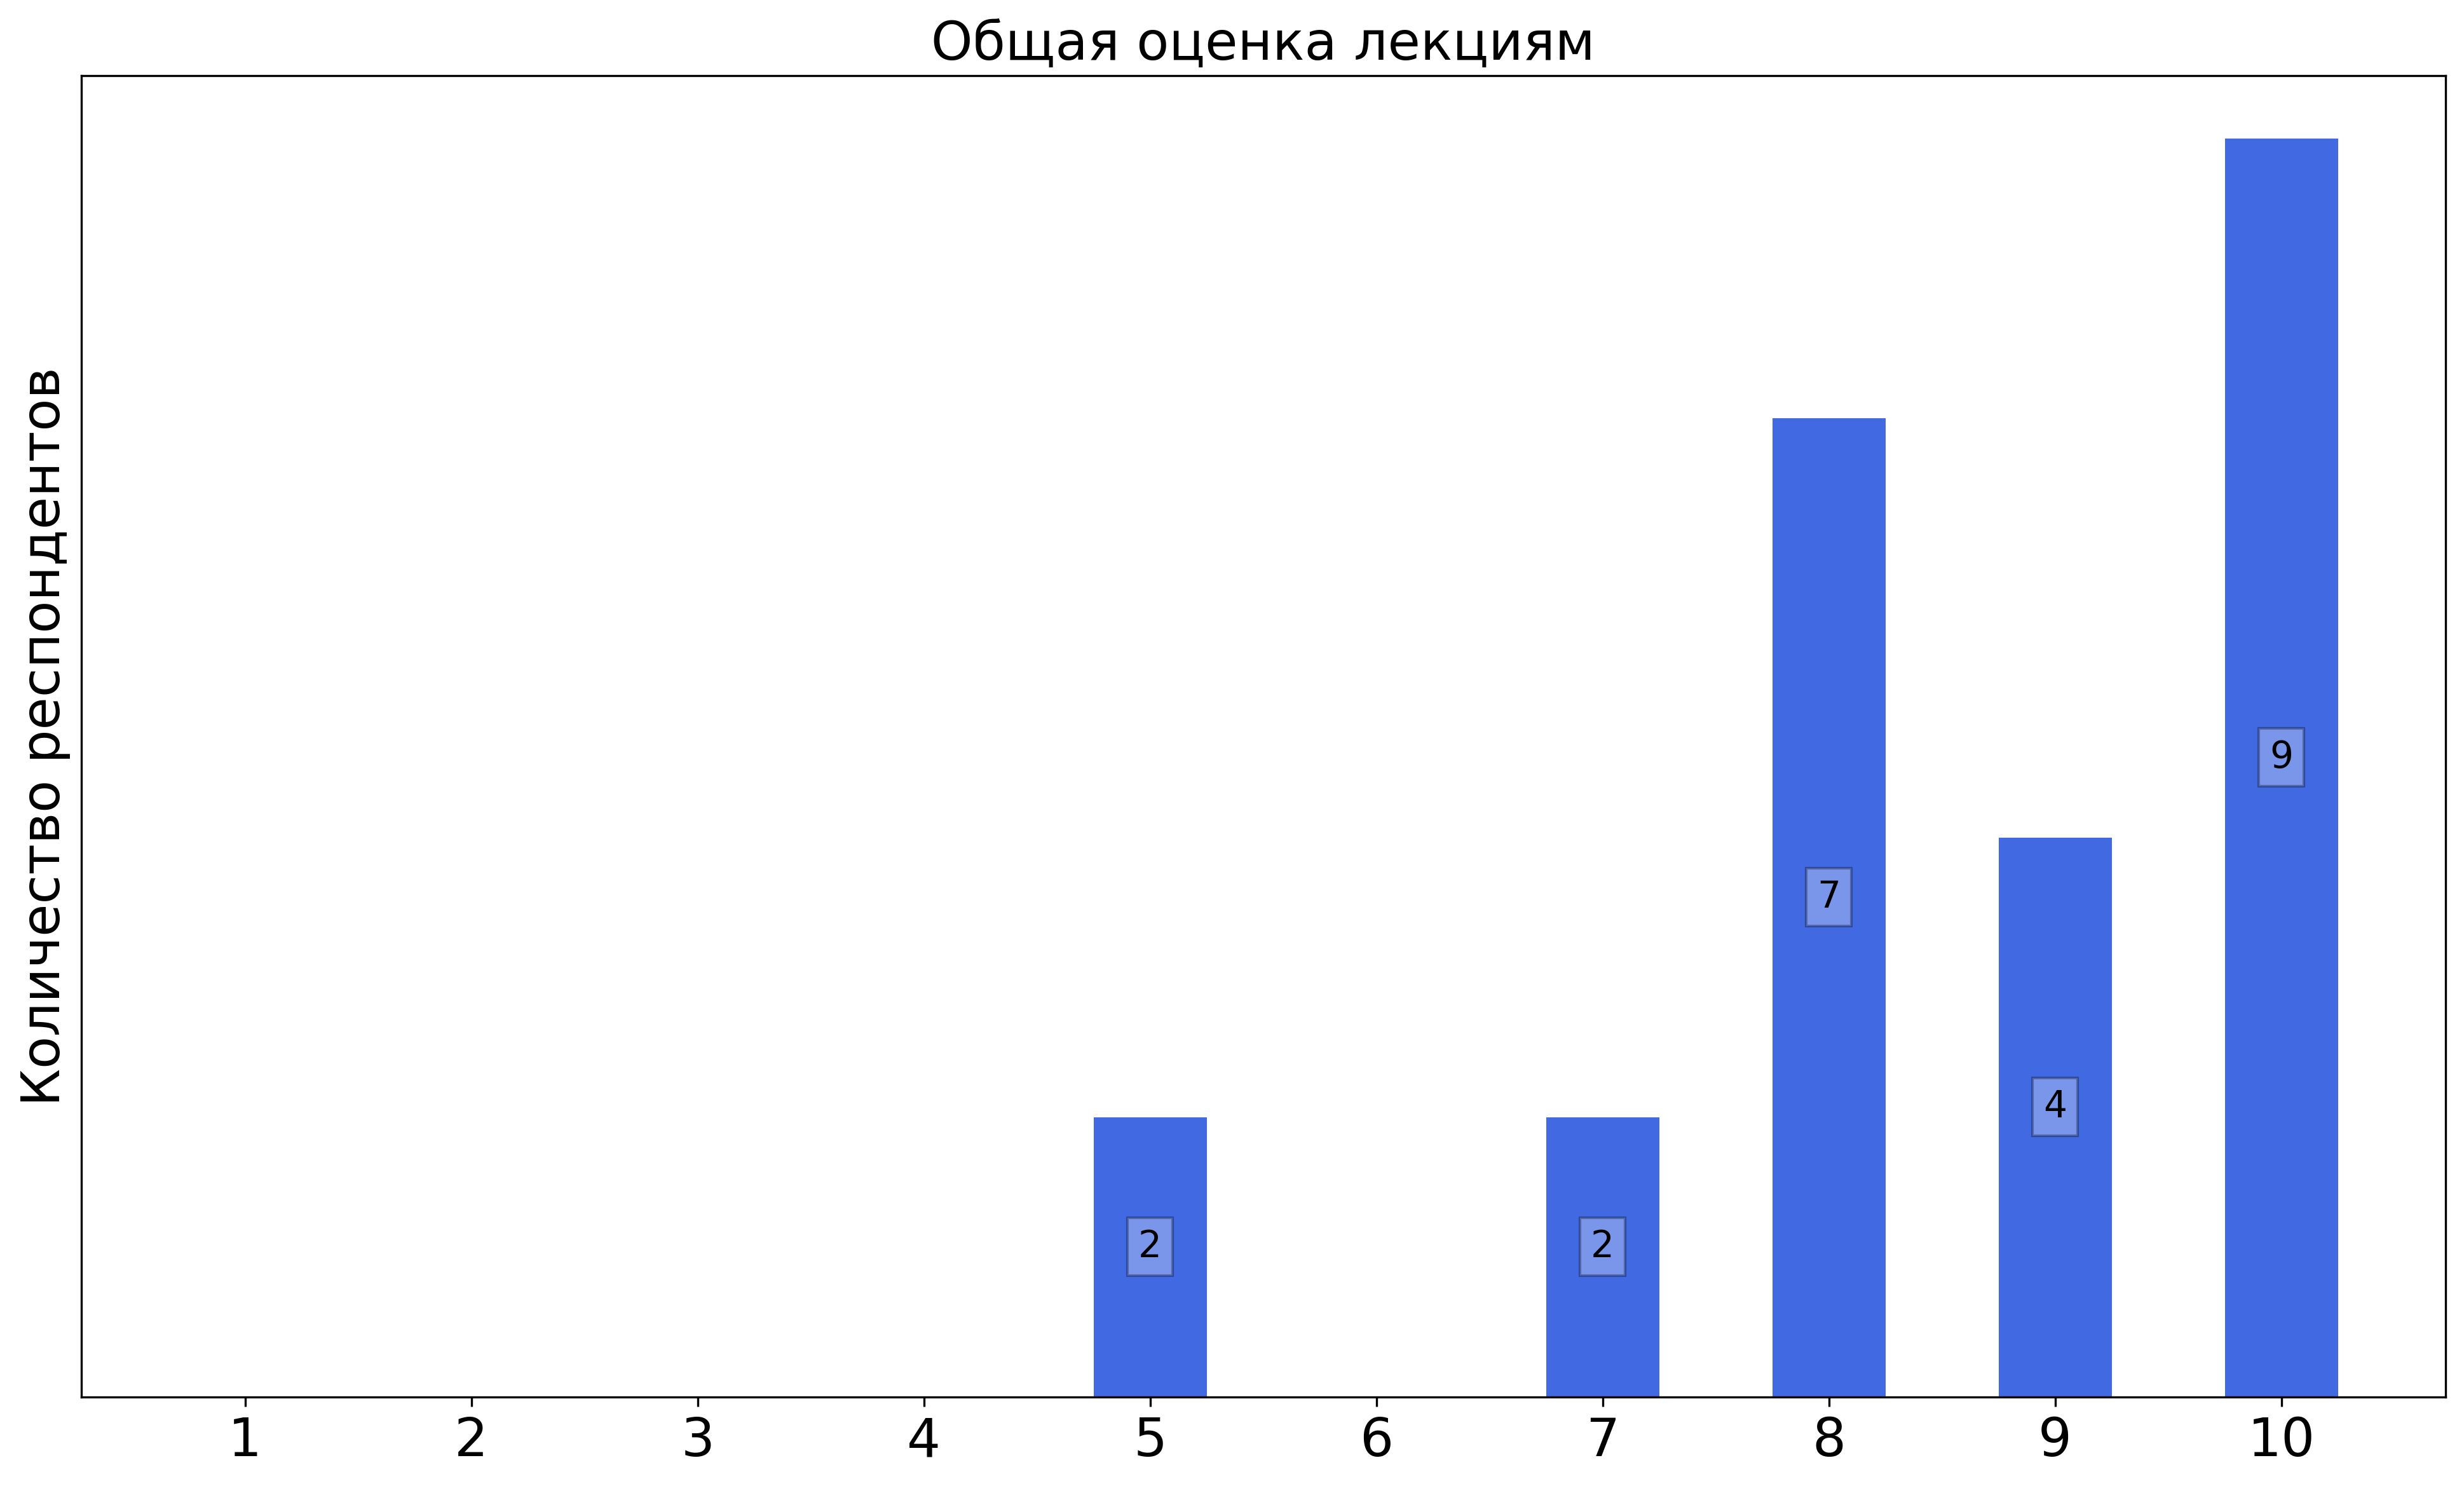
\includegraphics[width=\textwidth]{images/2 course/Аналитическая механика/lecturer-marks-Фомичев А.В.-3.png}
			\end{subfigure}
			\caption{Оценки респондентов о качестве преподавания лекций по курсу <<Аналитическая механика>>}
		\end{figure}

		\textbf{Комментарии студентов о лекциях\protect\footnote{сохранены оригинальные орфография и пунктуация}}
            \begin{commentbox} 
                тяжеловато угнаться за записями и осознать их, после прочтения книг все встает на места 
            \end{commentbox} 
        
            \begin{commentbox} 
                Лектор иногда быстро рассказывает какую то теорему или формулу, не заостряя внимания, а потом постоянно туда ссылается 
            \end{commentbox} 
        
            \begin{commentbox} 
                Слишком много материала... 
            \end{commentbox} 
        
    
    \subsubsection{Отзыв студентов о семинарах. Семинарист: Амелькин Н.И.}
		\begin{figure}[H]
			\centering
			\begin{subfigure}[b]{0.45\textwidth}
				\centering
				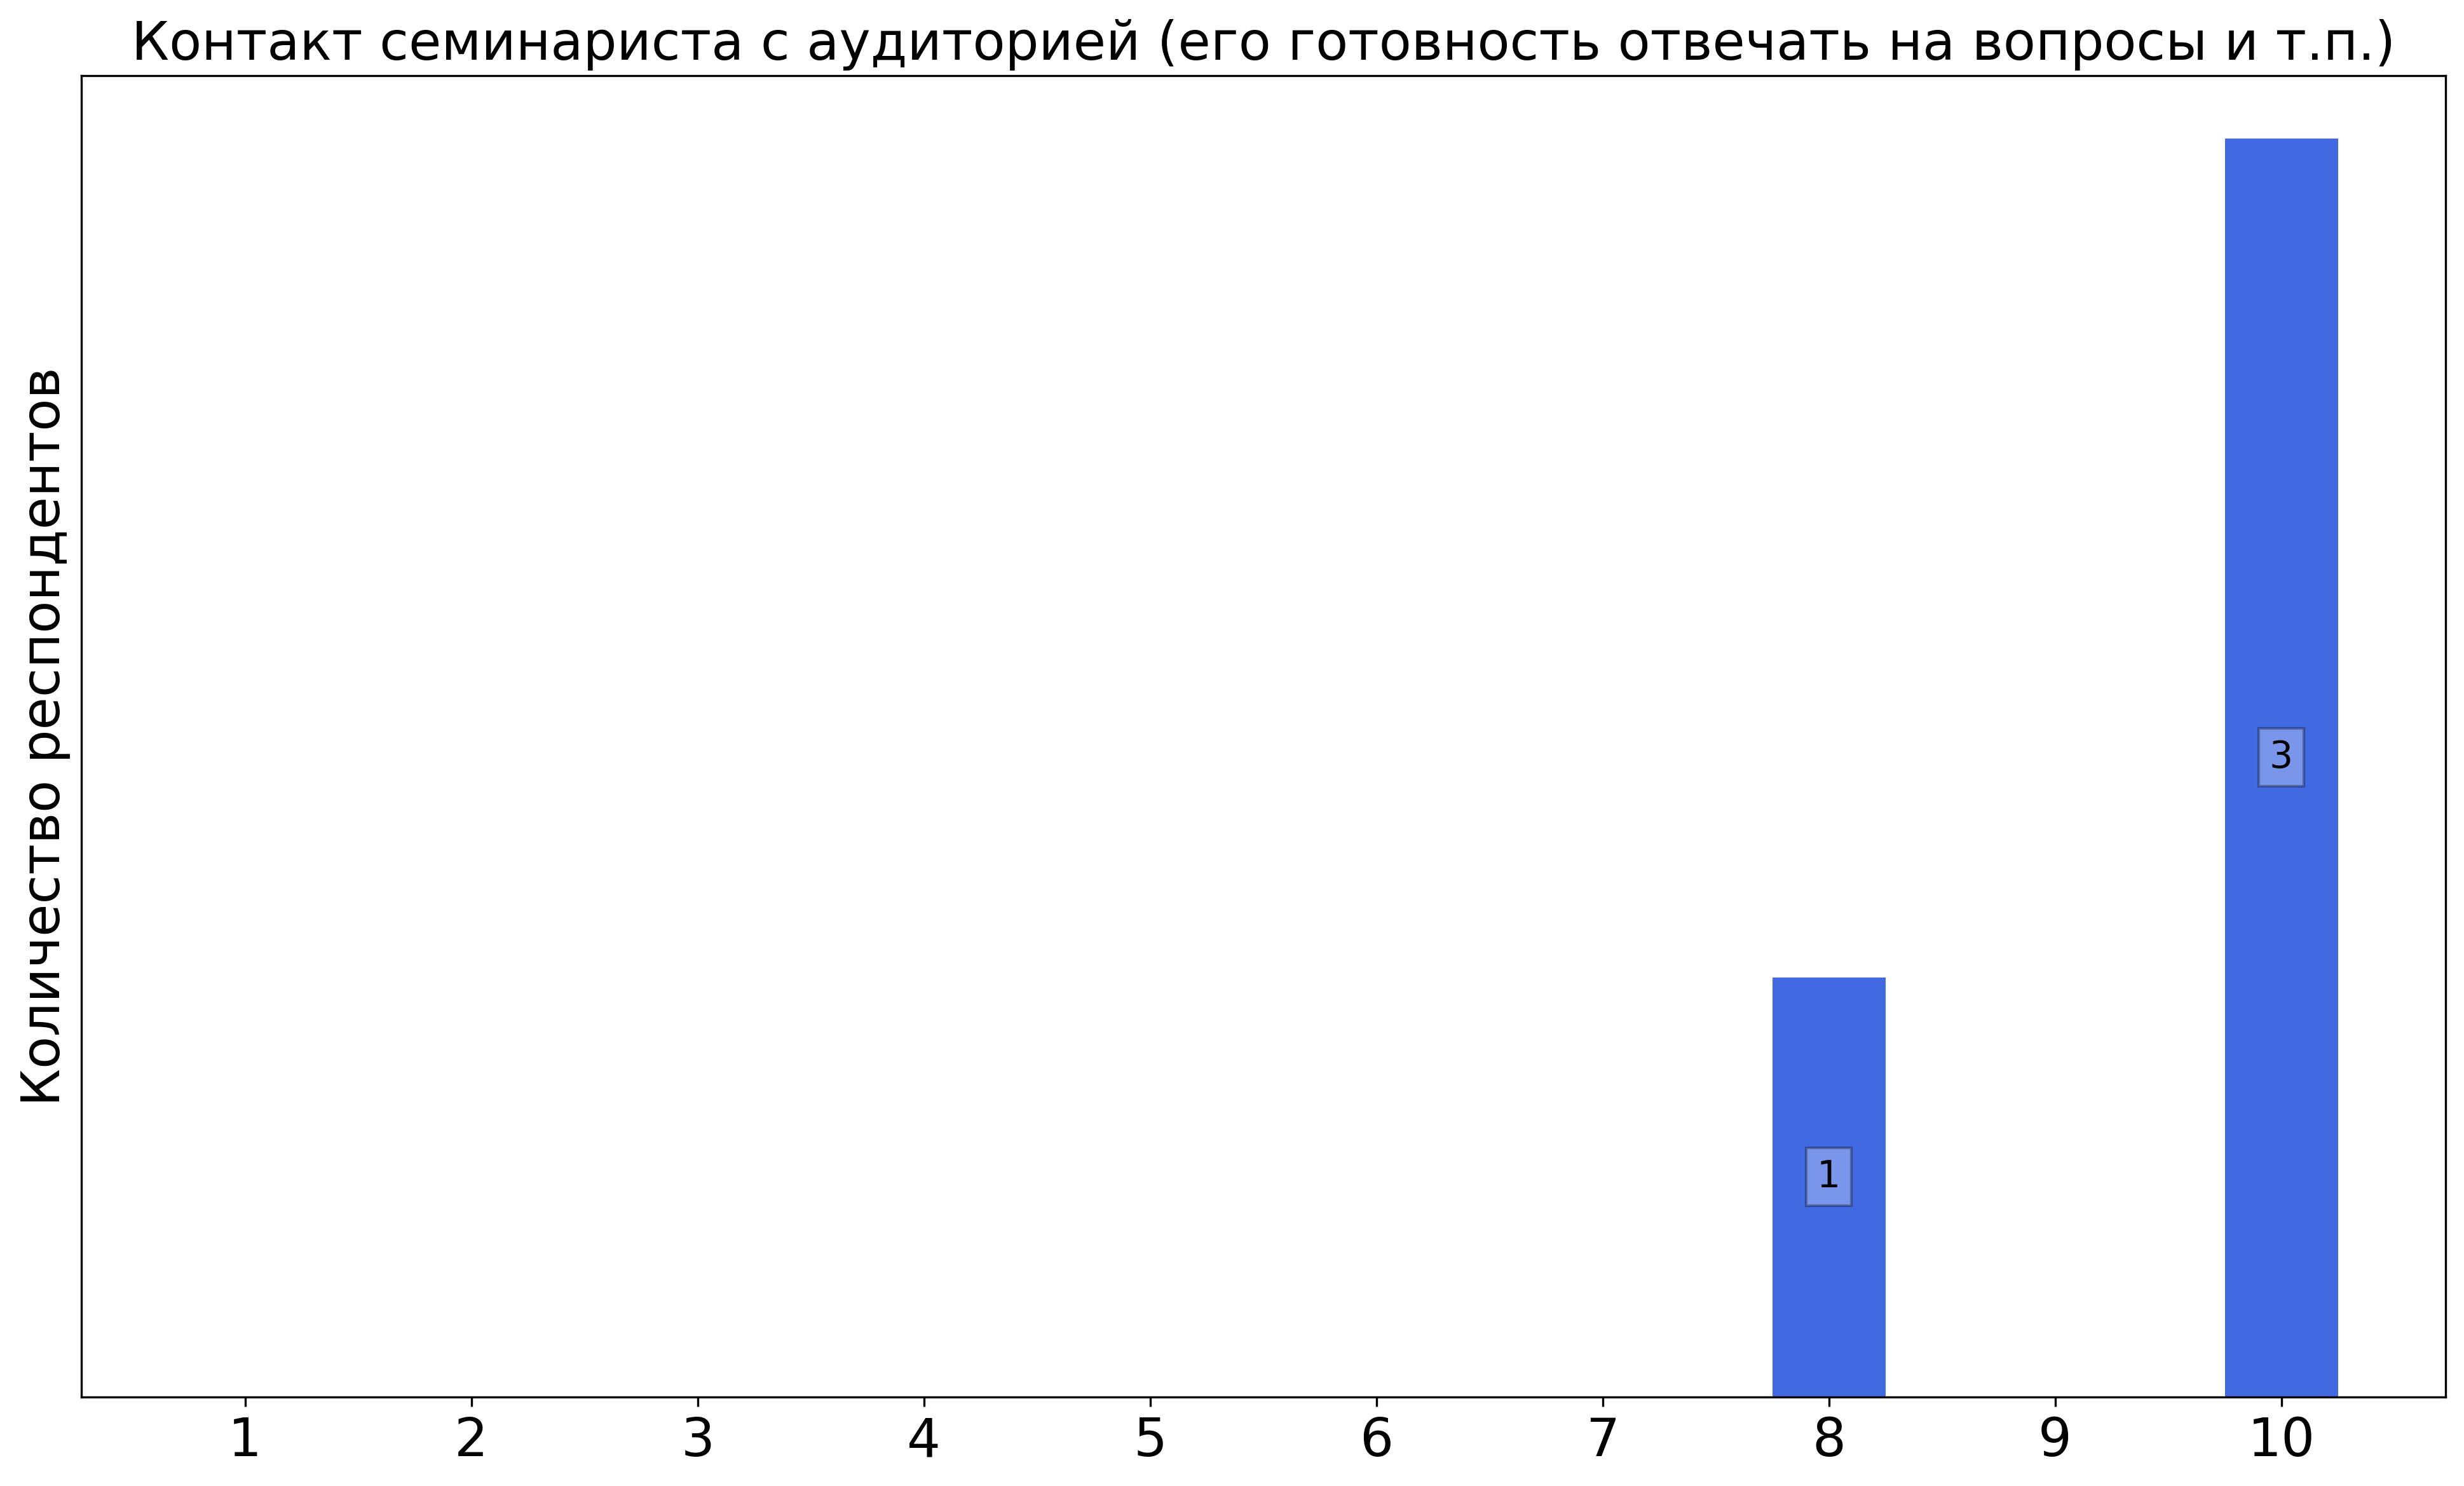
\includegraphics[width=\textwidth]{images/2 course/Аналитическая механика/seminarists-marks-Амелькин Н.И.-0.png}
			\end{subfigure}
			\begin{subfigure}[b]{0.45\textwidth}
				\centering
				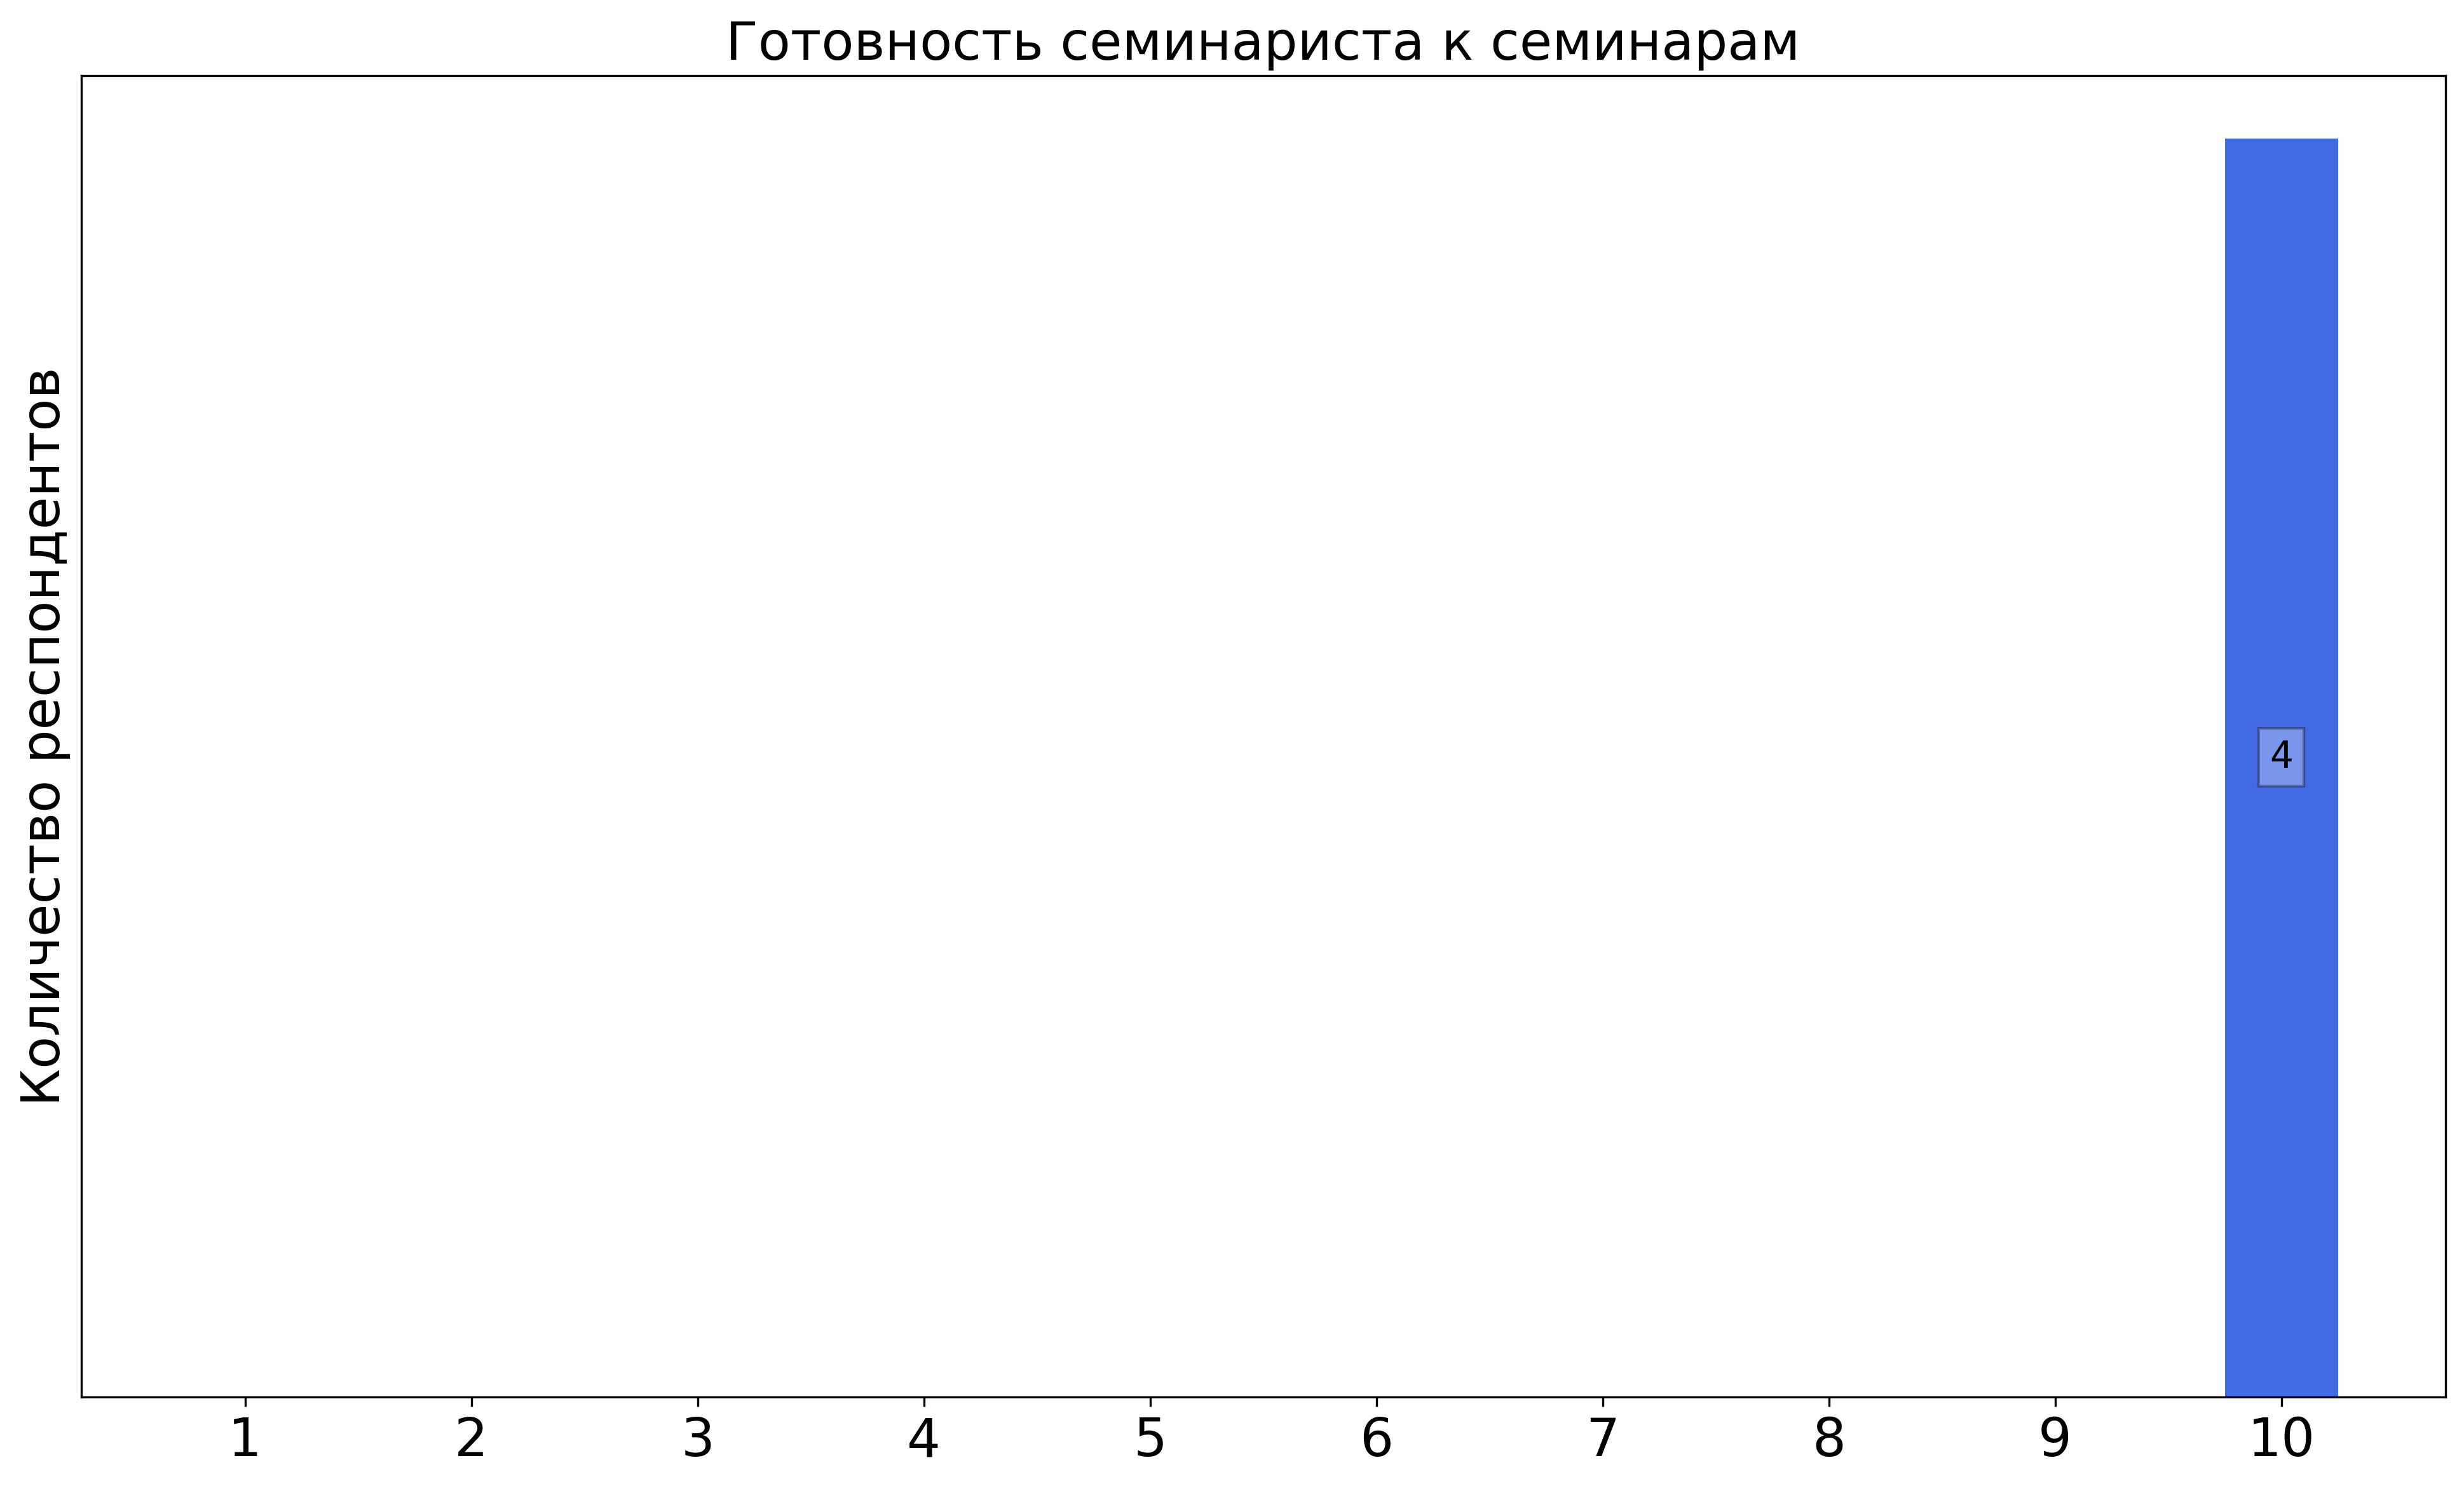
\includegraphics[width=\textwidth]{images/2 course/Аналитическая механика/seminarists-marks-Амелькин Н.И.-1.png}
			\end{subfigure}
			\begin{subfigure}[b]{0.45\textwidth}
				\centering
				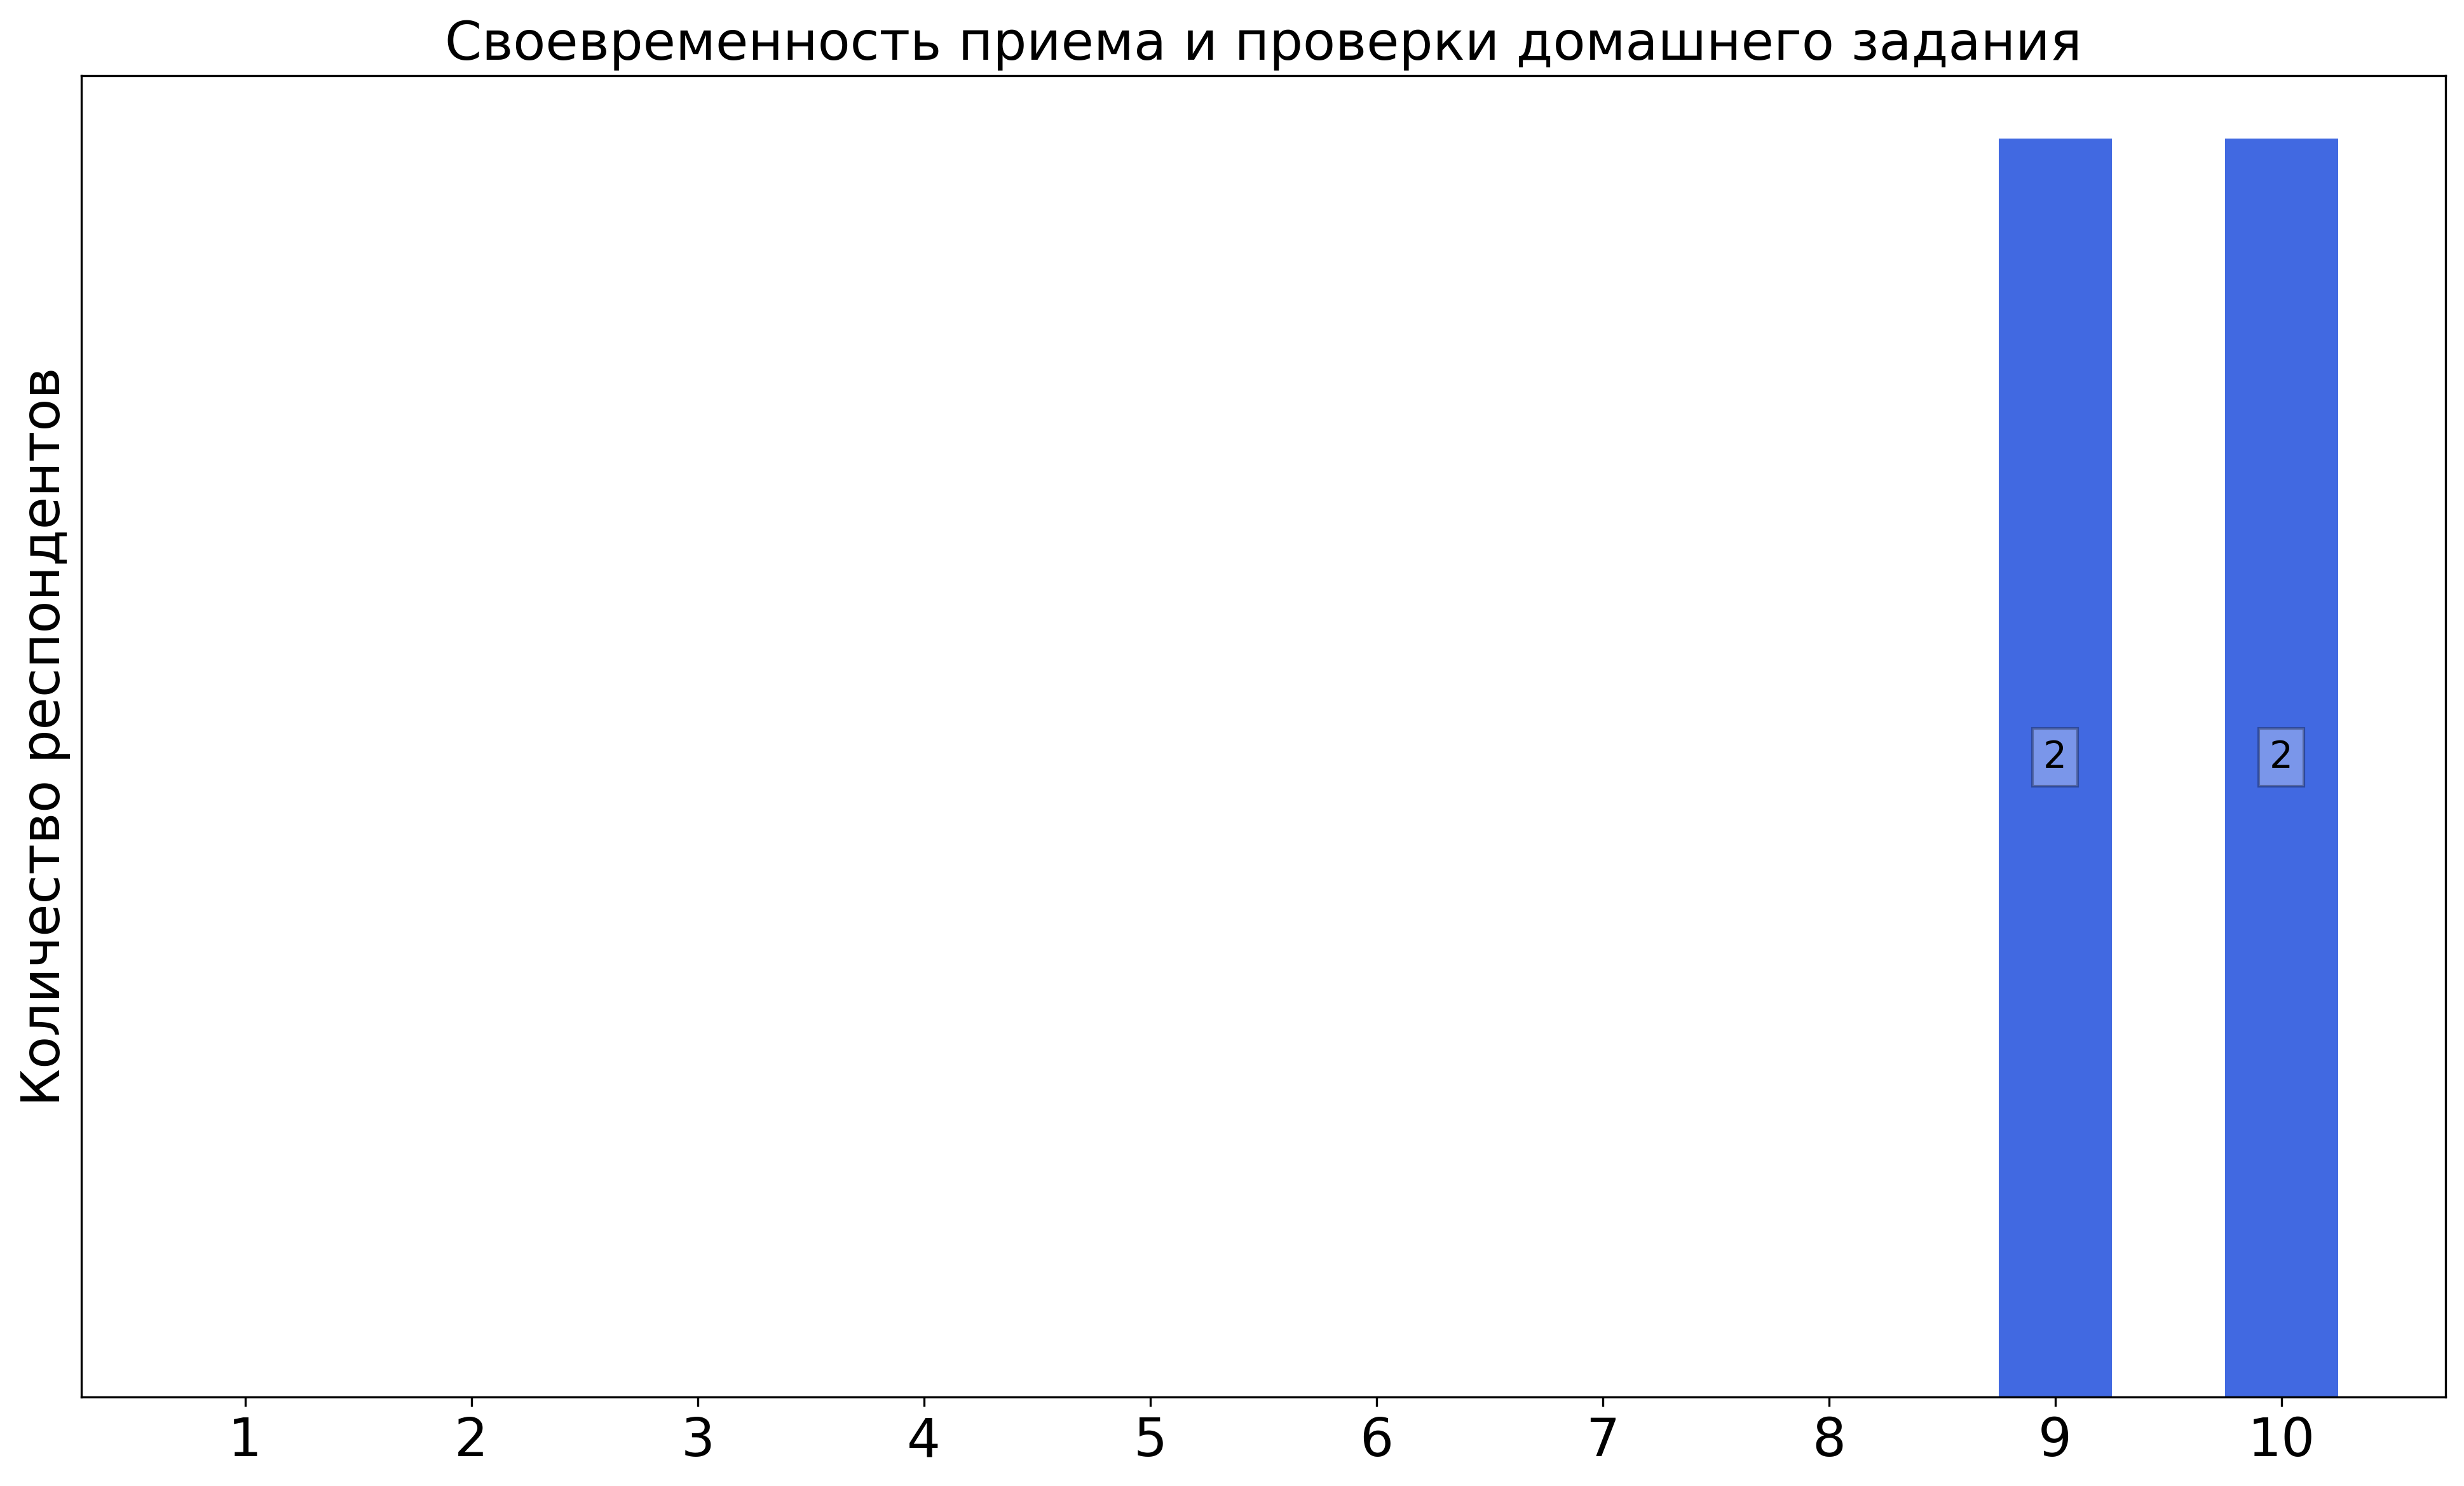
\includegraphics[width=\textwidth]{images/2 course/Аналитическая механика/seminarists-marks-Амелькин Н.И.-2.png}
			\end{subfigure}
			\begin{subfigure}[b]{0.45\textwidth}
				\centering
				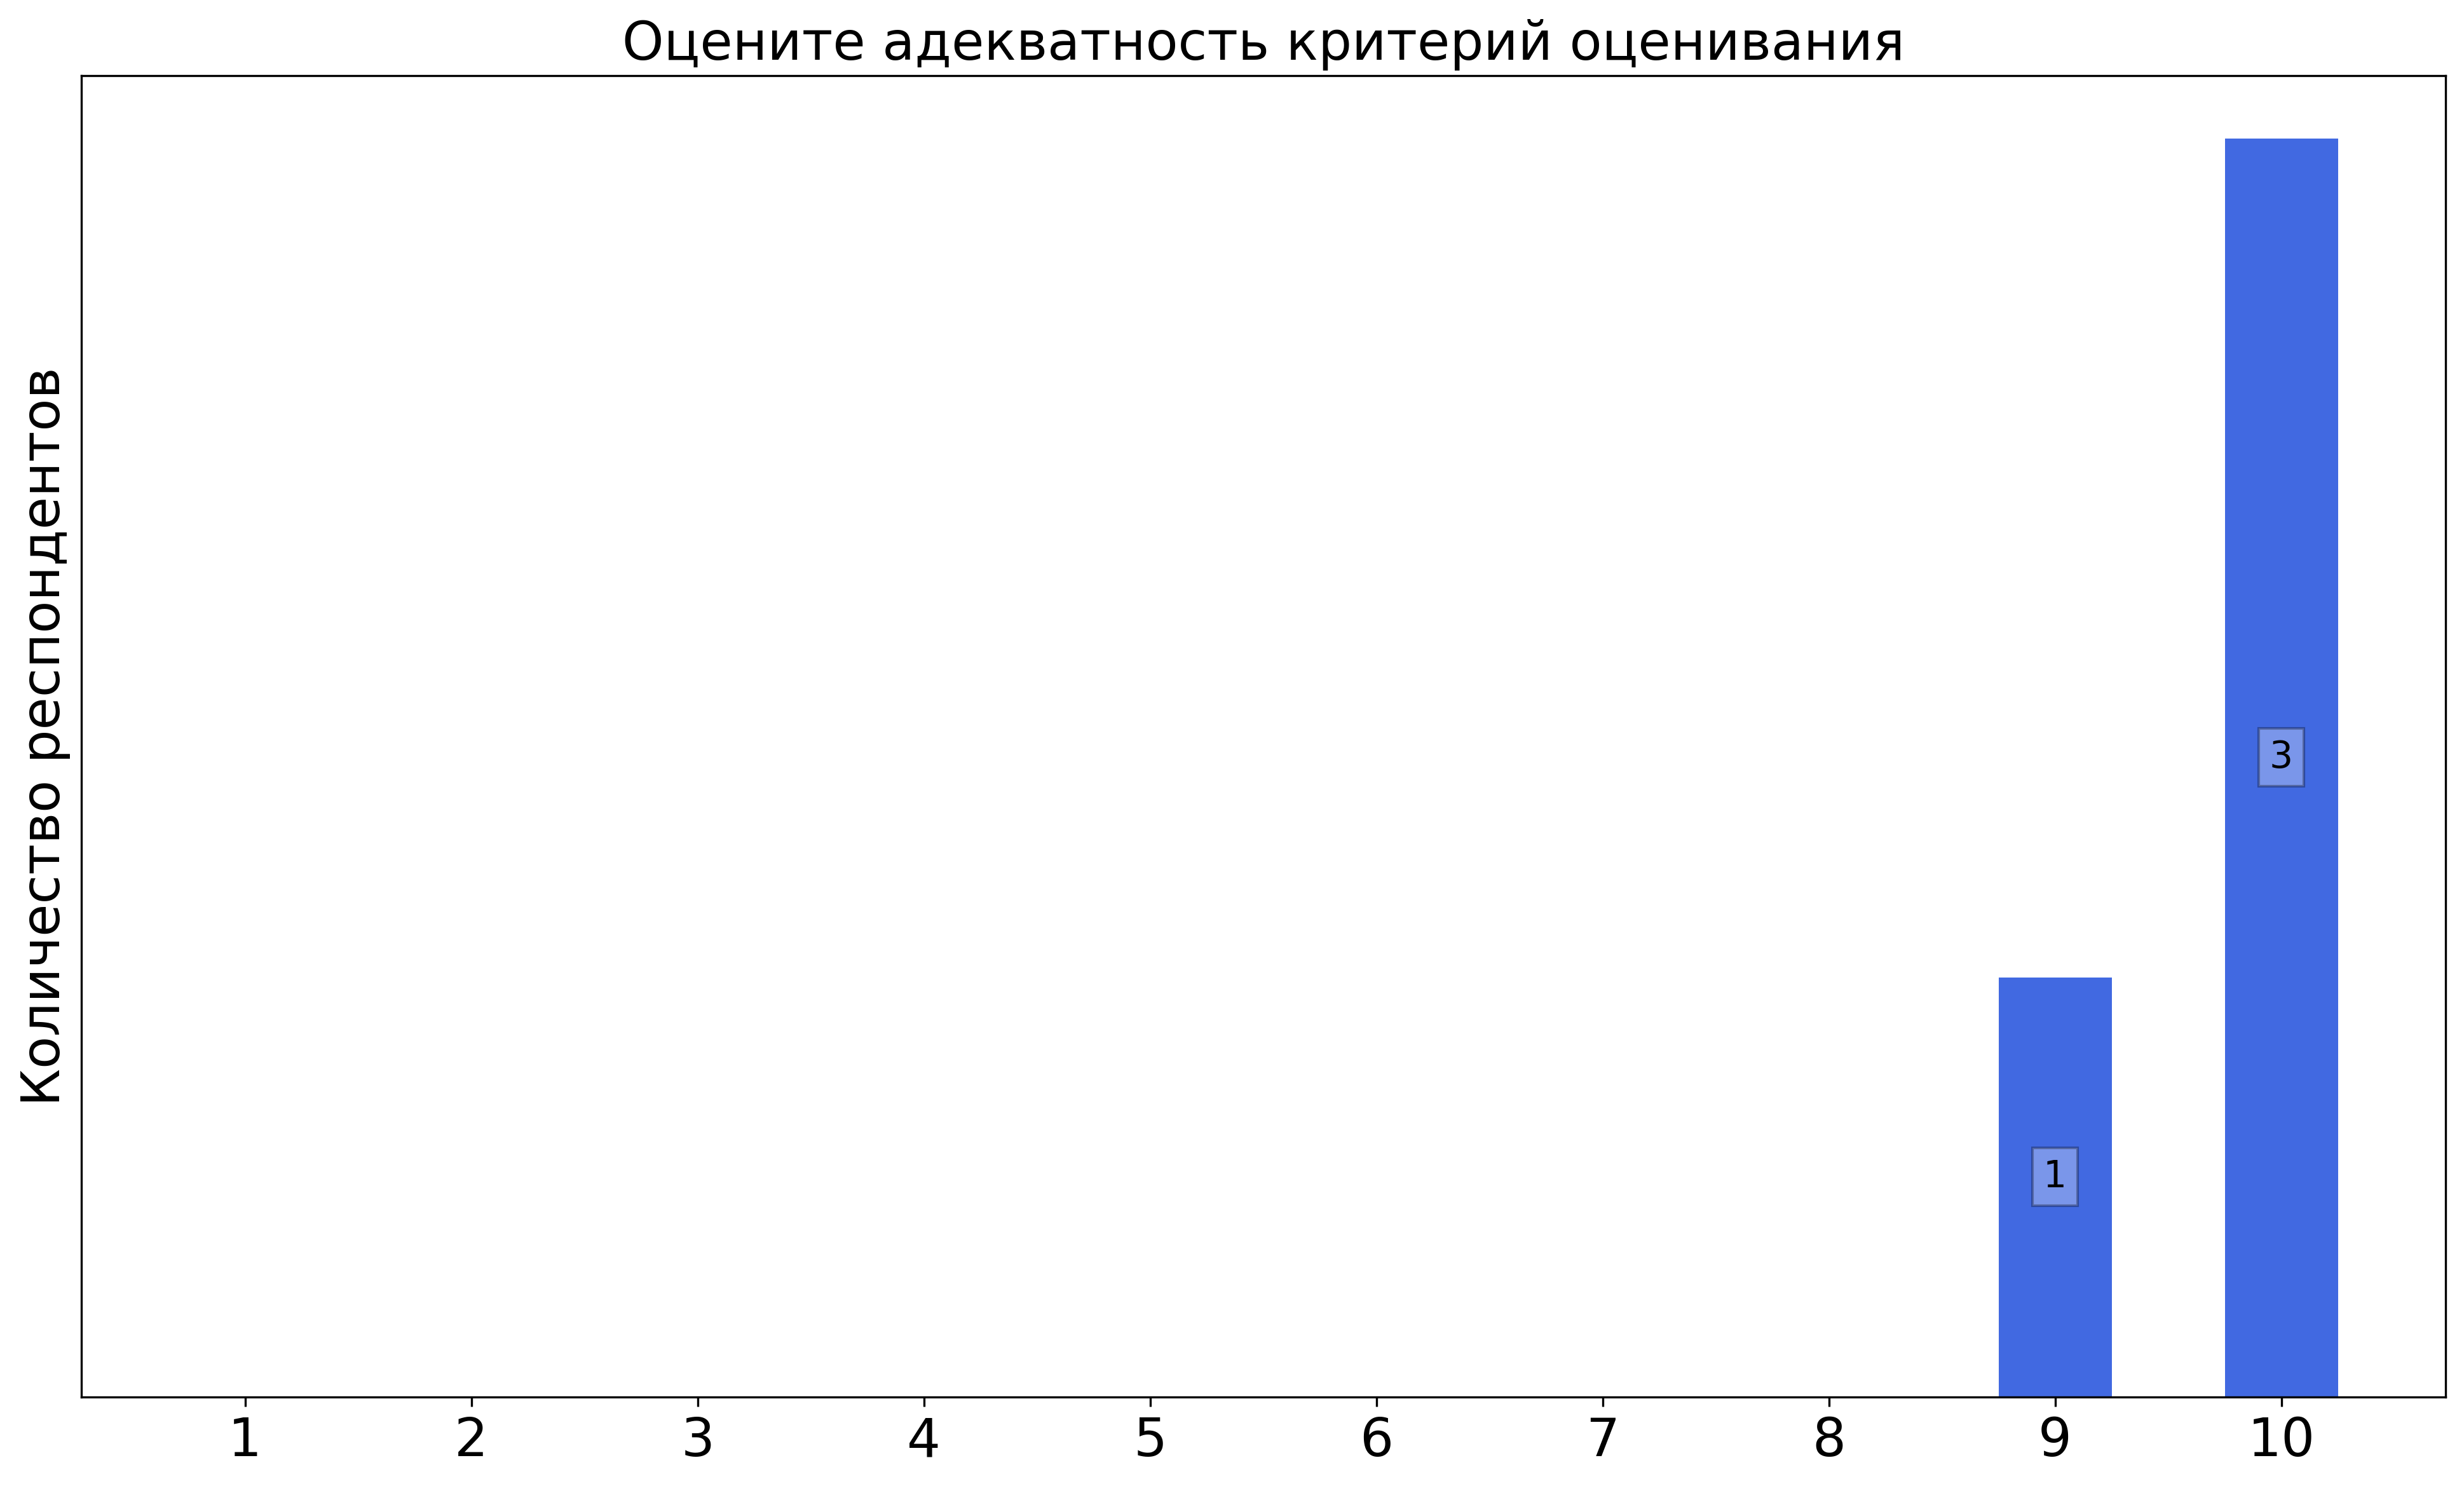
\includegraphics[width=\textwidth]{images/2 course/Аналитическая механика/seminarists-marks-Амелькин Н.И.-3.png}
			\end{subfigure}	
			\caption{Оценки респондентов о качестве преподавания семинаров}
		\end{figure}

		\textbf{Комментарии студентов о семинаристе\protect\footnote{сохранены оригинальные орфография и пунктуация}}
            \begin{commentbox} 
                Было полезно посещать семинары, так как на каждом из них были повторения лекционного материала и были изложены необходимые теоретические выкладки 
            \end{commentbox}

    
    \subsubsection{Отзыв студентов о семинарах. Семинарист: Ахлумади Махди Реза}
        \begin{figure}[H]
            \centering
            \begin{subfigure}[b]{0.45\textwidth}
                \centering
                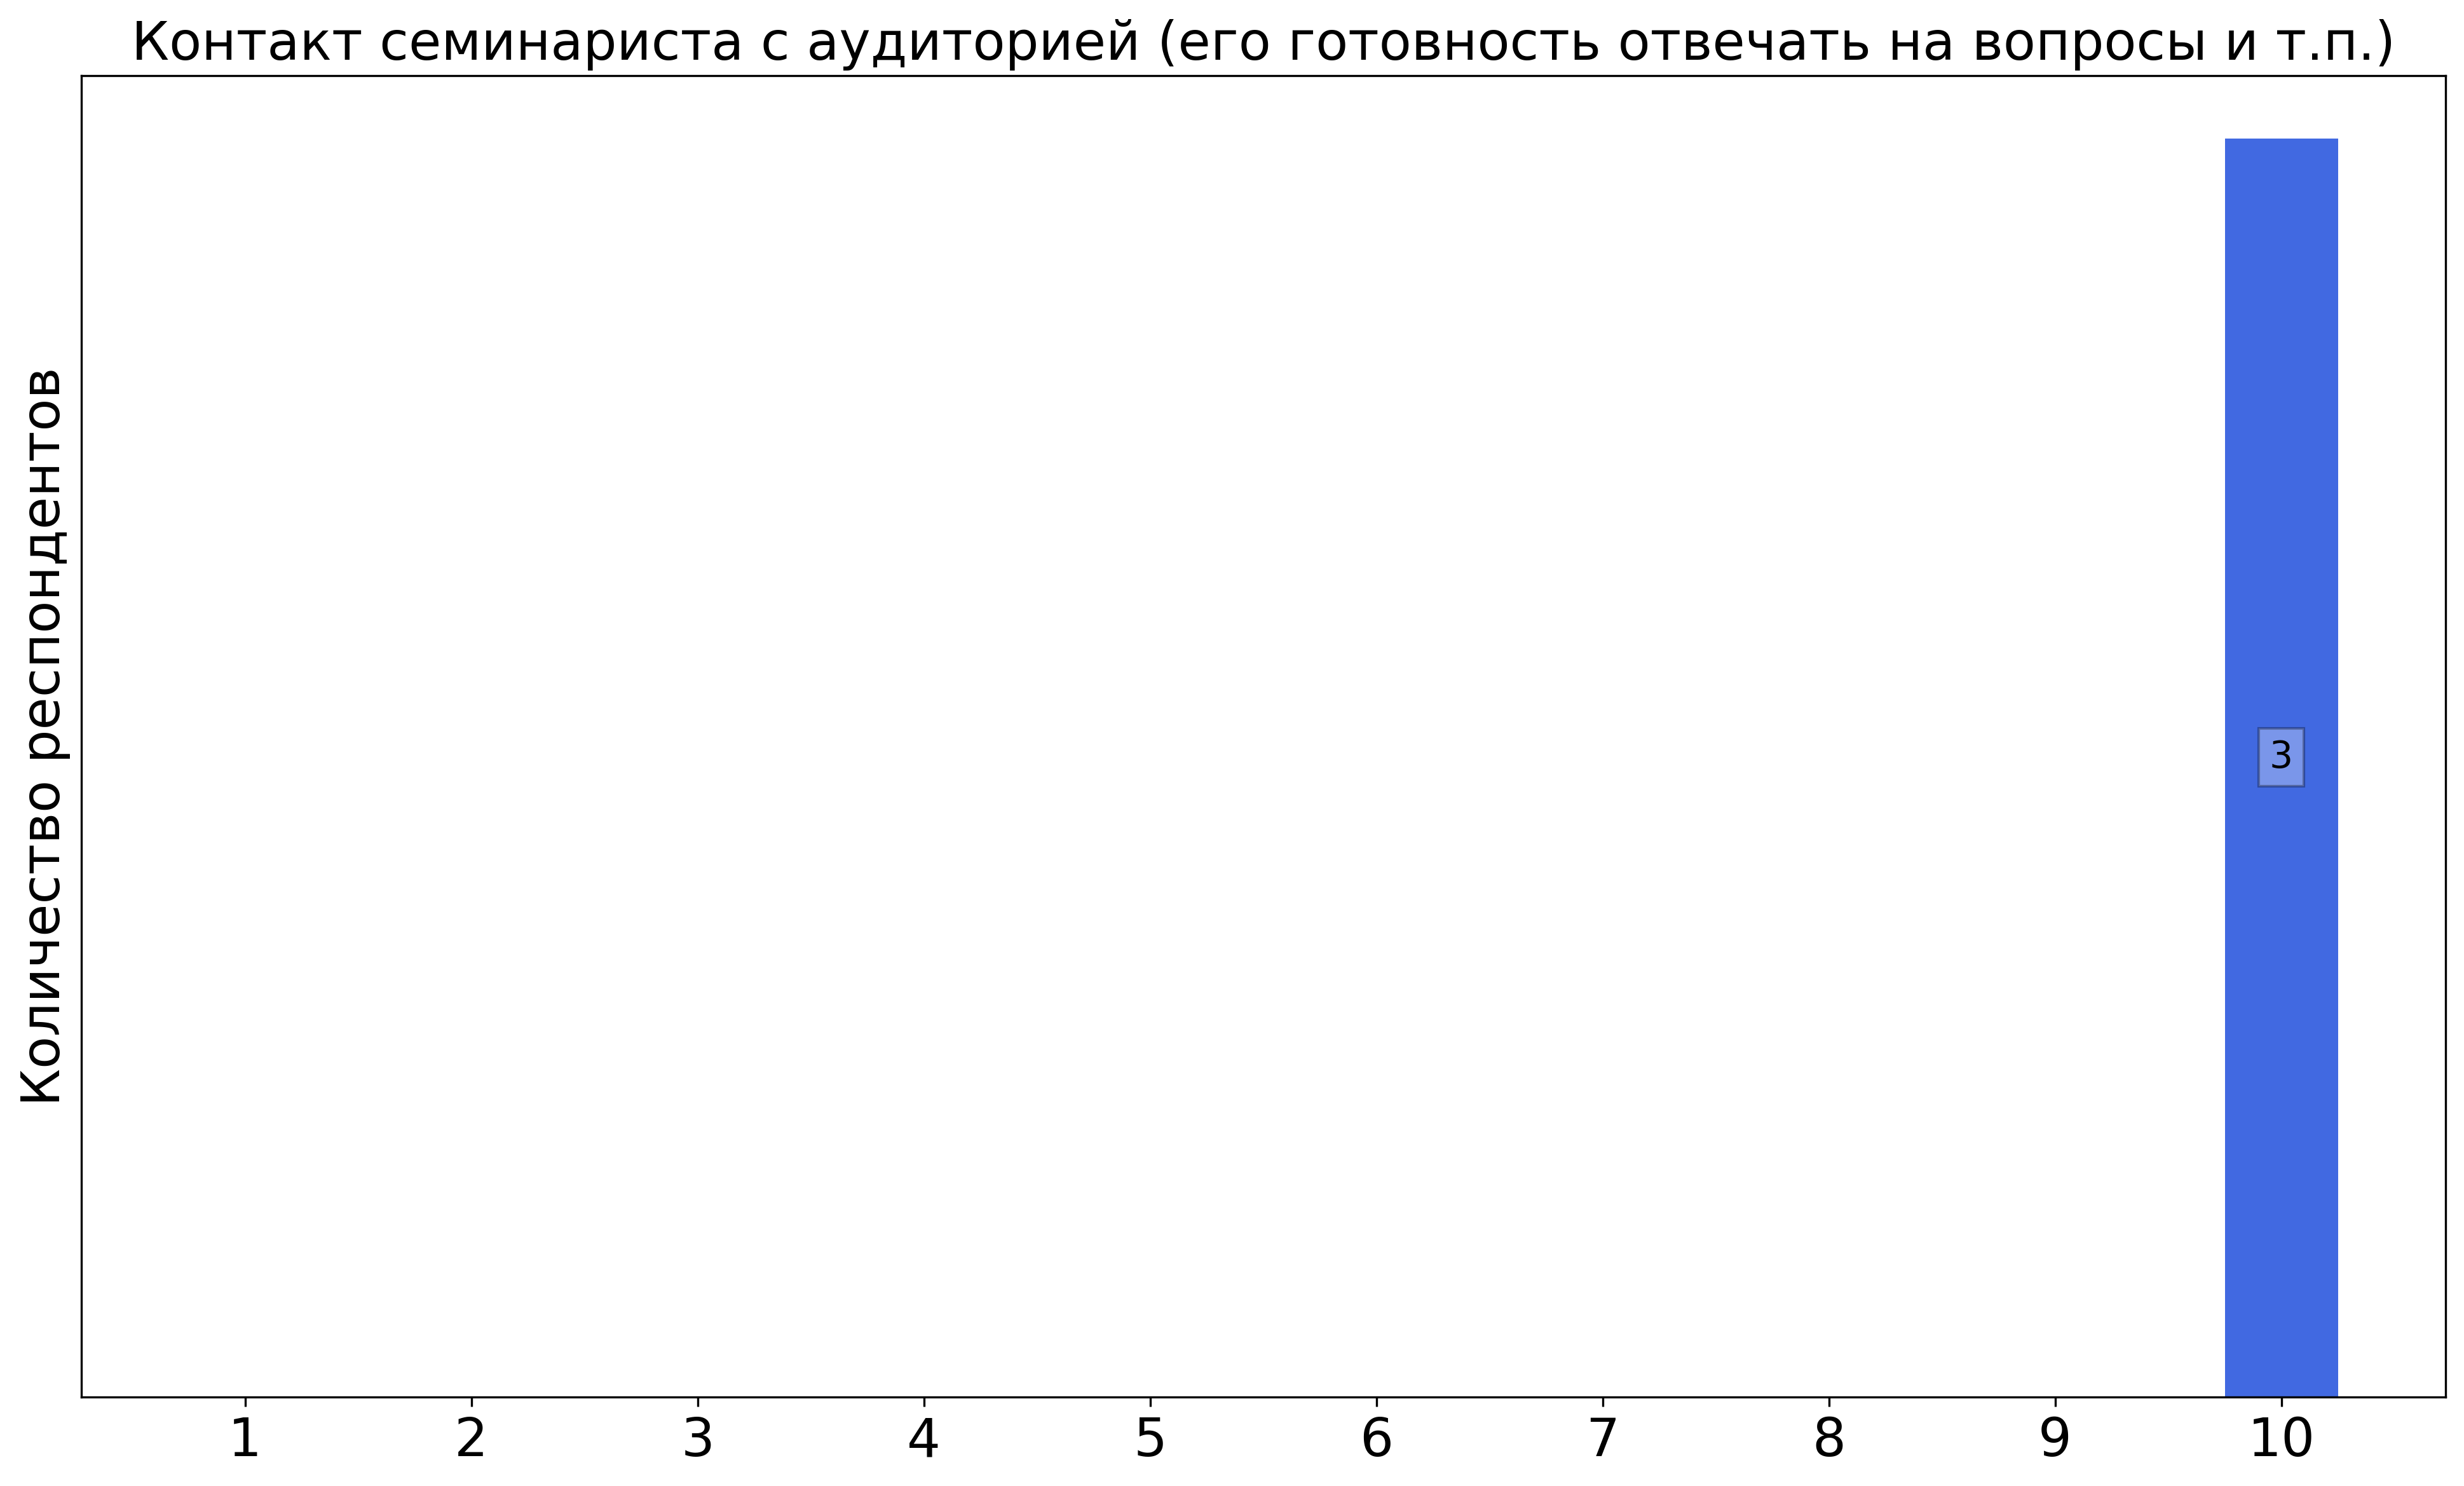
\includegraphics[width=\textwidth]{images/2 course/Аналитическая механика/seminarists-marks-Ахлумади Махди Реза-0.png}
            \end{subfigure}
            \begin{subfigure}[b]{0.45\textwidth}
                \centering
                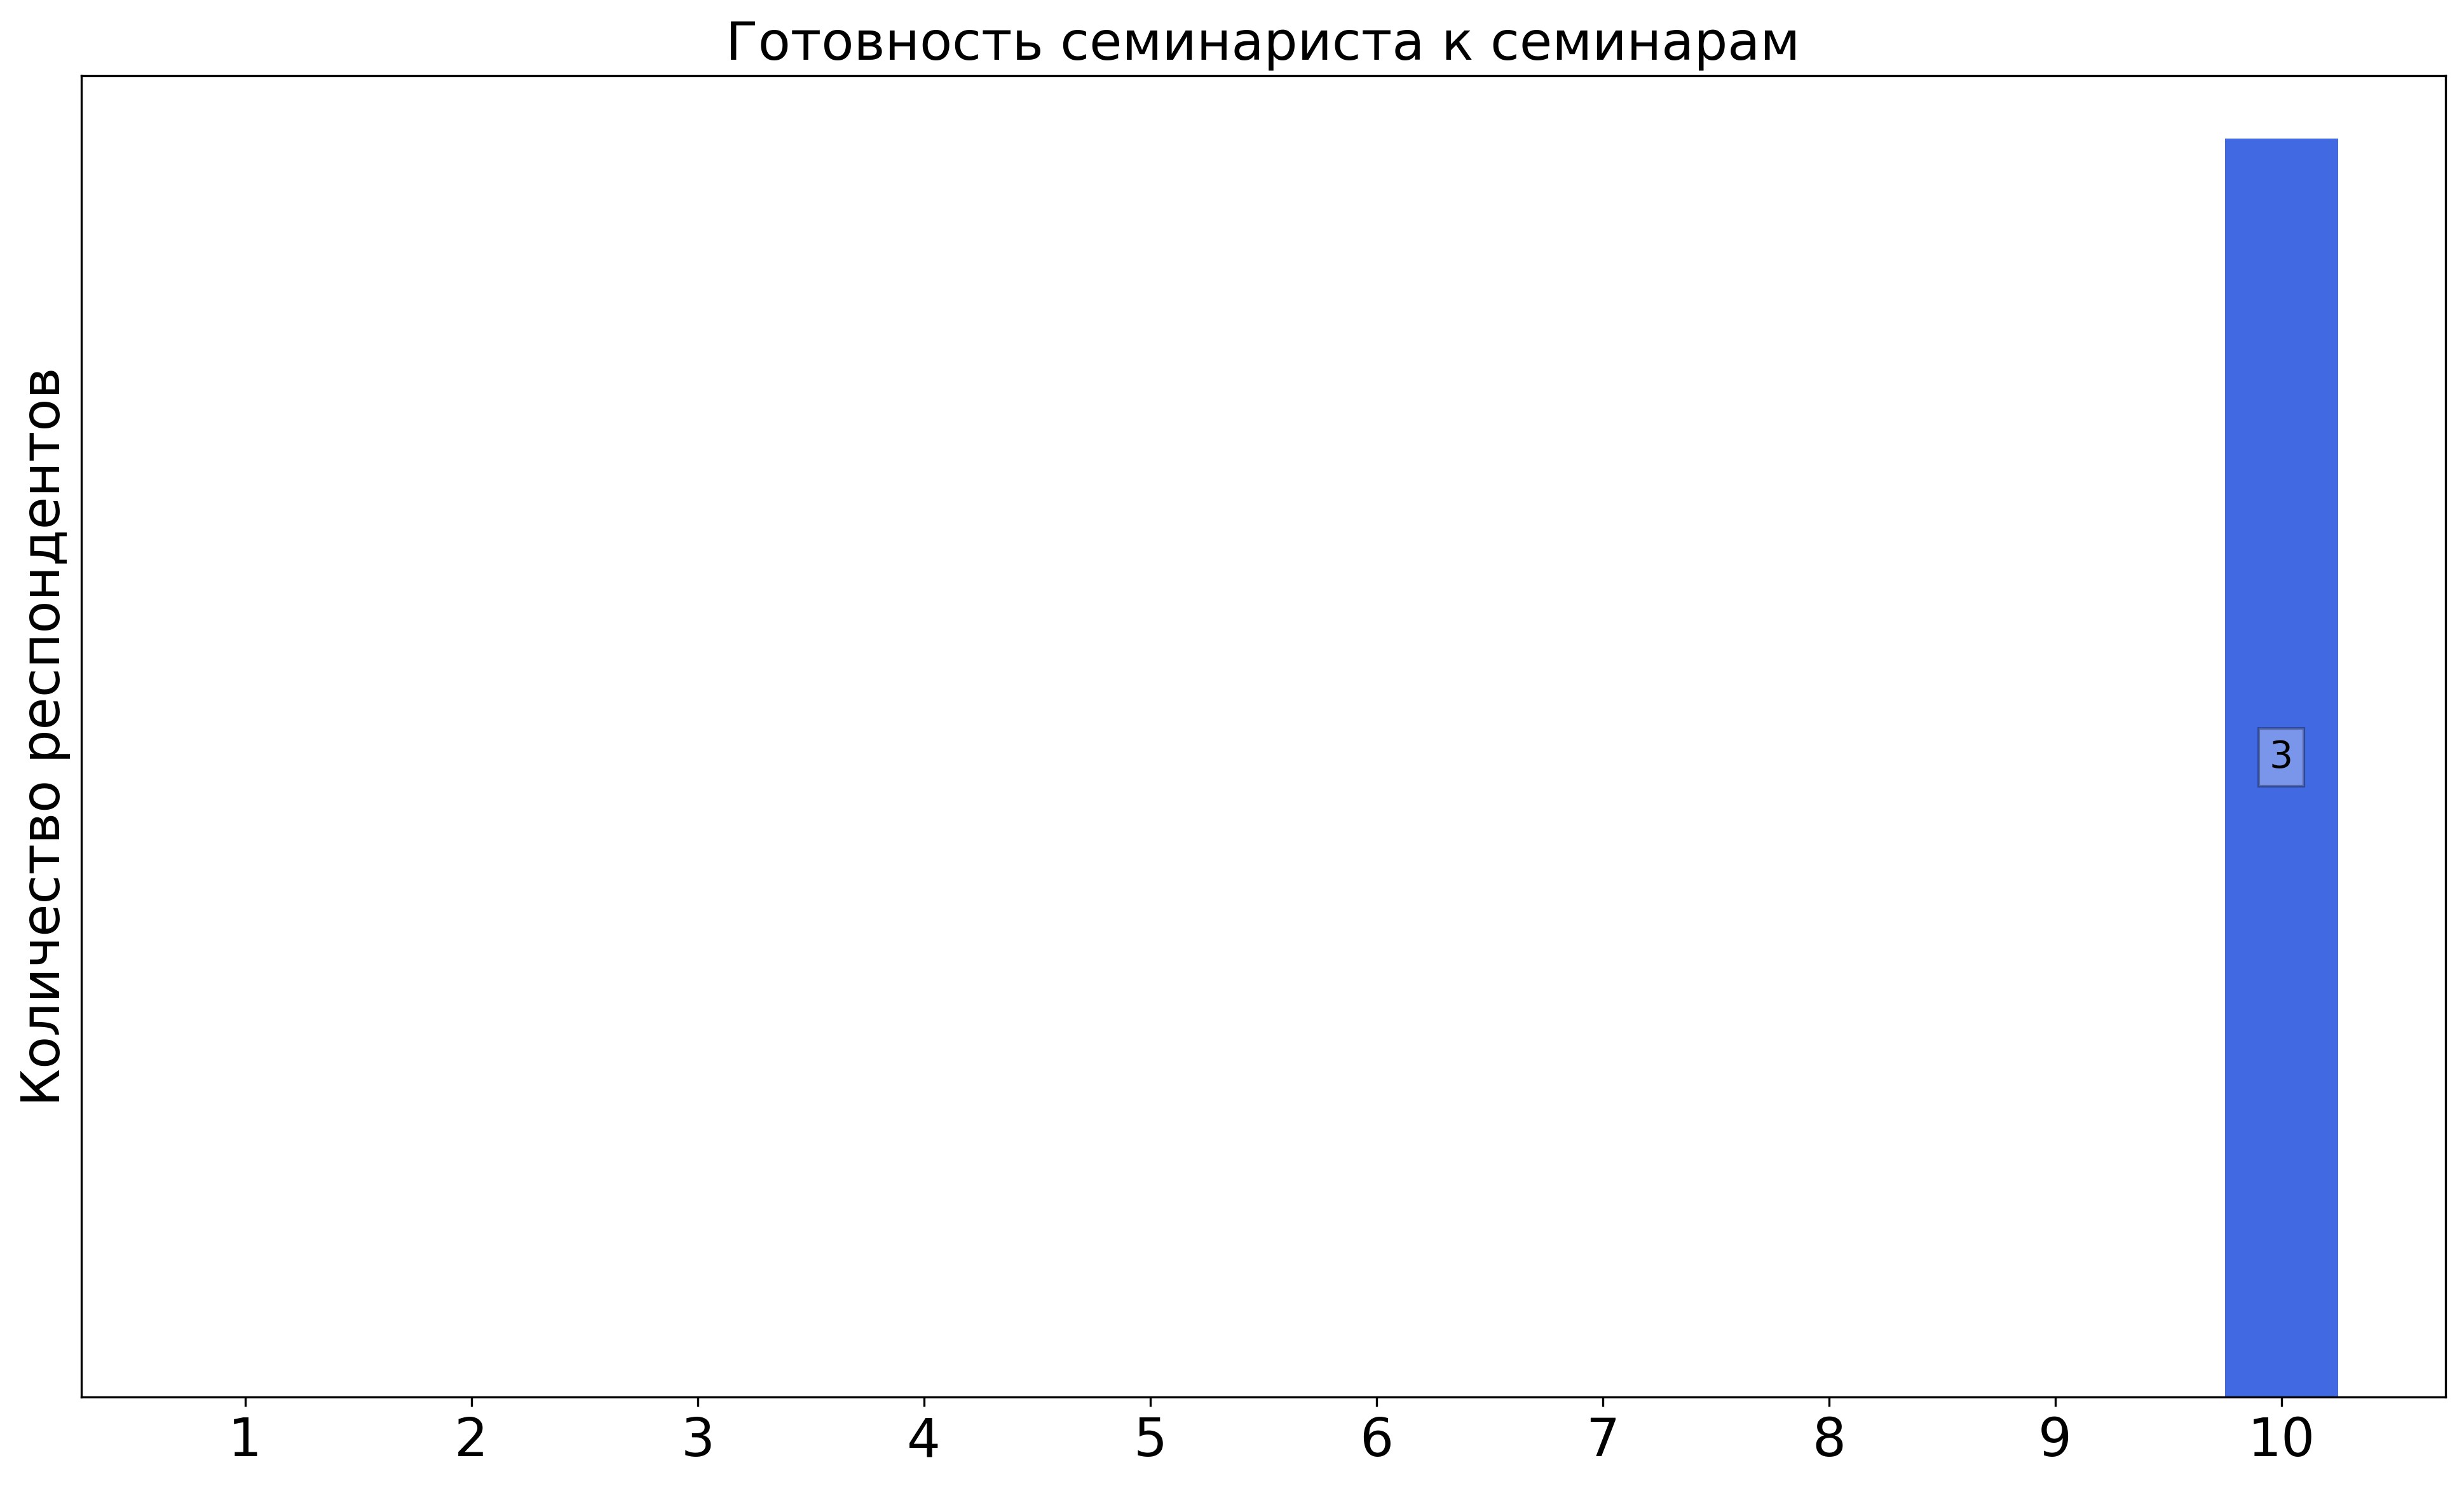
\includegraphics[width=\textwidth]{images/2 course/Аналитическая механика/seminarists-marks-Ахлумади Махди Реза-1.png}
            \end{subfigure}
            \begin{subfigure}[b]{0.45\textwidth}
                \centering
                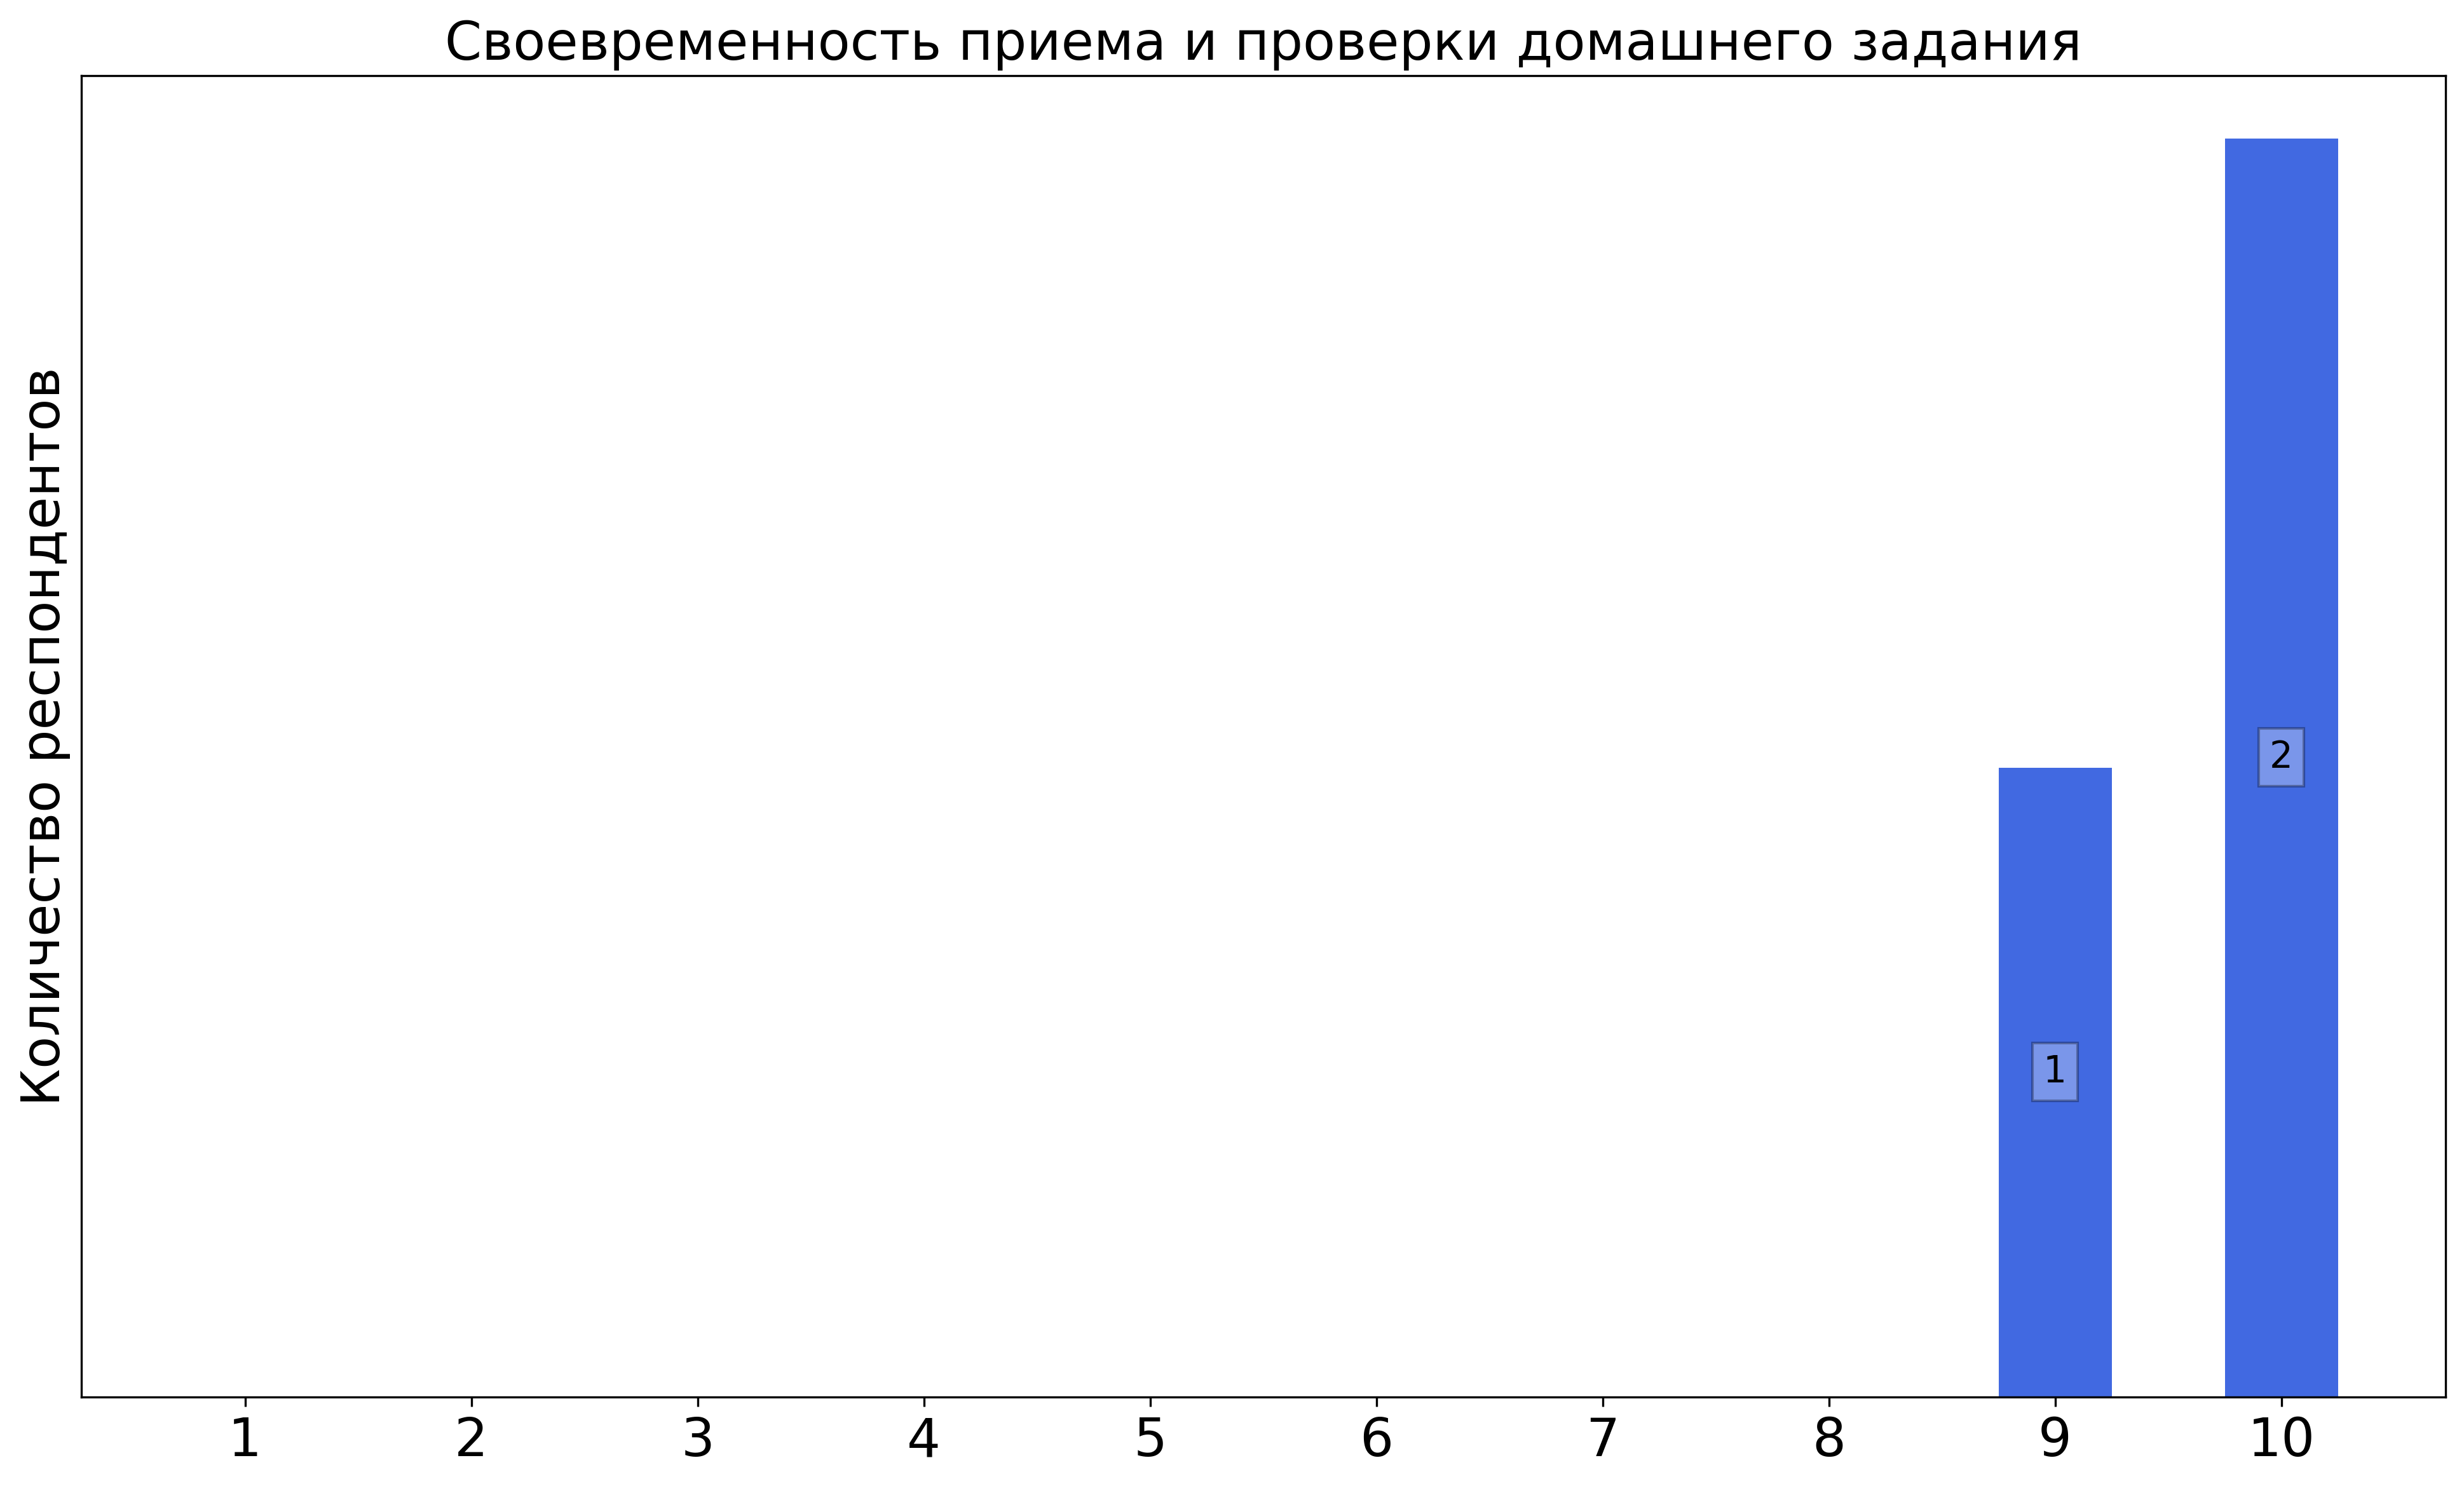
\includegraphics[width=\textwidth]{images/2 course/Аналитическая механика/seminarists-marks-Ахлумади Махди Реза-2.png}
            \end{subfigure}
            \begin{subfigure}[b]{0.45\textwidth}
                \centering
                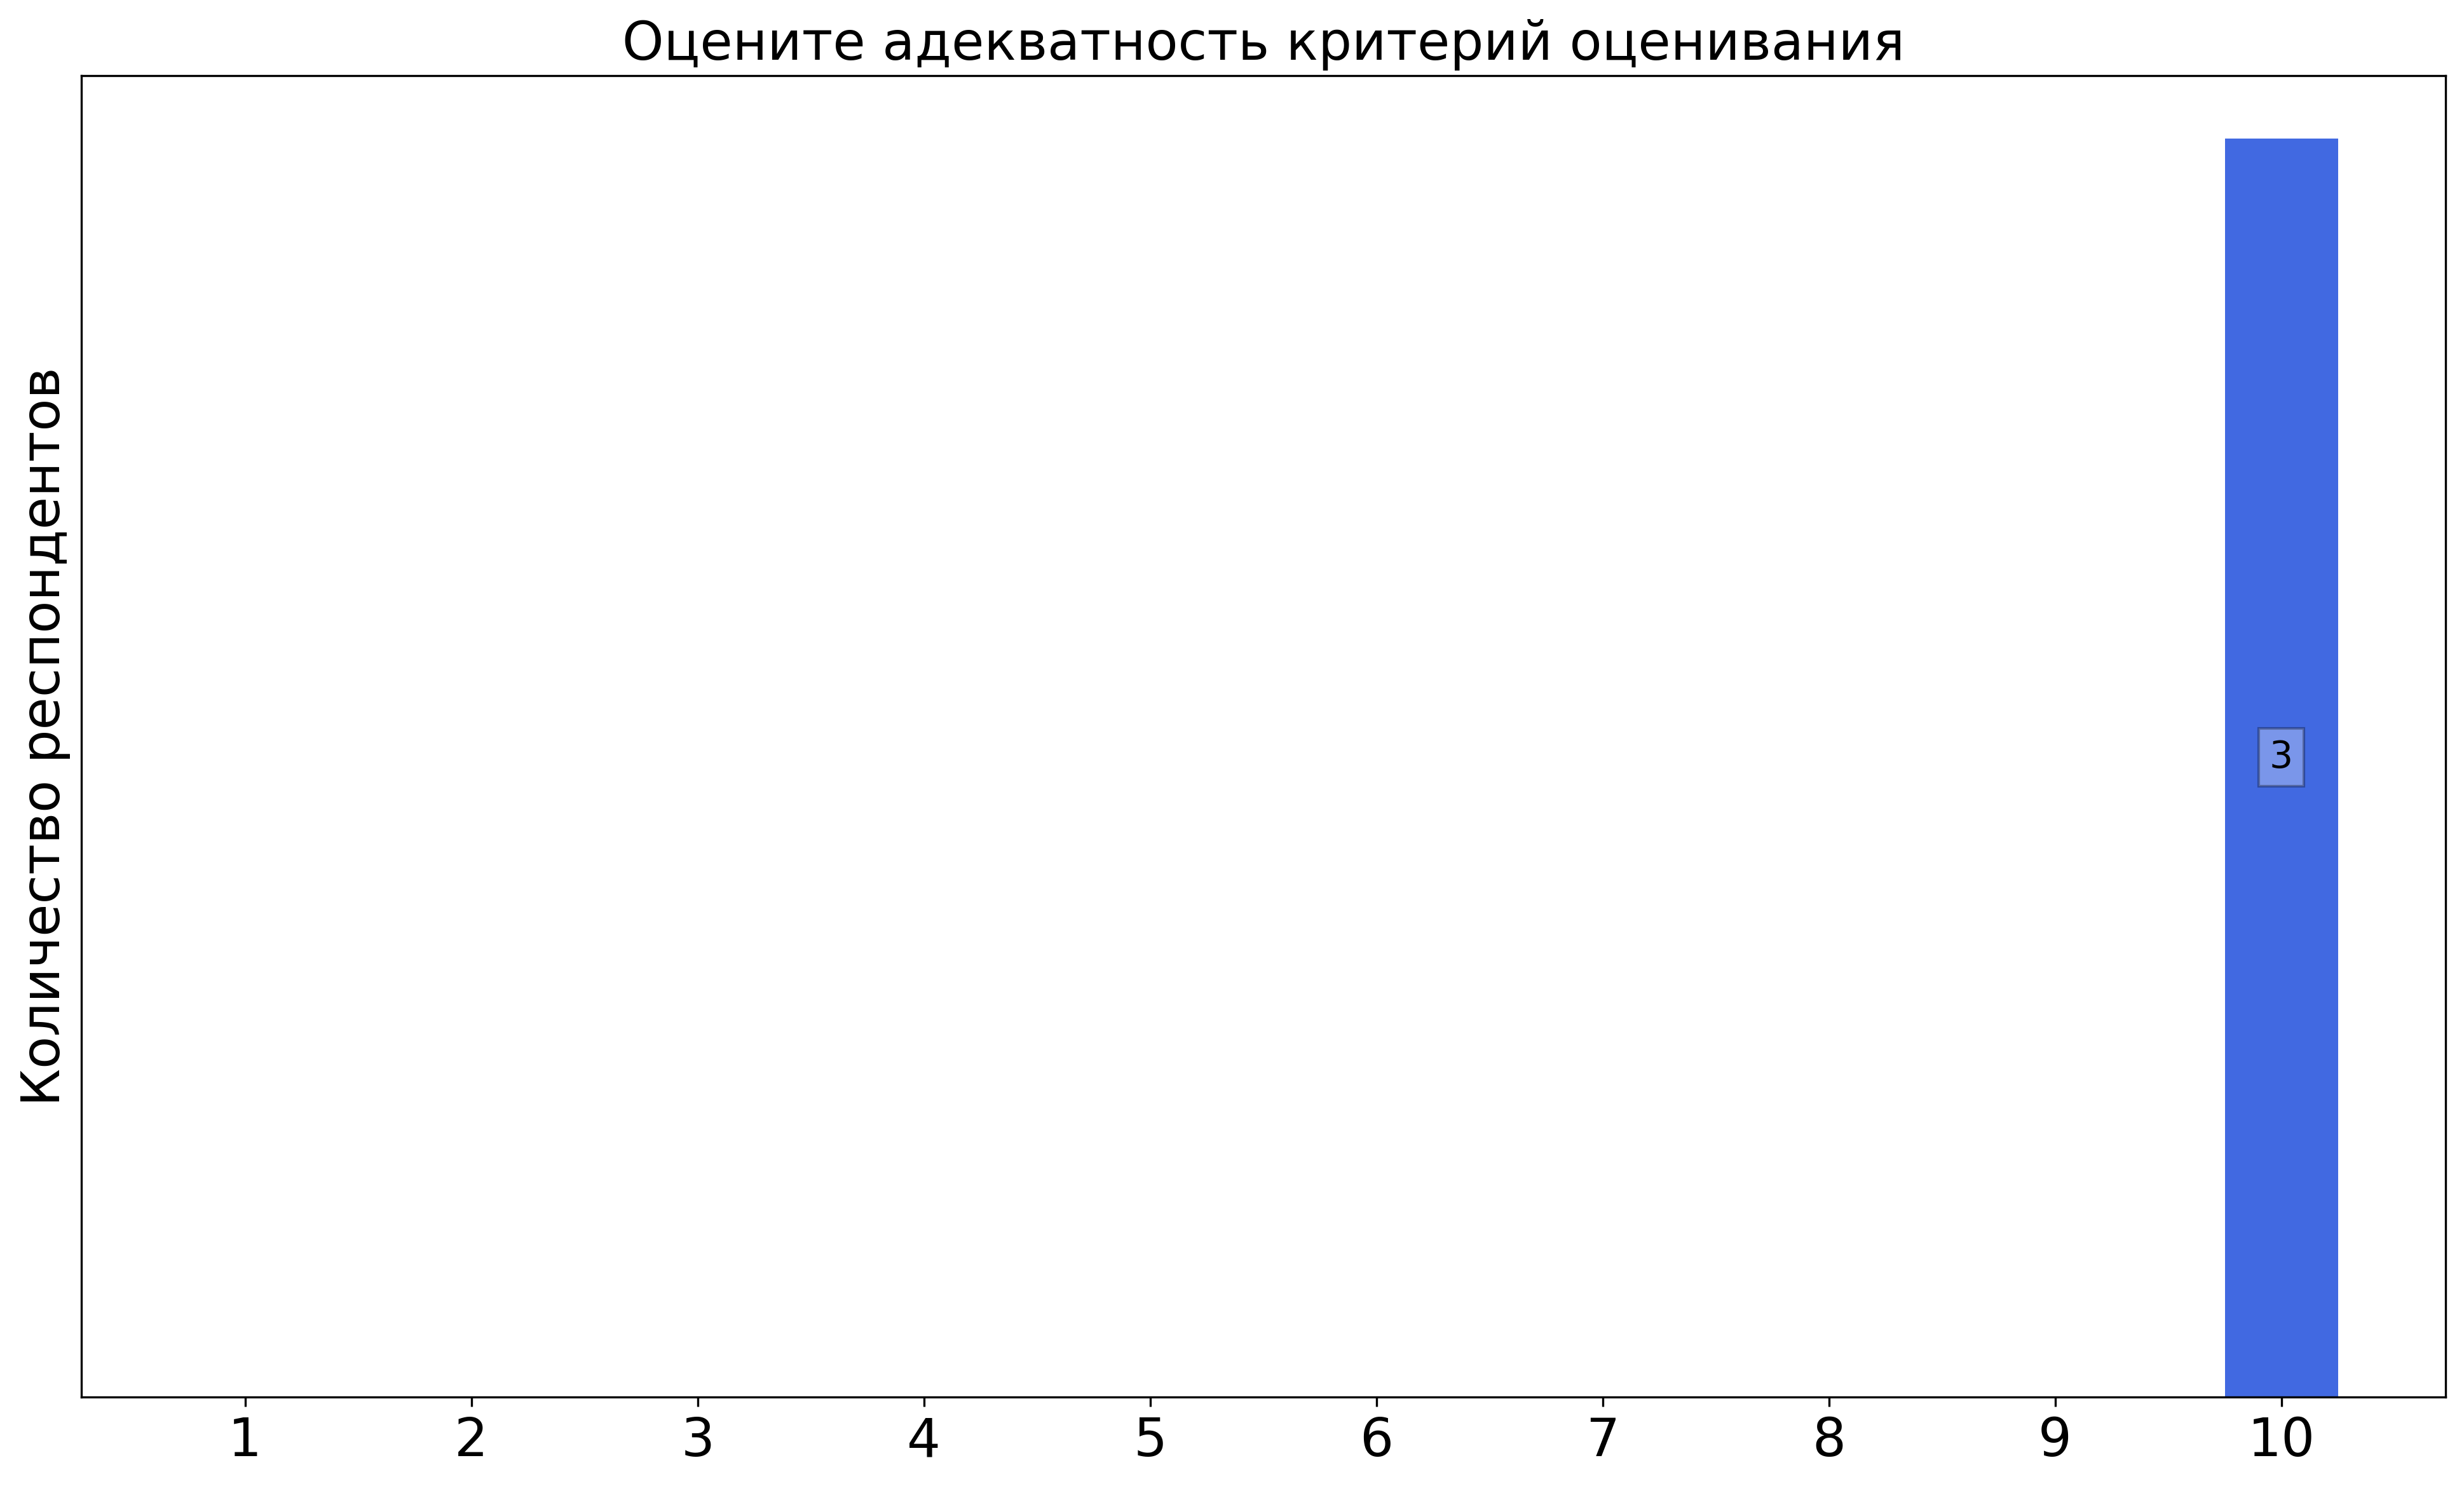
\includegraphics[width=\textwidth]{images/2 course/Аналитическая механика/seminarists-marks-Ахлумади Махди Реза-3.png}
            \end{subfigure}	
            \caption{Оценки респондентов о качестве преподавания семинаров}
        \end{figure}


    \subsubsection{Отзыв студентов о семинарах. Семинарист: Маштаков Я.В.}
		\begin{figure}[H]
			\centering
			\begin{subfigure}[b]{0.45\textwidth}
				\centering
				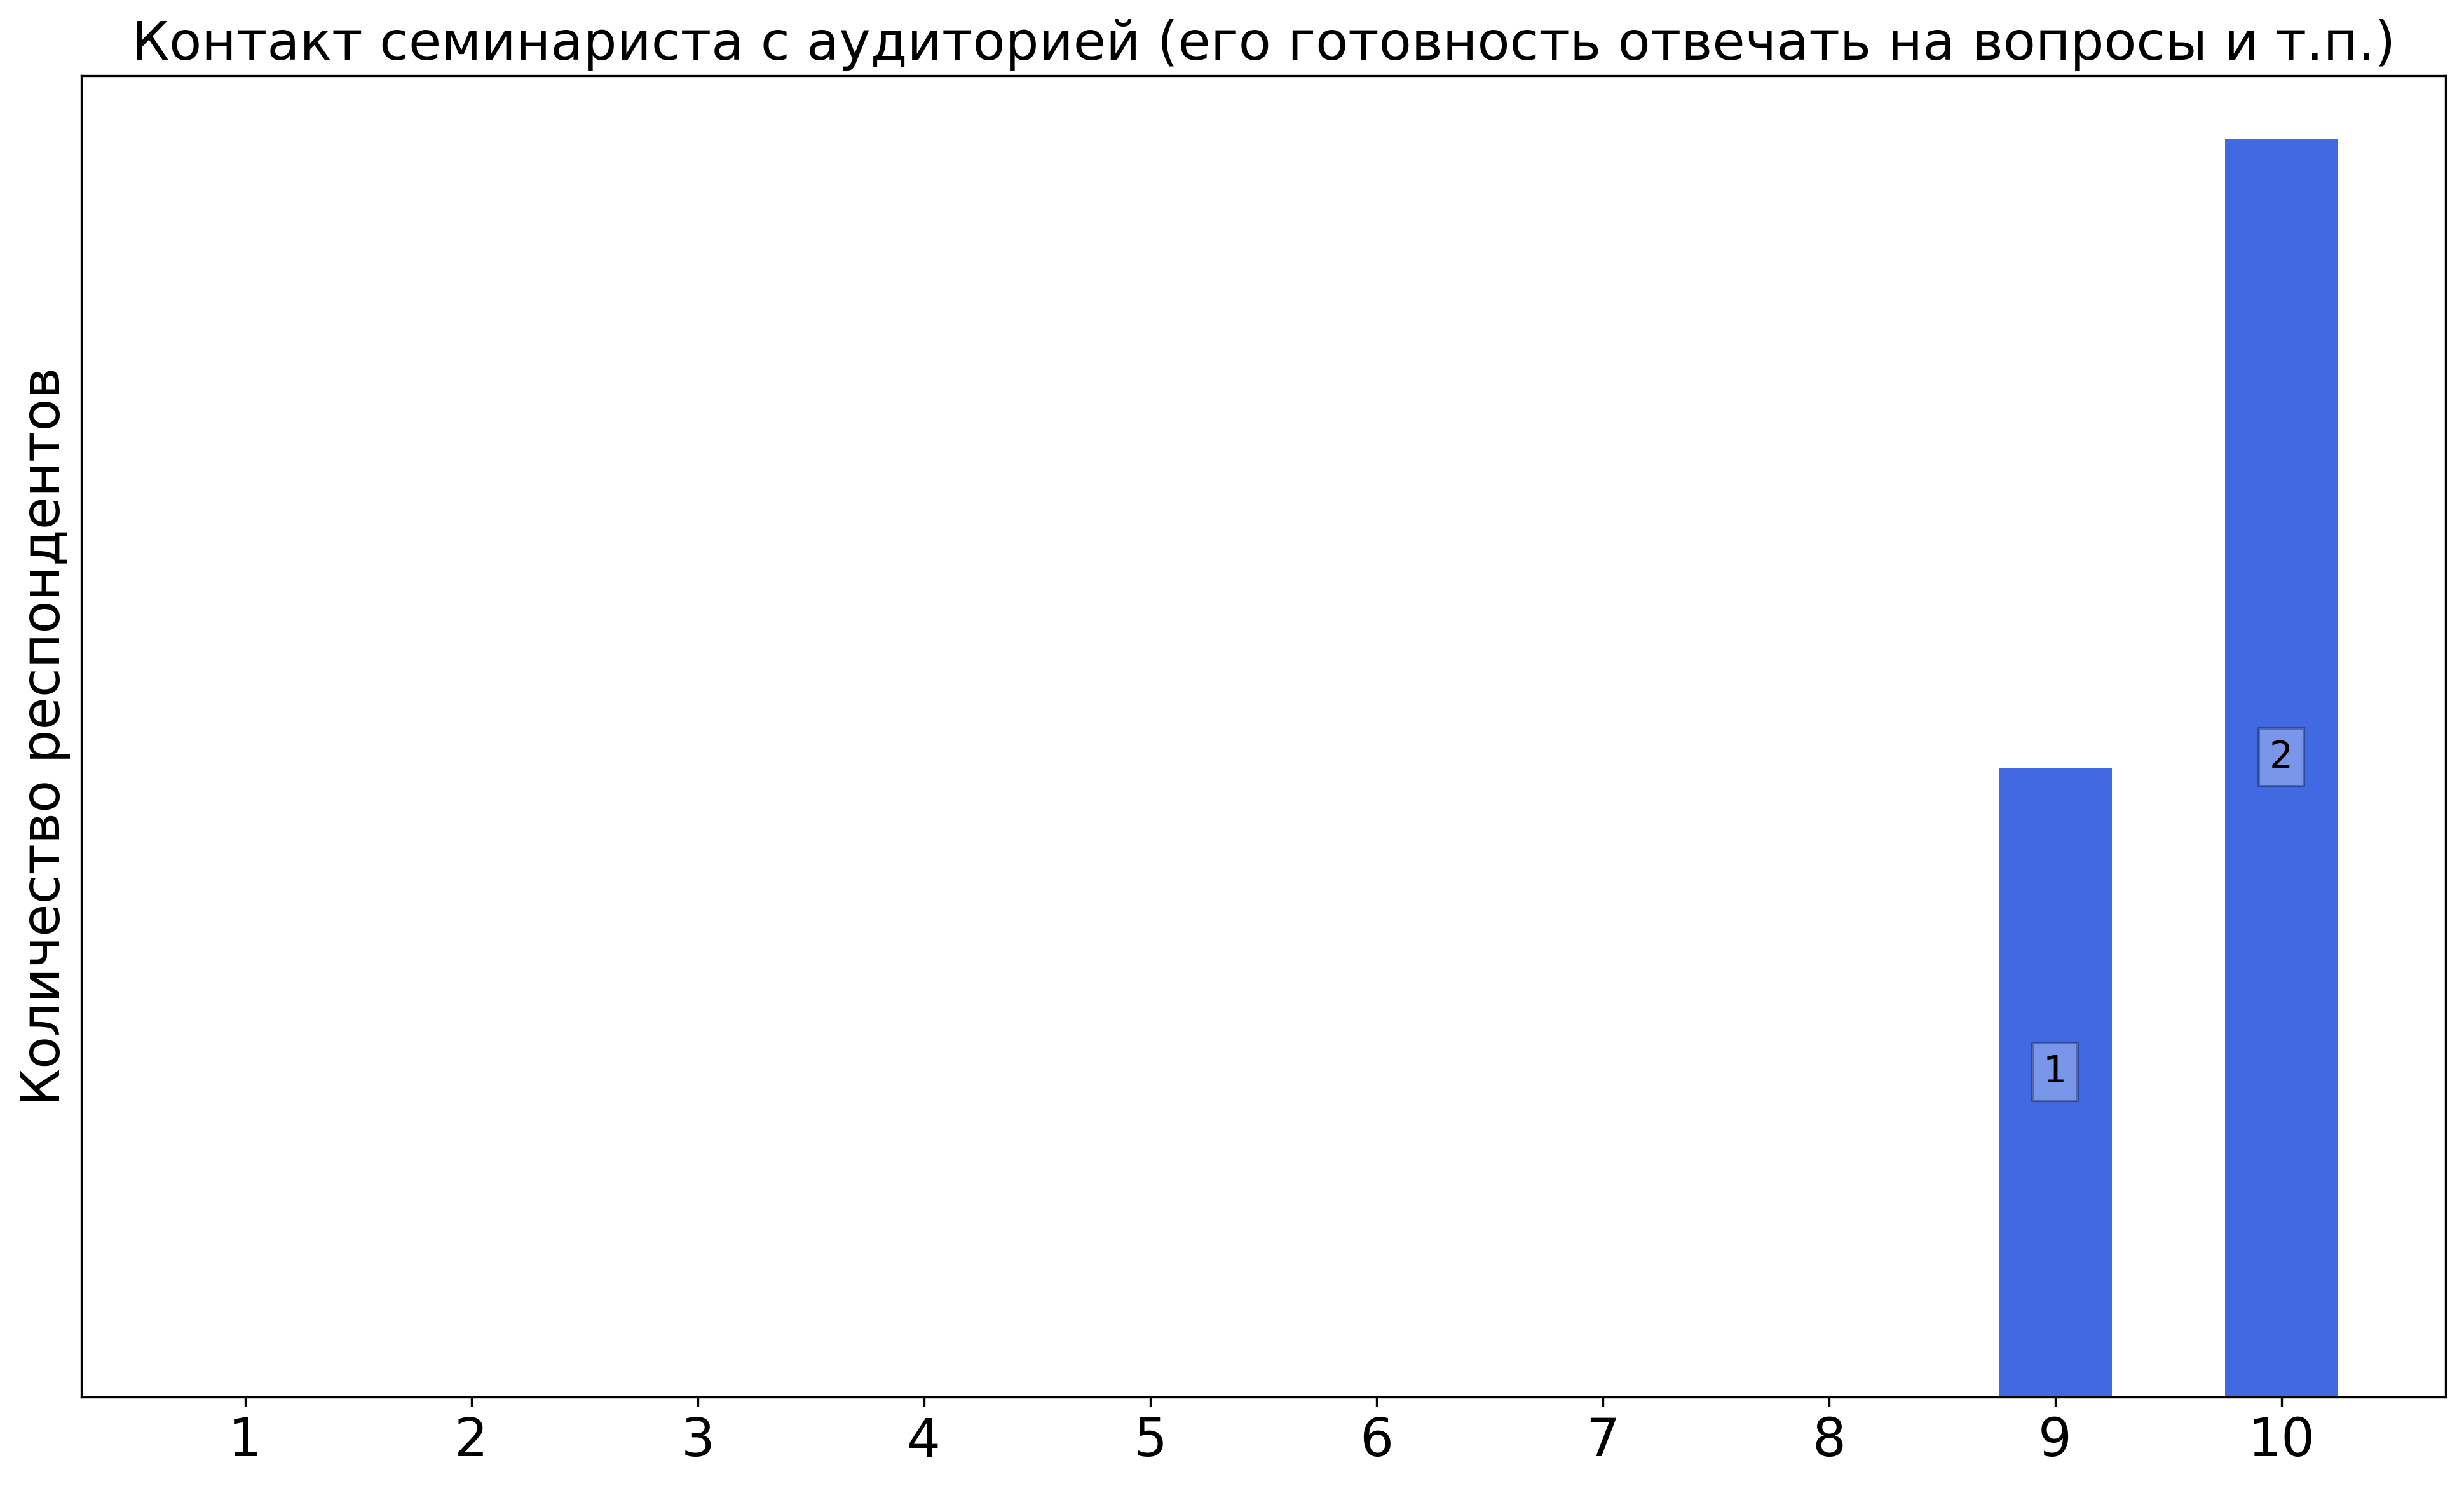
\includegraphics[width=\textwidth]{images/2 course/Аналитическая механика/seminarists-marks-Маштаков Я.В.-0.png}
			\end{subfigure}
			\begin{subfigure}[b]{0.45\textwidth}
				\centering
				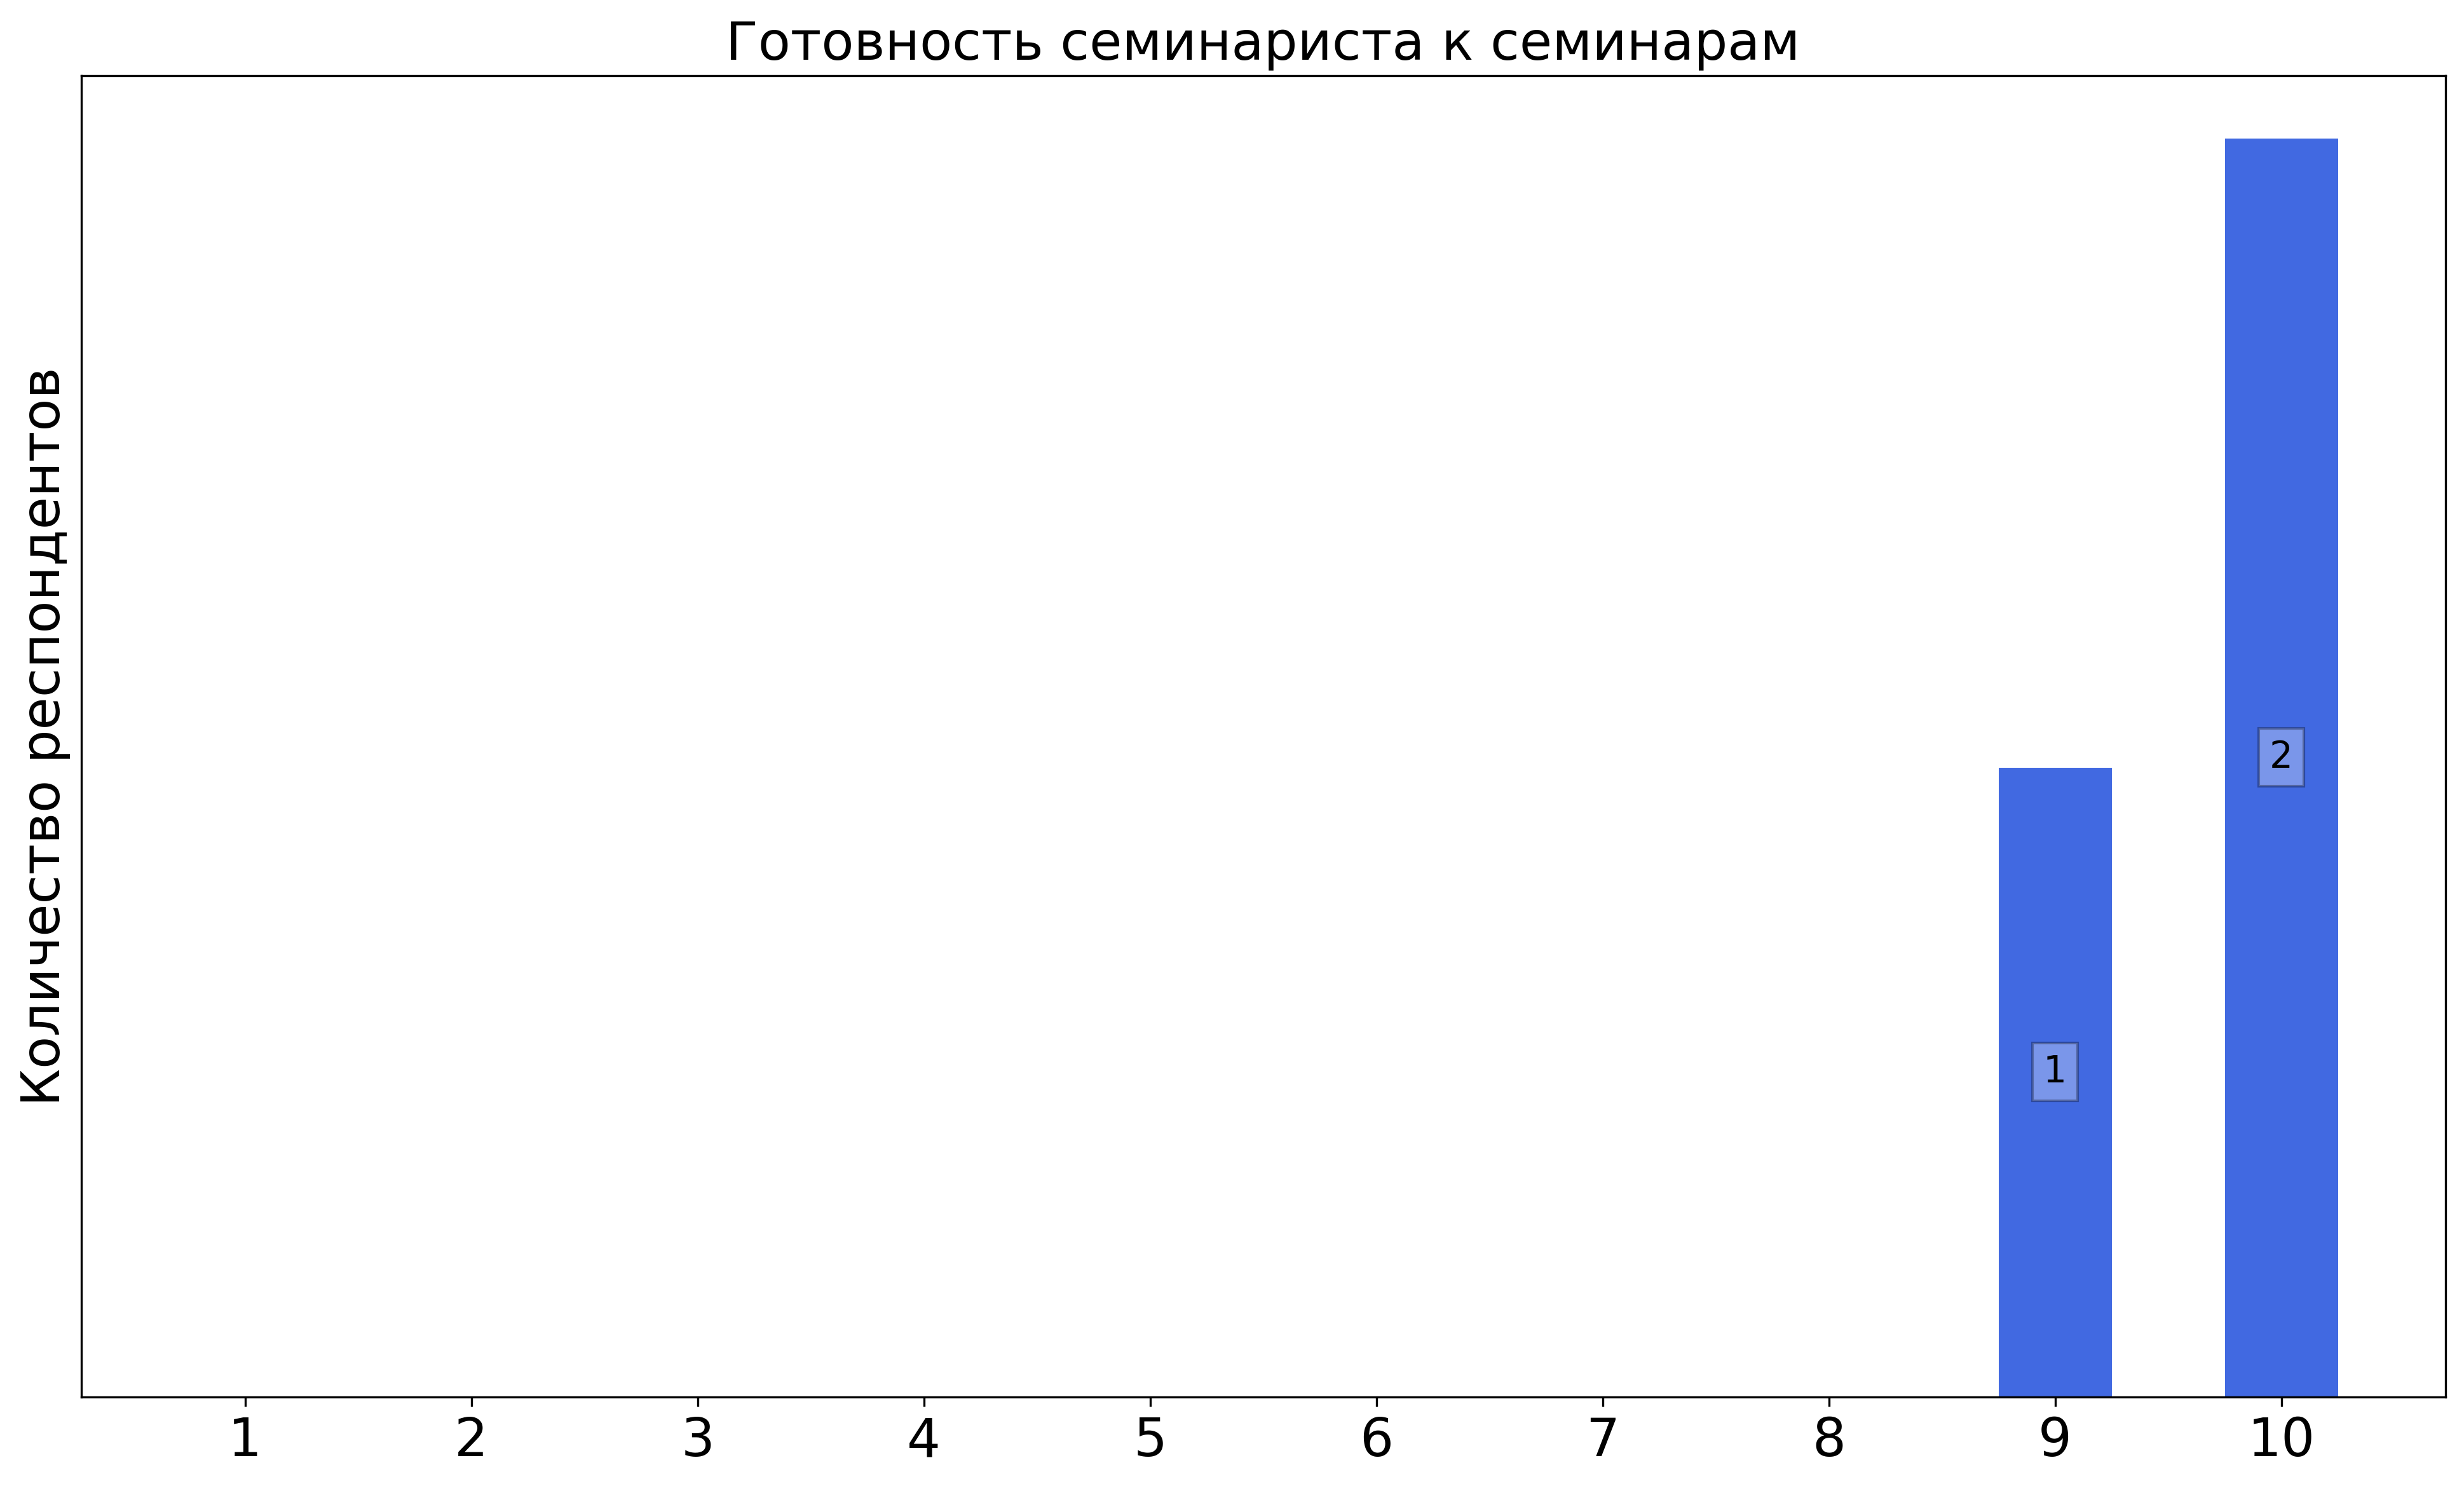
\includegraphics[width=\textwidth]{images/2 course/Аналитическая механика/seminarists-marks-Маштаков Я.В.-1.png}
			\end{subfigure}
			\begin{subfigure}[b]{0.45\textwidth}
				\centering
				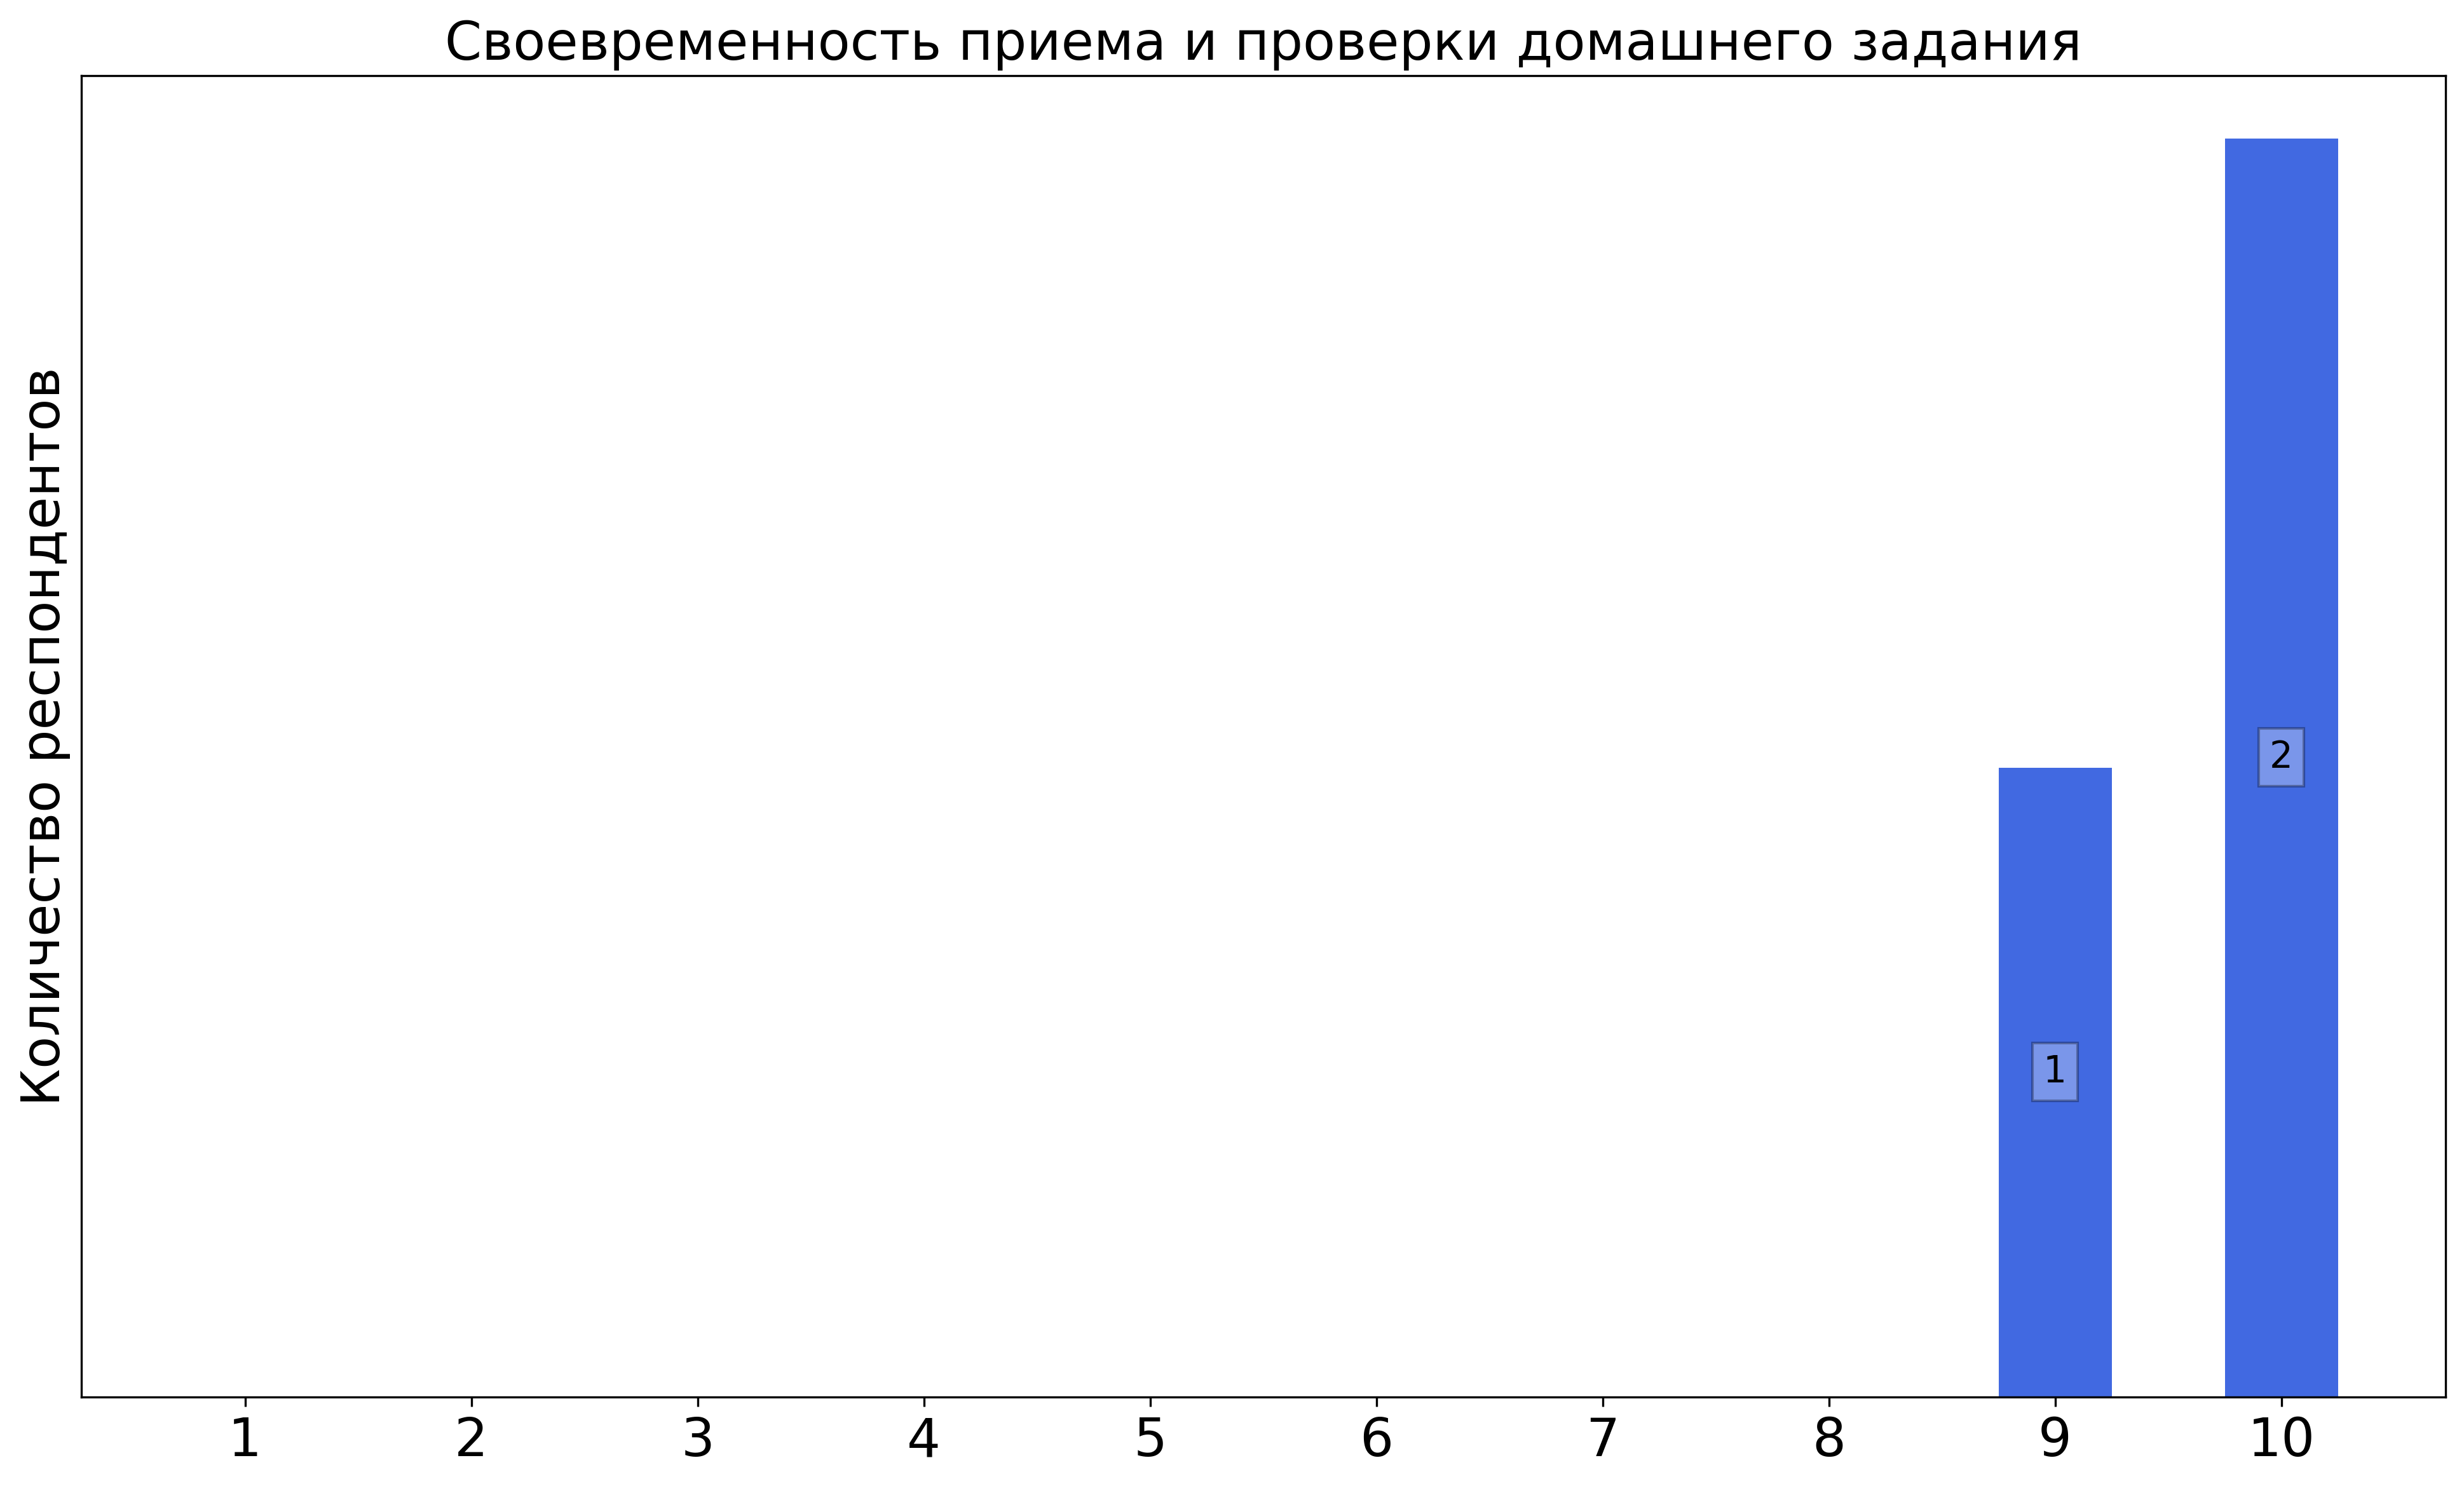
\includegraphics[width=\textwidth]{images/2 course/Аналитическая механика/seminarists-marks-Маштаков Я.В.-2.png}
			\end{subfigure}
			\begin{subfigure}[b]{0.45\textwidth}
				\centering
				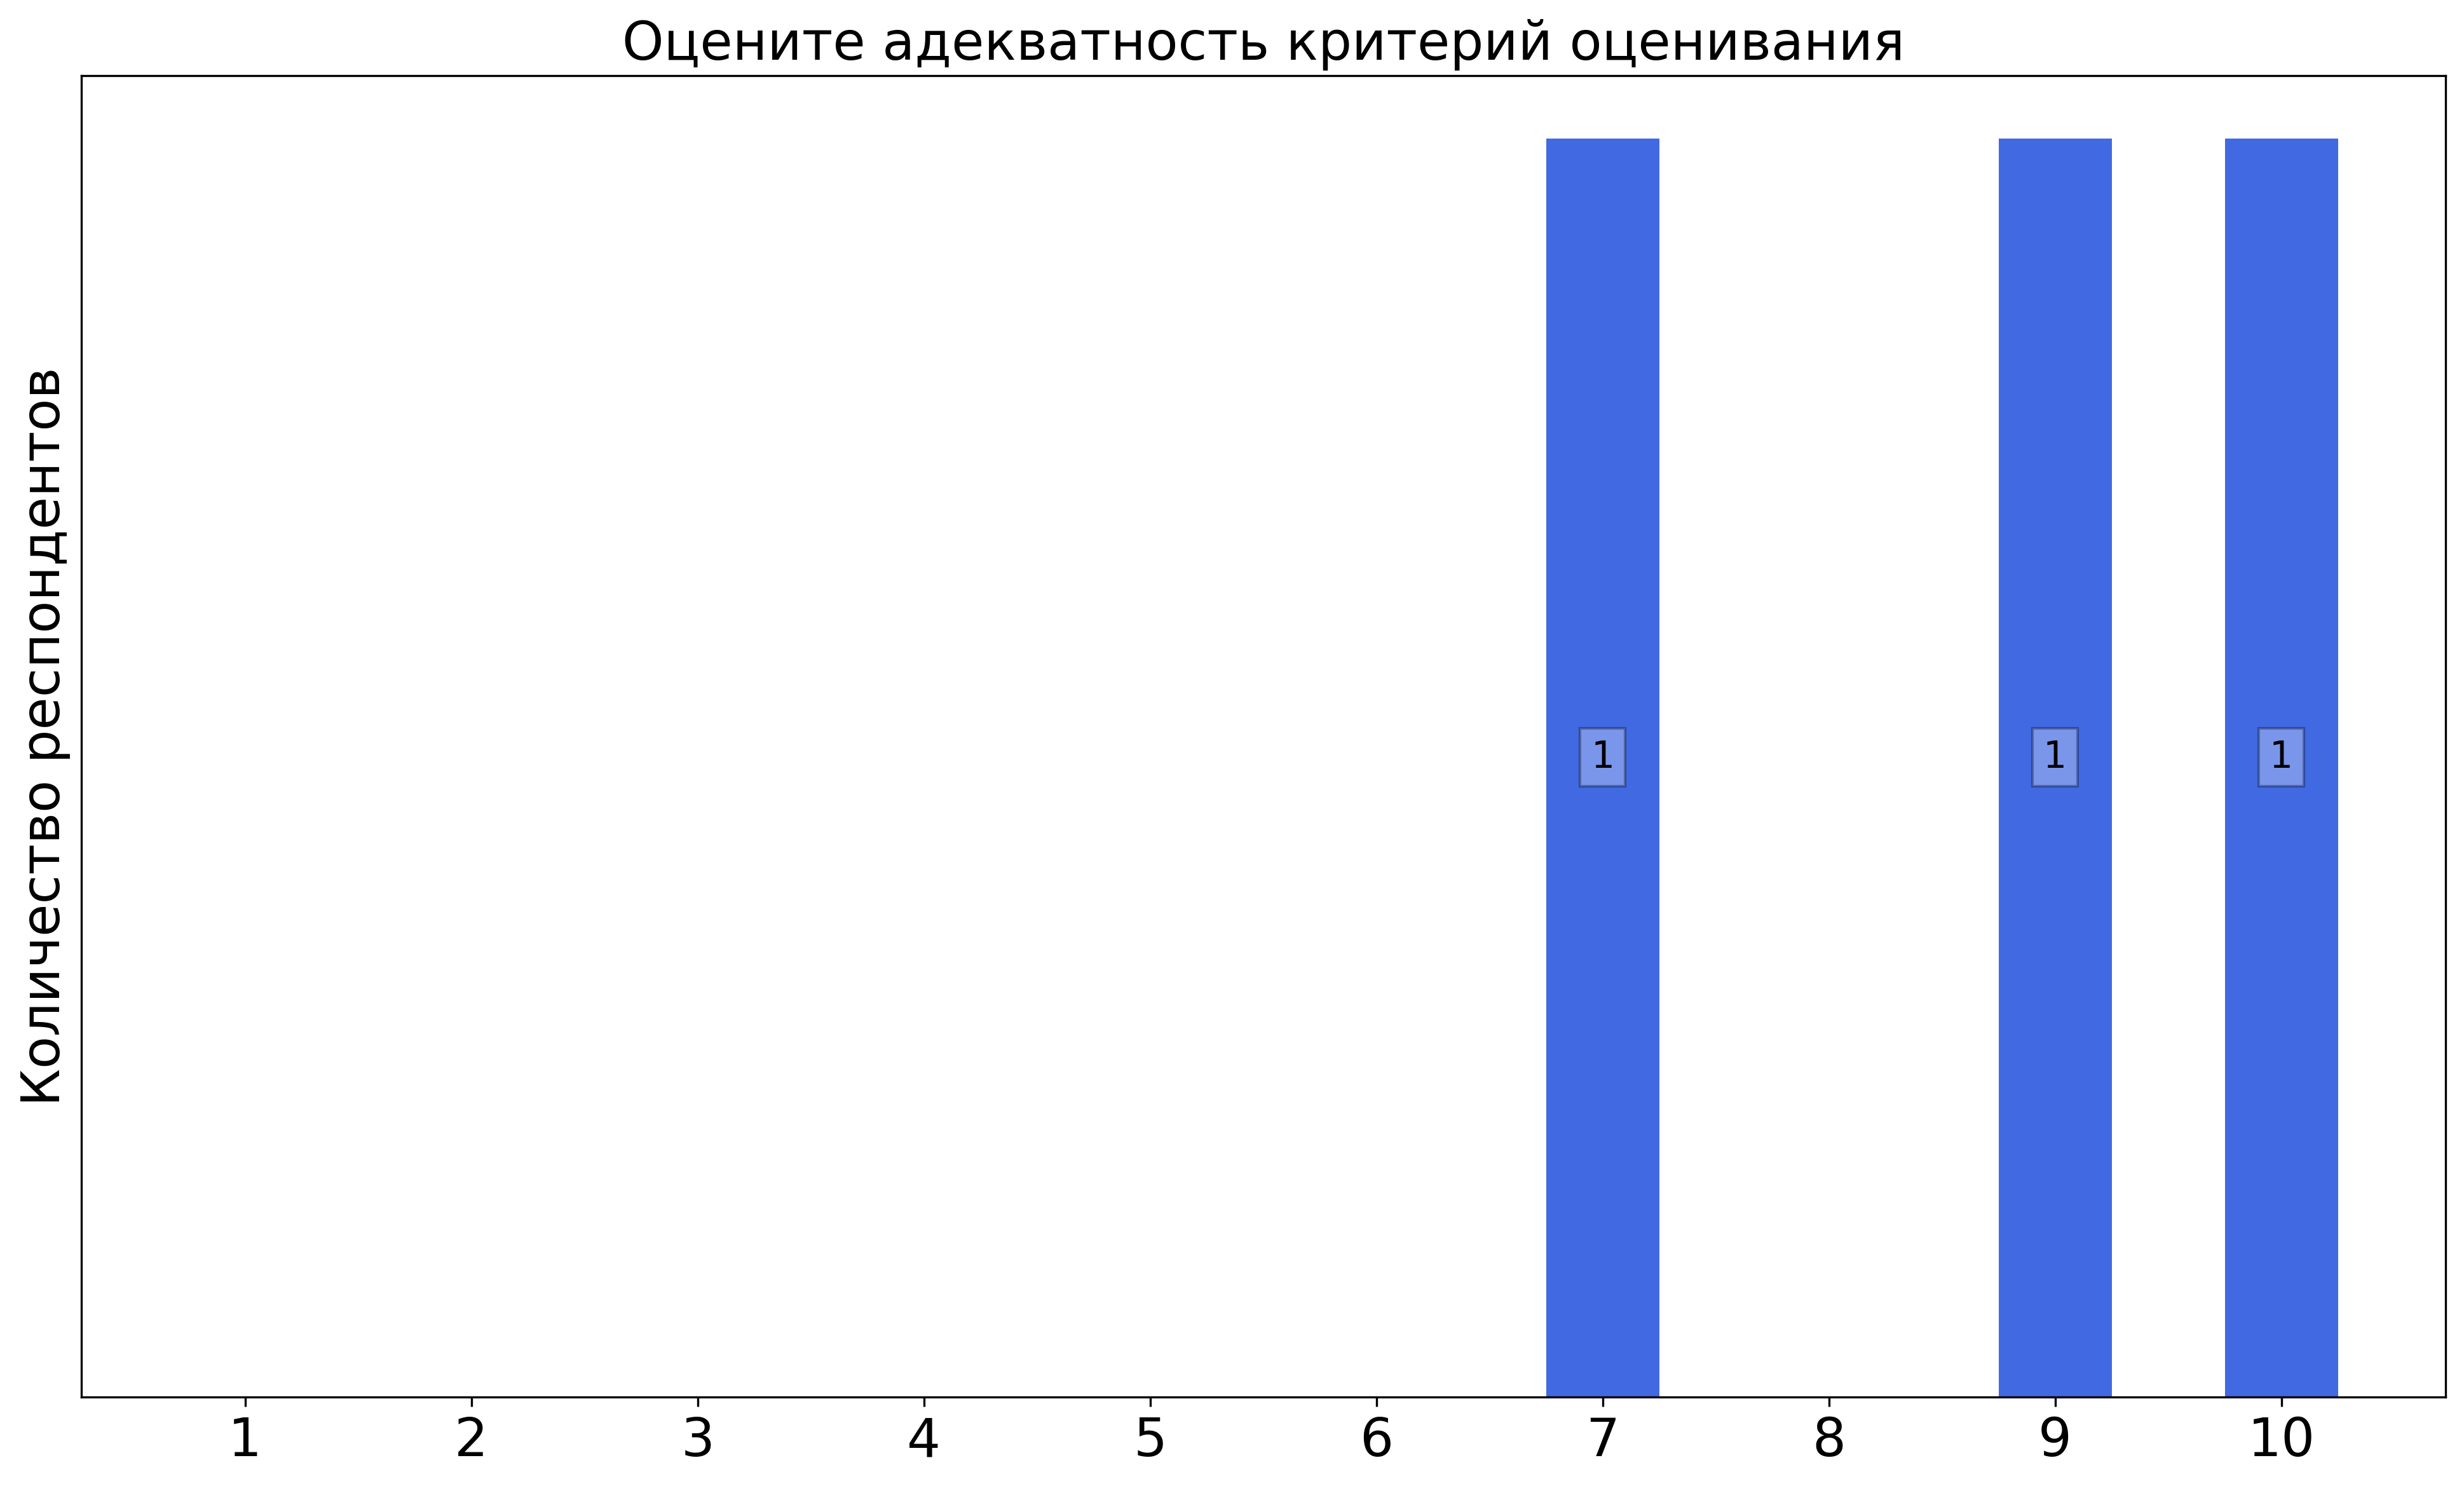
\includegraphics[width=\textwidth]{images/2 course/Аналитическая механика/seminarists-marks-Маштаков Я.В.-3.png}
			\end{subfigure}	
			\caption{Оценки респондентов о качестве преподавания семинаров}
		\end{figure}


        
    \subsubsection{Отзыв студентов о семинарах. Семинарист: Монахова У.В.}
		\begin{figure}[H]
			\centering
			\begin{subfigure}[b]{0.45\textwidth}
				\centering
				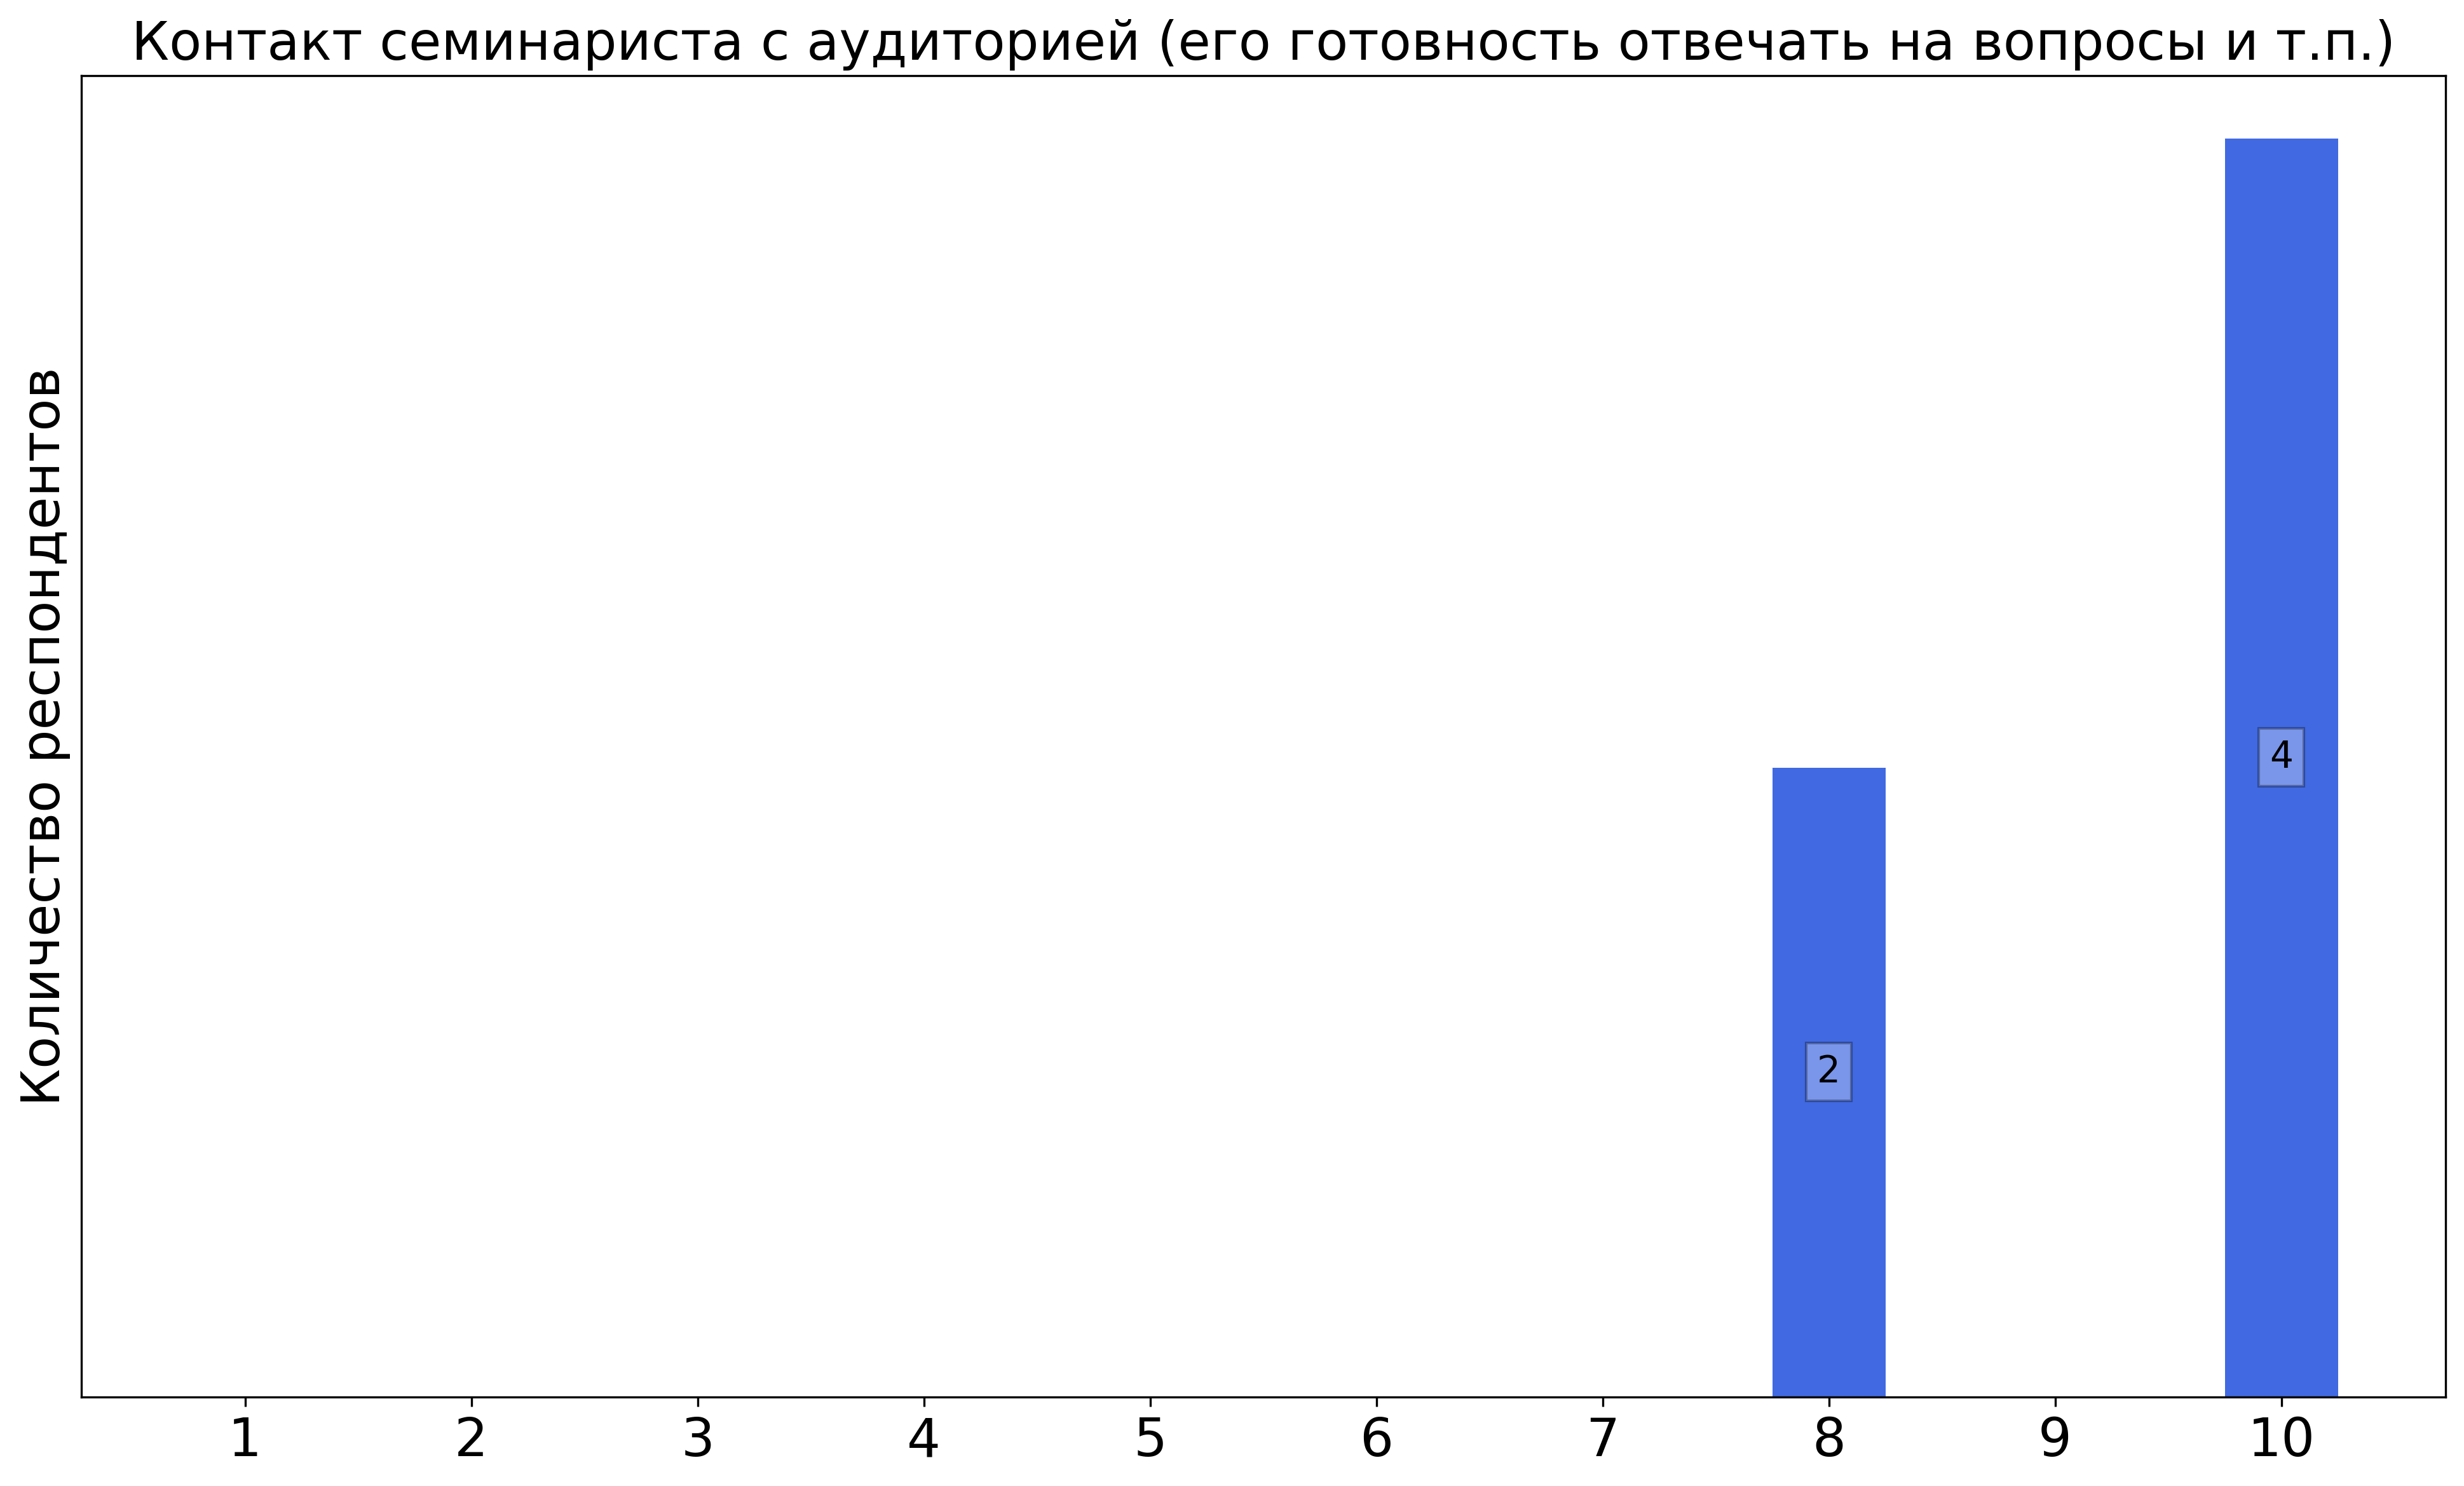
\includegraphics[width=\textwidth]{images/2 course/Аналитическая механика/seminarists-marks-Монахова У.В.-0.png}
			\end{subfigure}
			\begin{subfigure}[b]{0.45\textwidth}
				\centering
				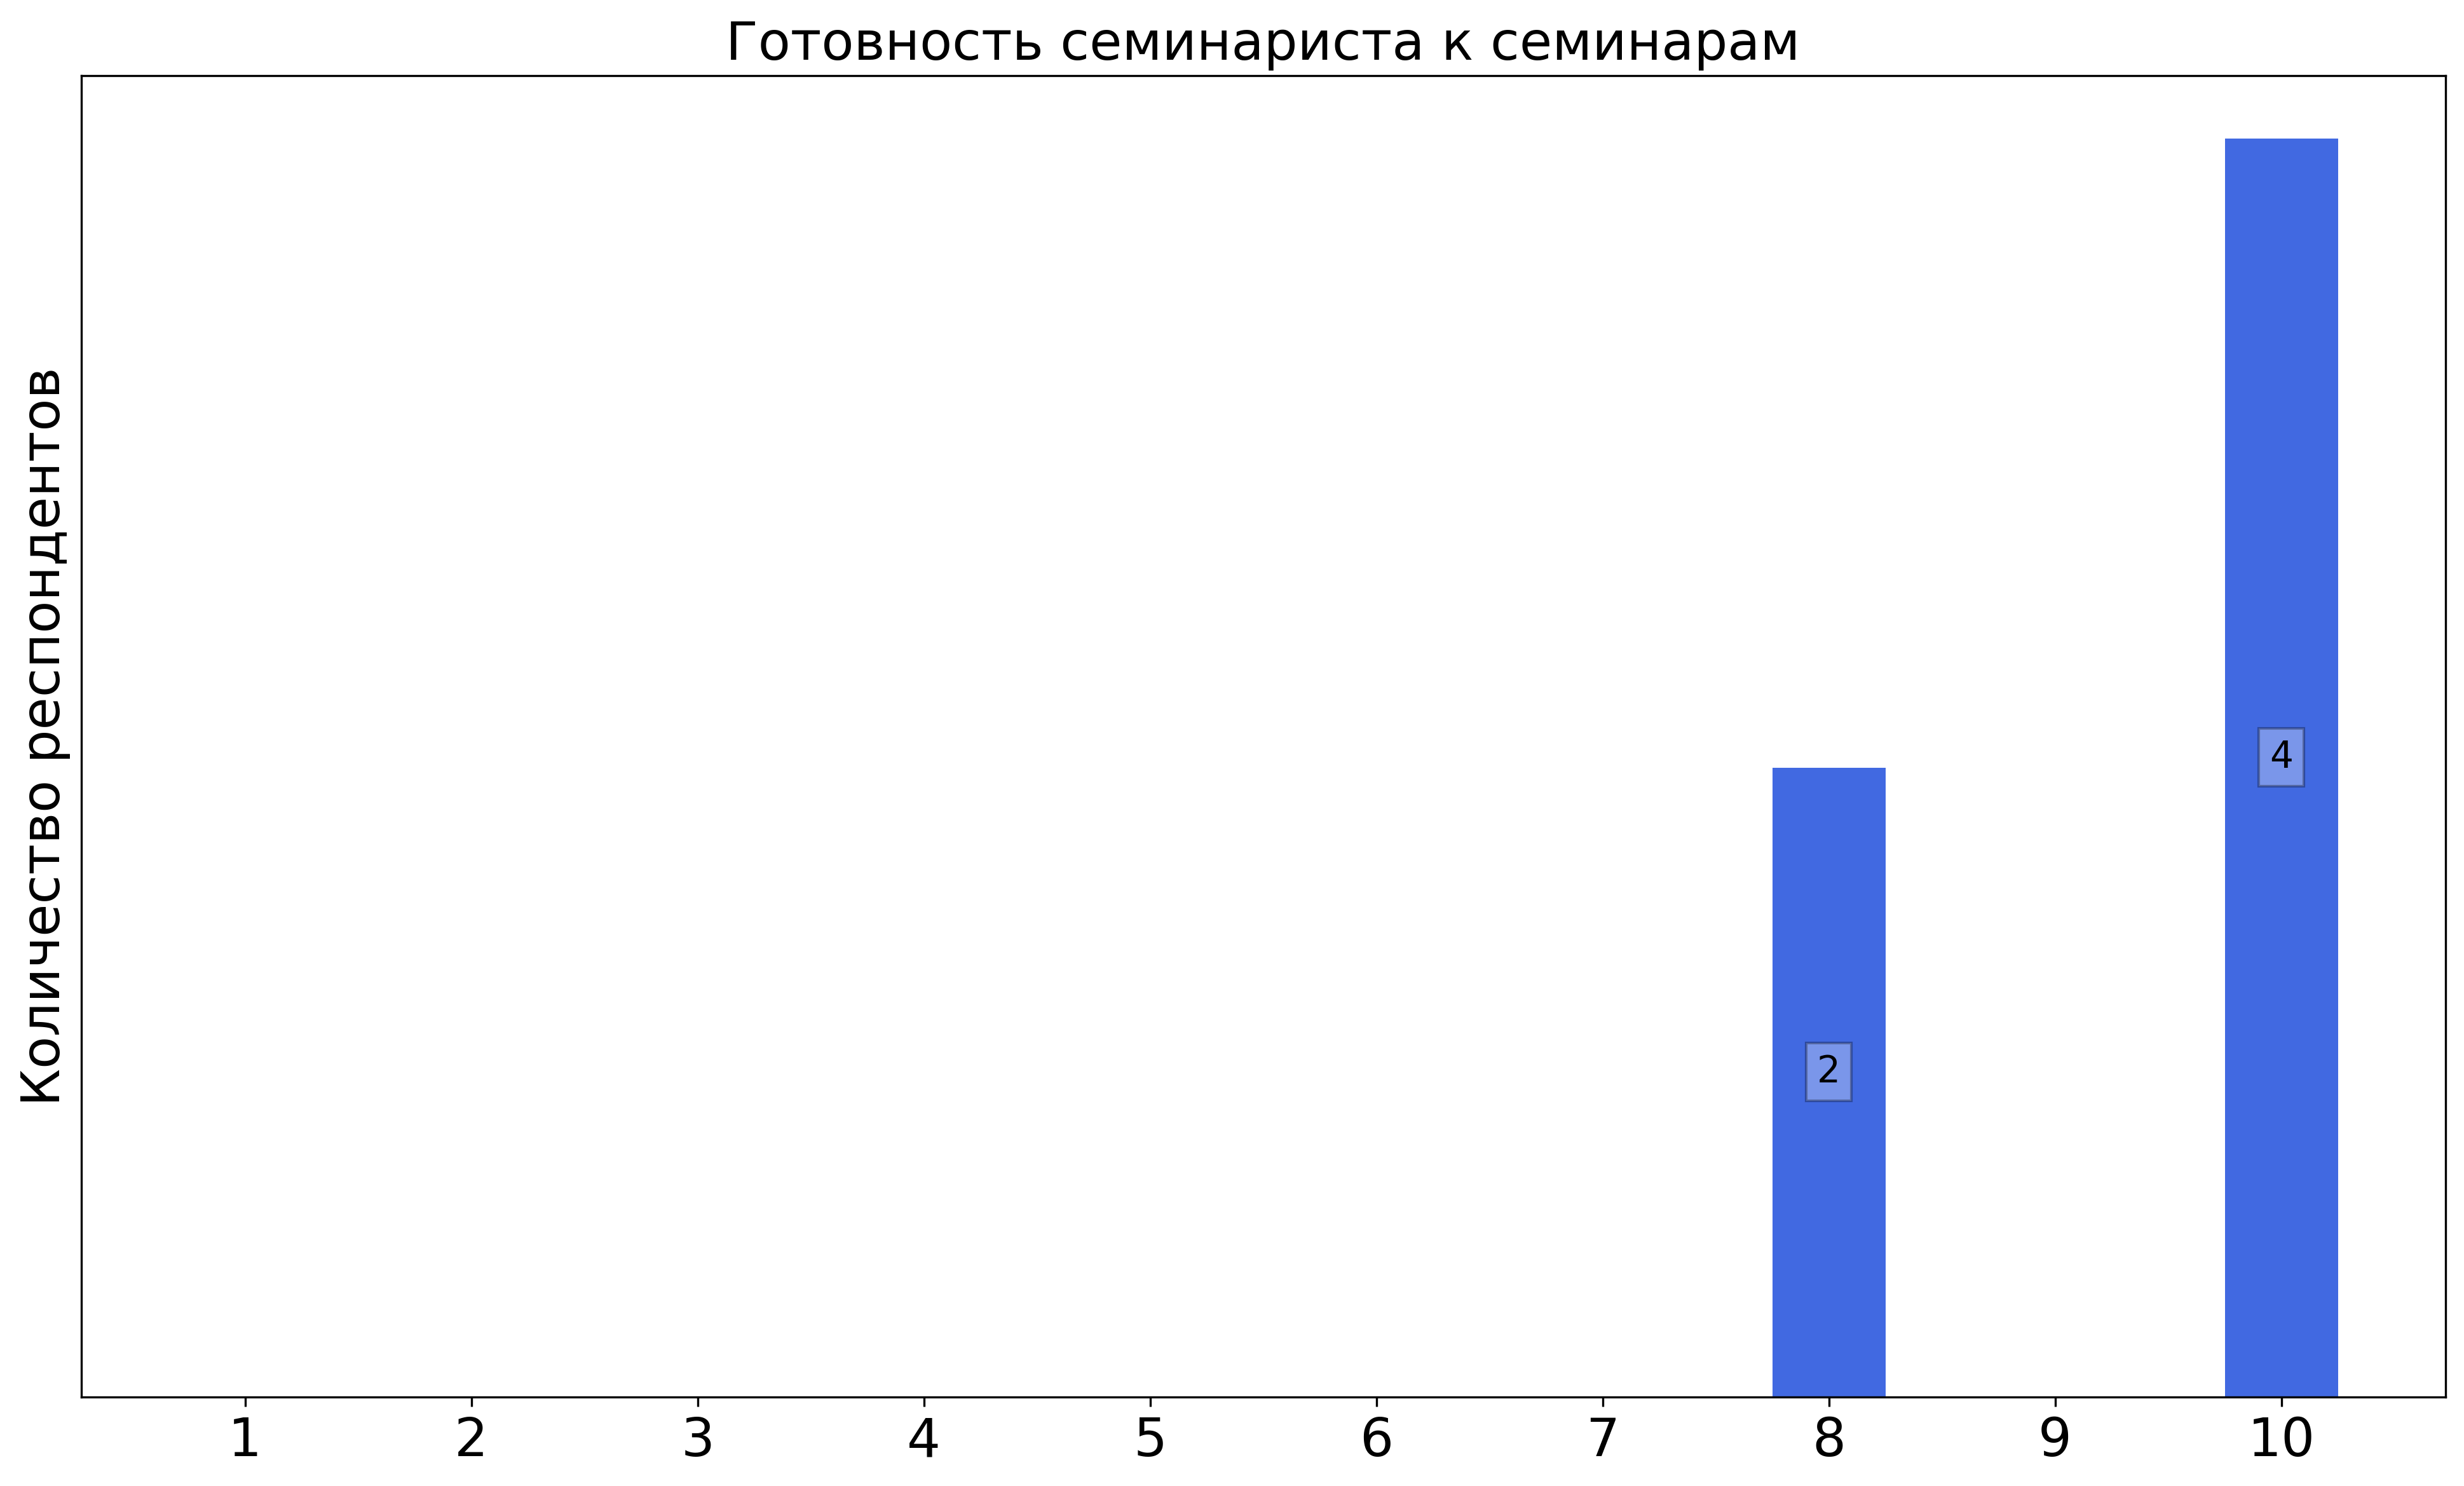
\includegraphics[width=\textwidth]{images/2 course/Аналитическая механика/seminarists-marks-Монахова У.В.-1.png}
			\end{subfigure}
			\begin{subfigure}[b]{0.45\textwidth}
				\centering
				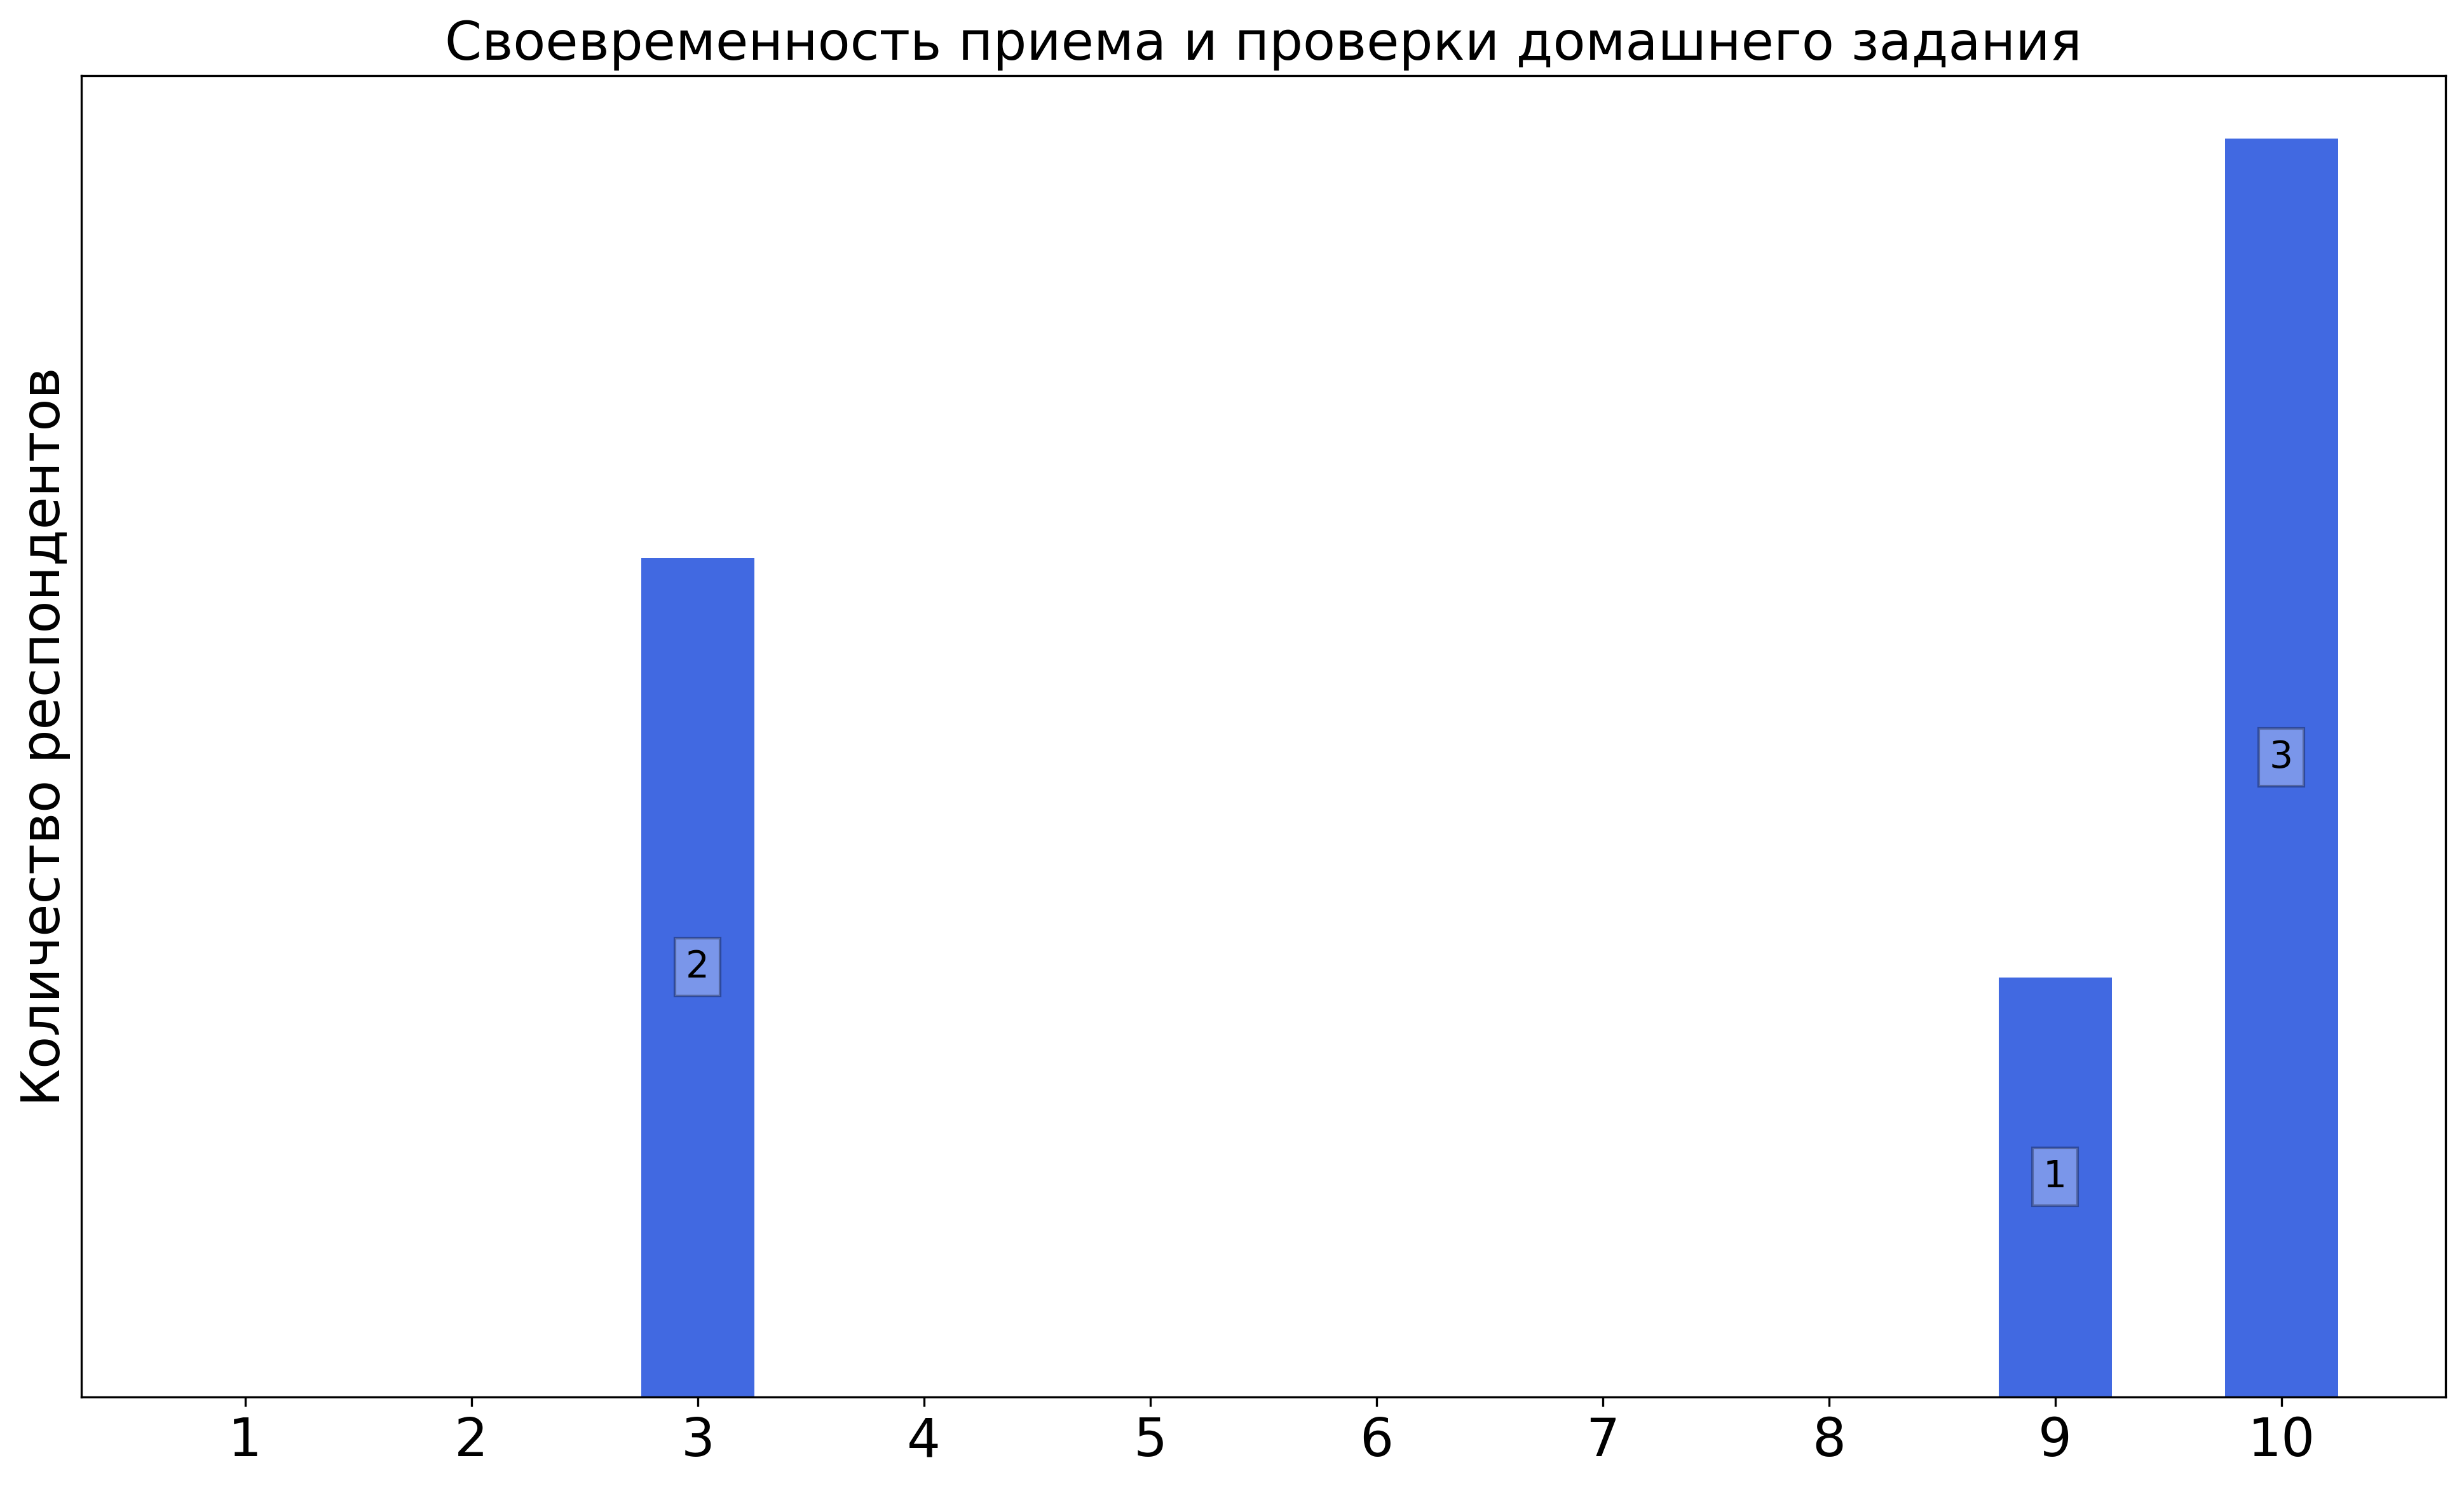
\includegraphics[width=\textwidth]{images/2 course/Аналитическая механика/seminarists-marks-Монахова У.В.-2.png}
			\end{subfigure}
			\begin{subfigure}[b]{0.45\textwidth}
				\centering
				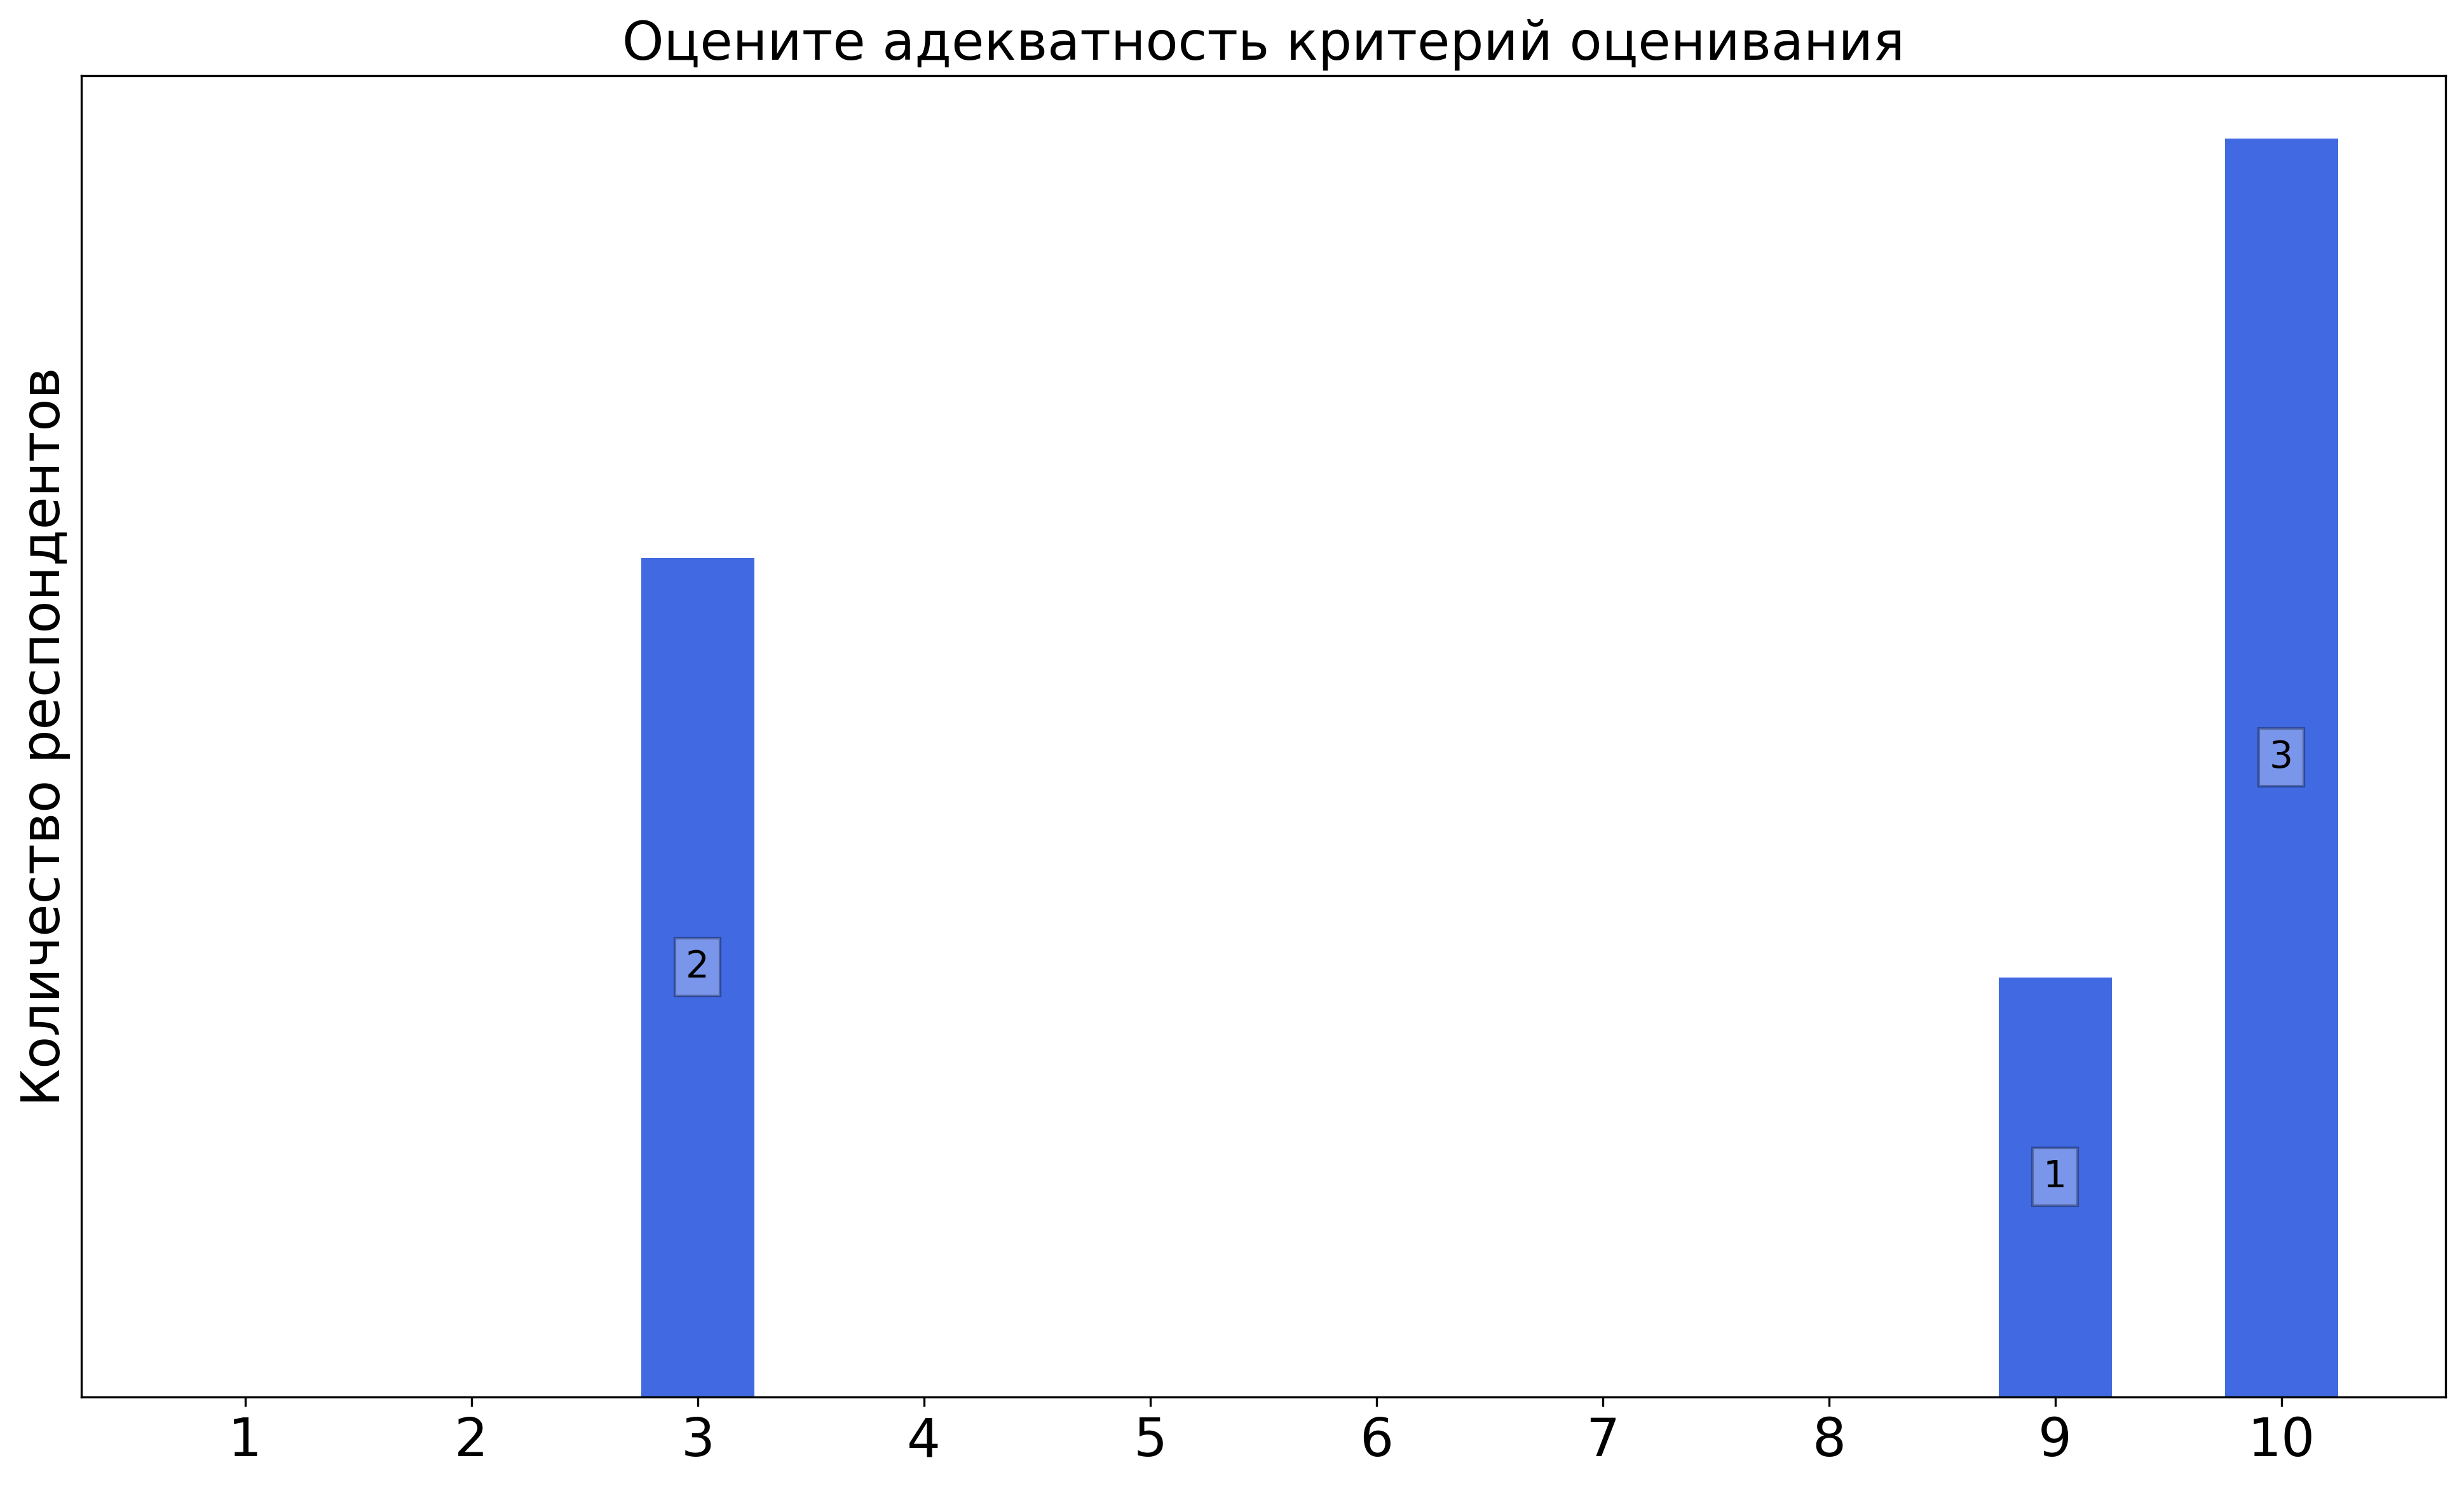
\includegraphics[width=\textwidth]{images/2 course/Аналитическая механика/seminarists-marks-Монахова У.В.-3.png}
			\end{subfigure}	
			\caption{Оценки респондентов о качестве преподавания семинаров}
		\end{figure}

		\textbf{Комментарии студентов о семинаристе\protect\footnote{сохранены оригинальные орфография и пунктуация}}
            \begin{commentbox} 
                Один из самых лучших преподаватель в МФТИ за всё время обучения
                Семинары понятные и интересные, домашнее задание решается легко после них
                Приятна в общении и всегда относится к студентам с любовью и уважением 
            \end{commentbox}


    \subsubsection{Отзыв студентов о семинарах. Семинарист: Сидоренко В.В.}
        \begin{figure}[H]
            \centering
            \begin{subfigure}[b]{0.45\textwidth}
                \centering
                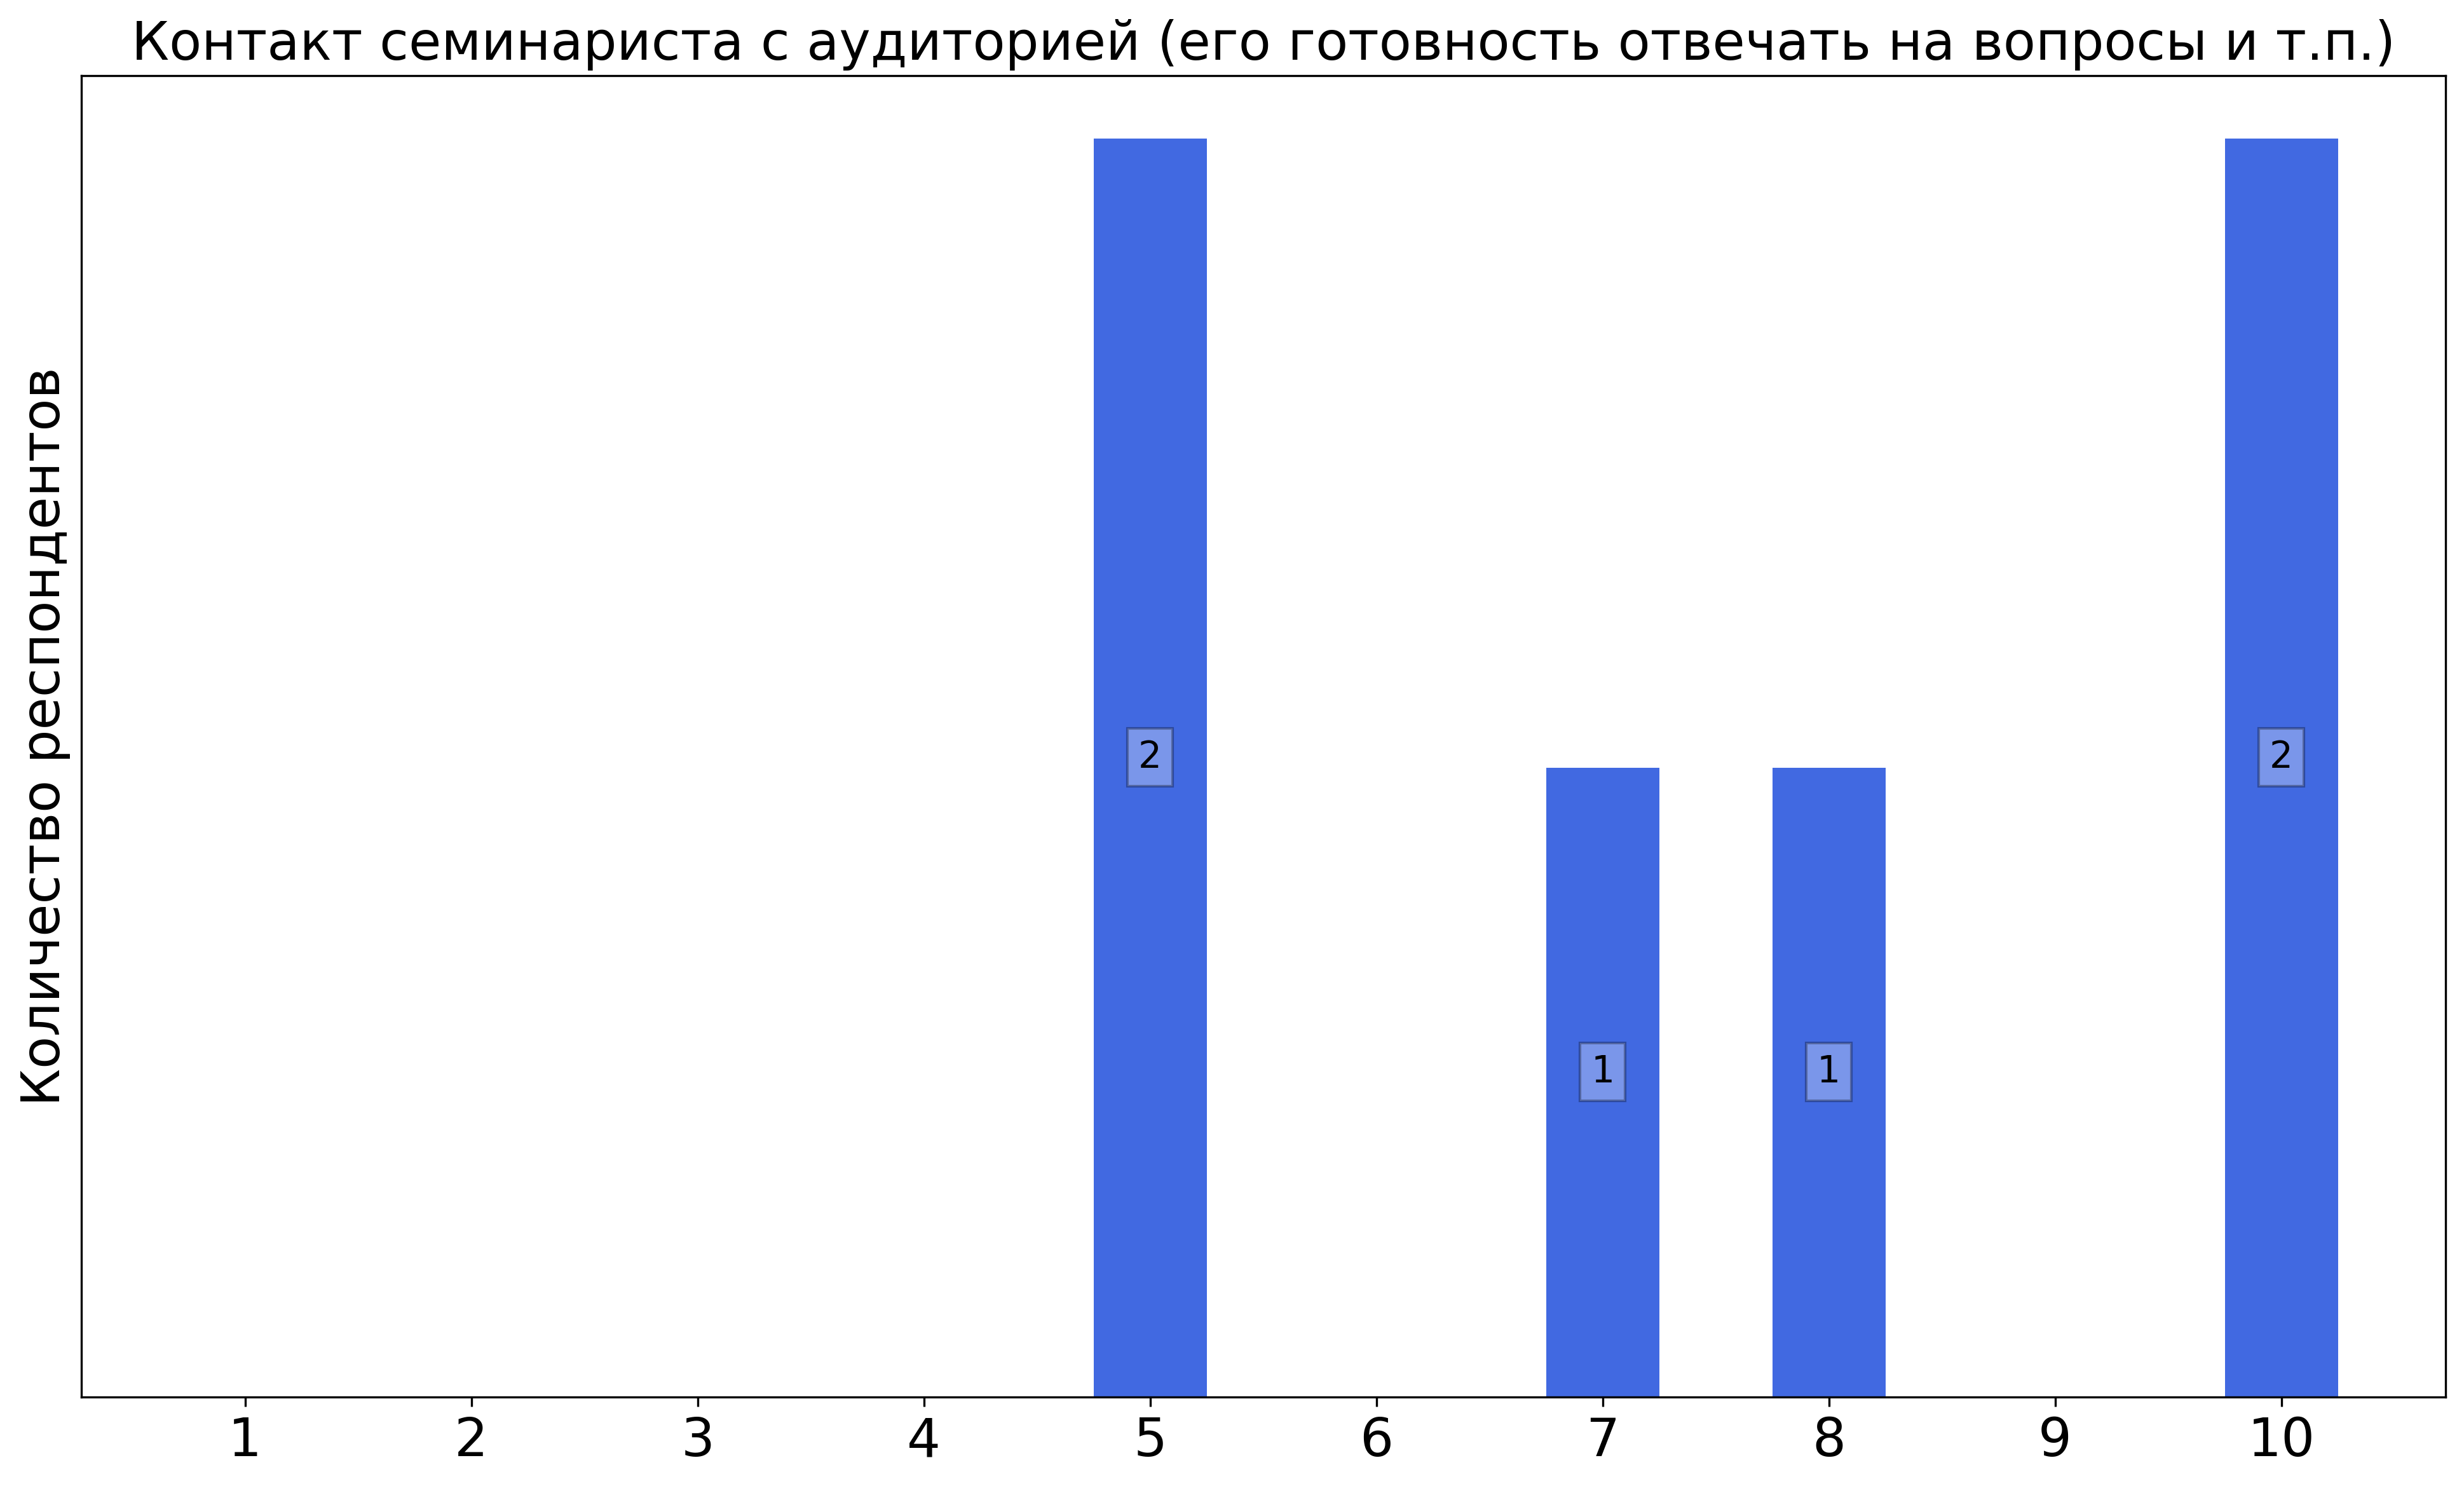
\includegraphics[width=\textwidth]{images/2 course/Аналитическая механика/seminarists-marks-Сидоренко В.В.-0.png}
            \end{subfigure}
            \begin{subfigure}[b]{0.45\textwidth}
                \centering
                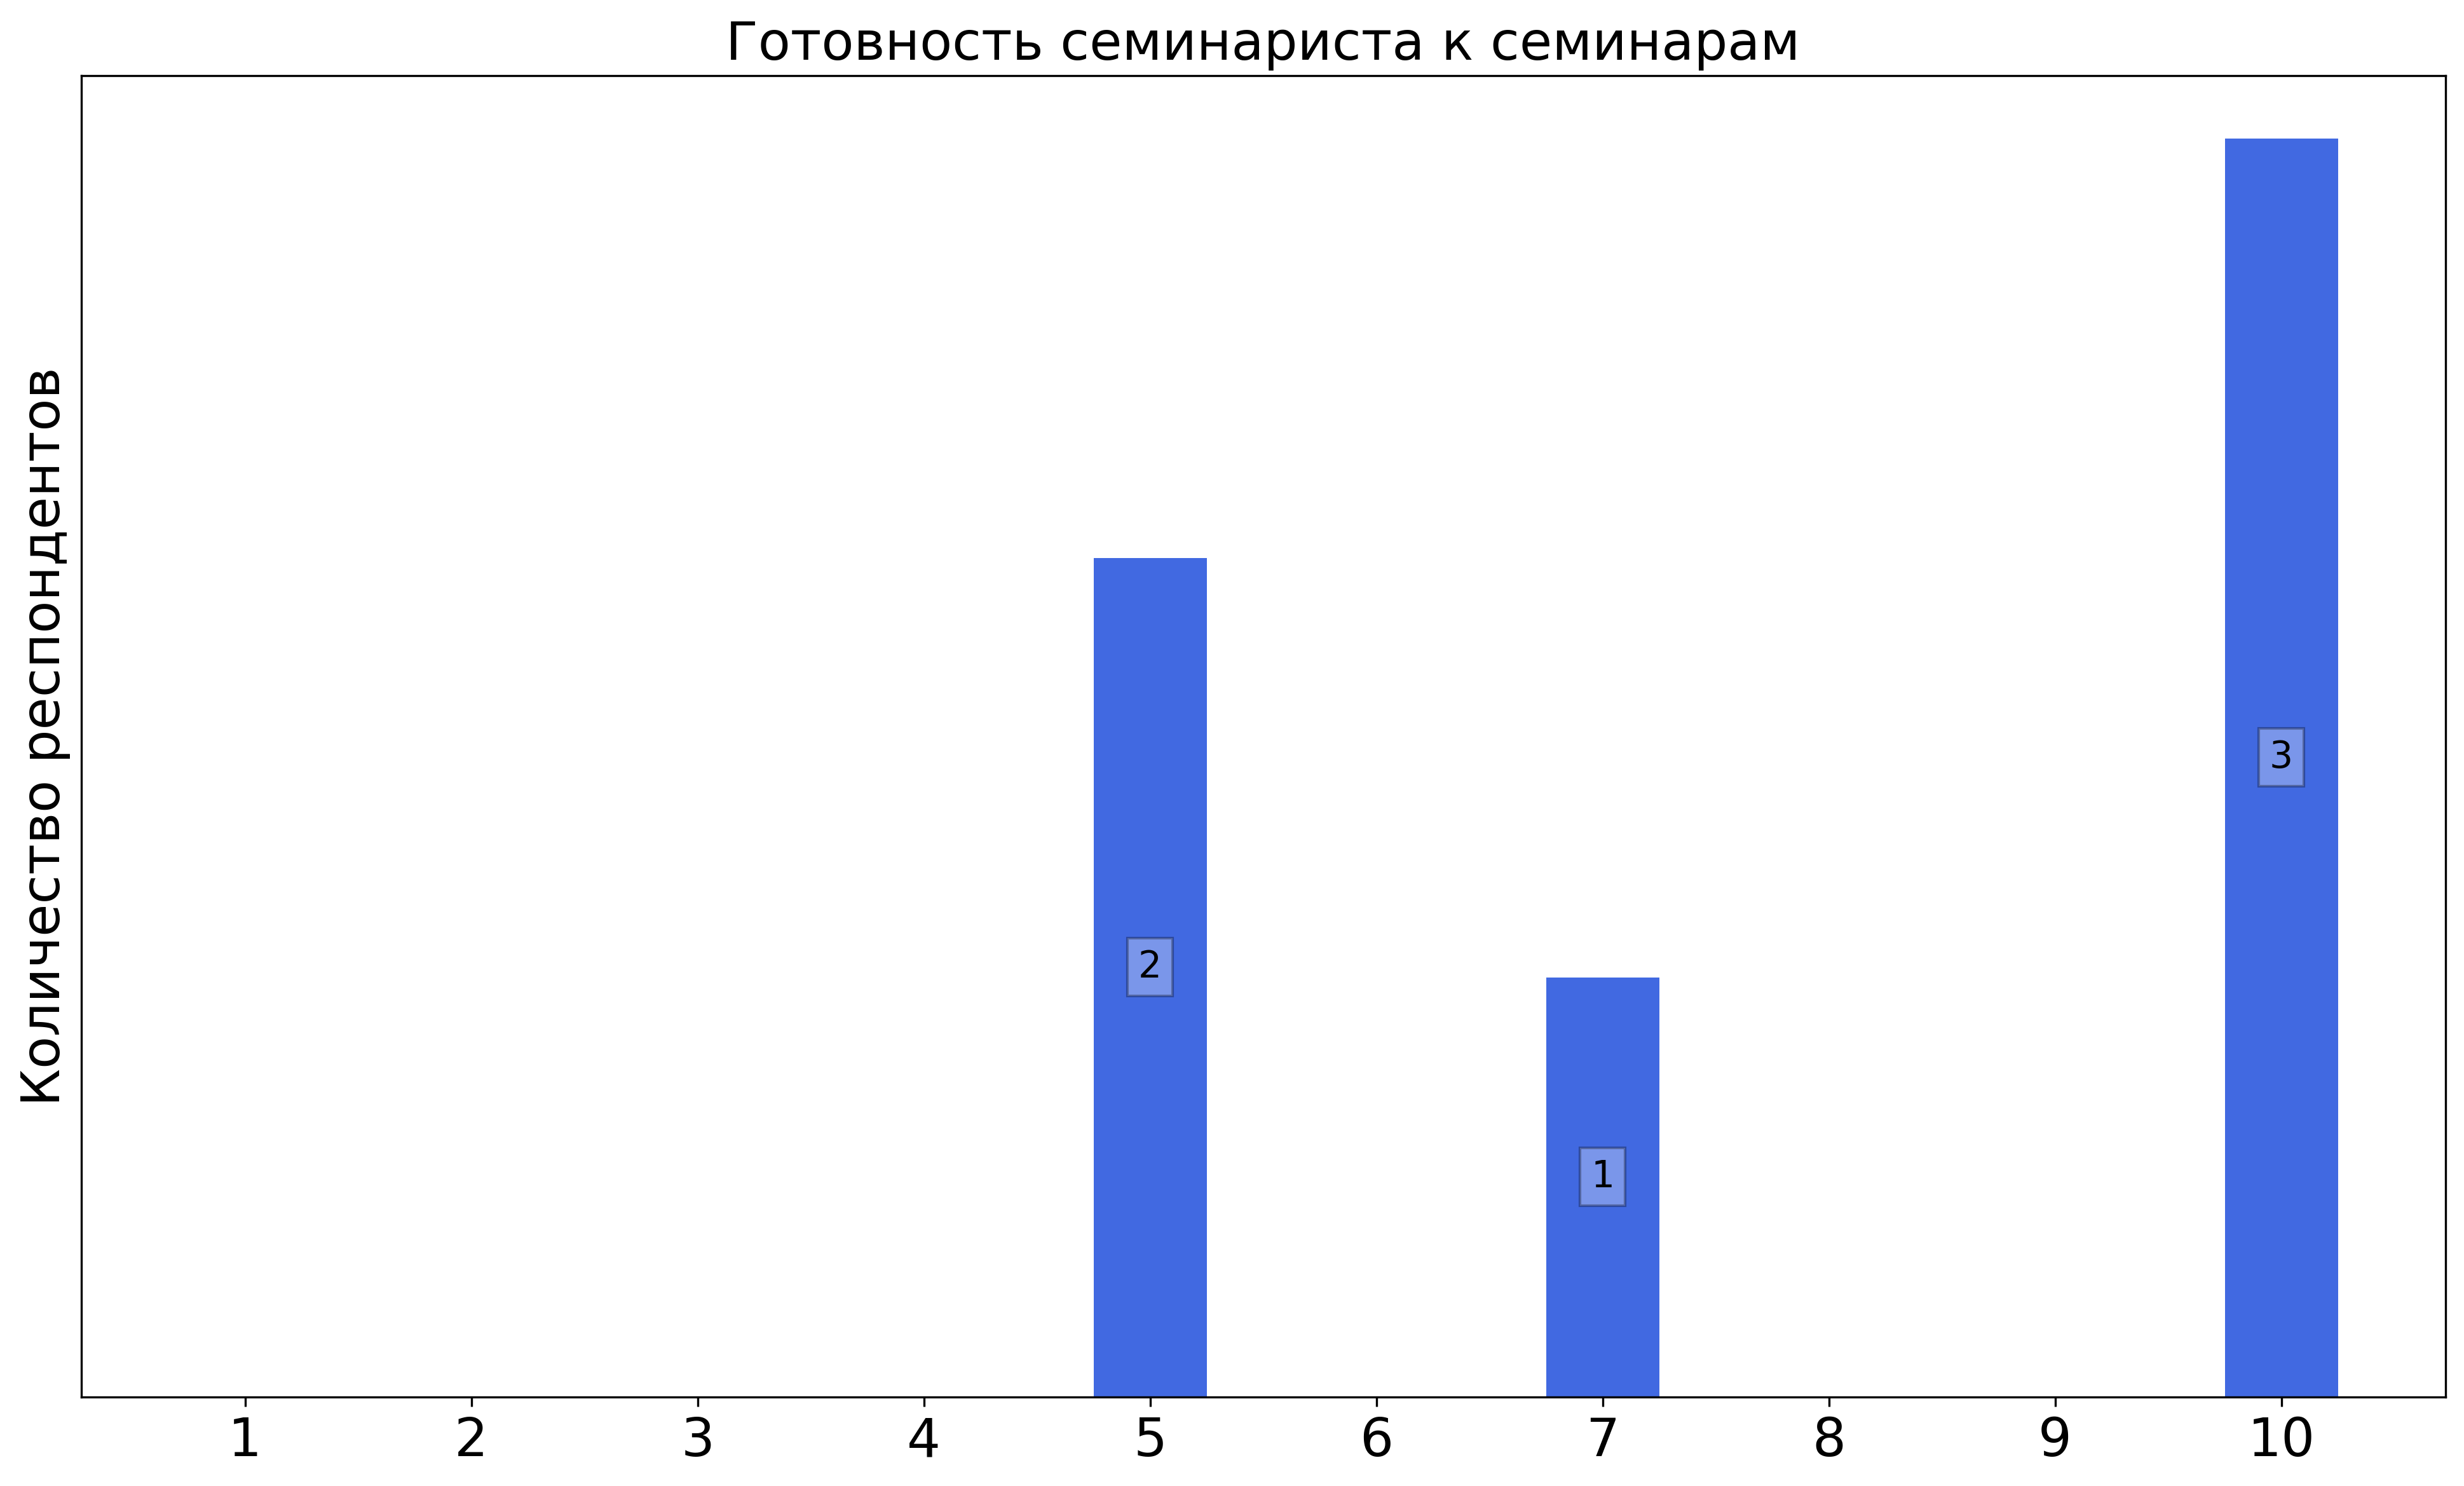
\includegraphics[width=\textwidth]{images/2 course/Аналитическая механика/seminarists-marks-Сидоренко В.В.-1.png}
            \end{subfigure}
            \begin{subfigure}[b]{0.45\textwidth}
                \centering
                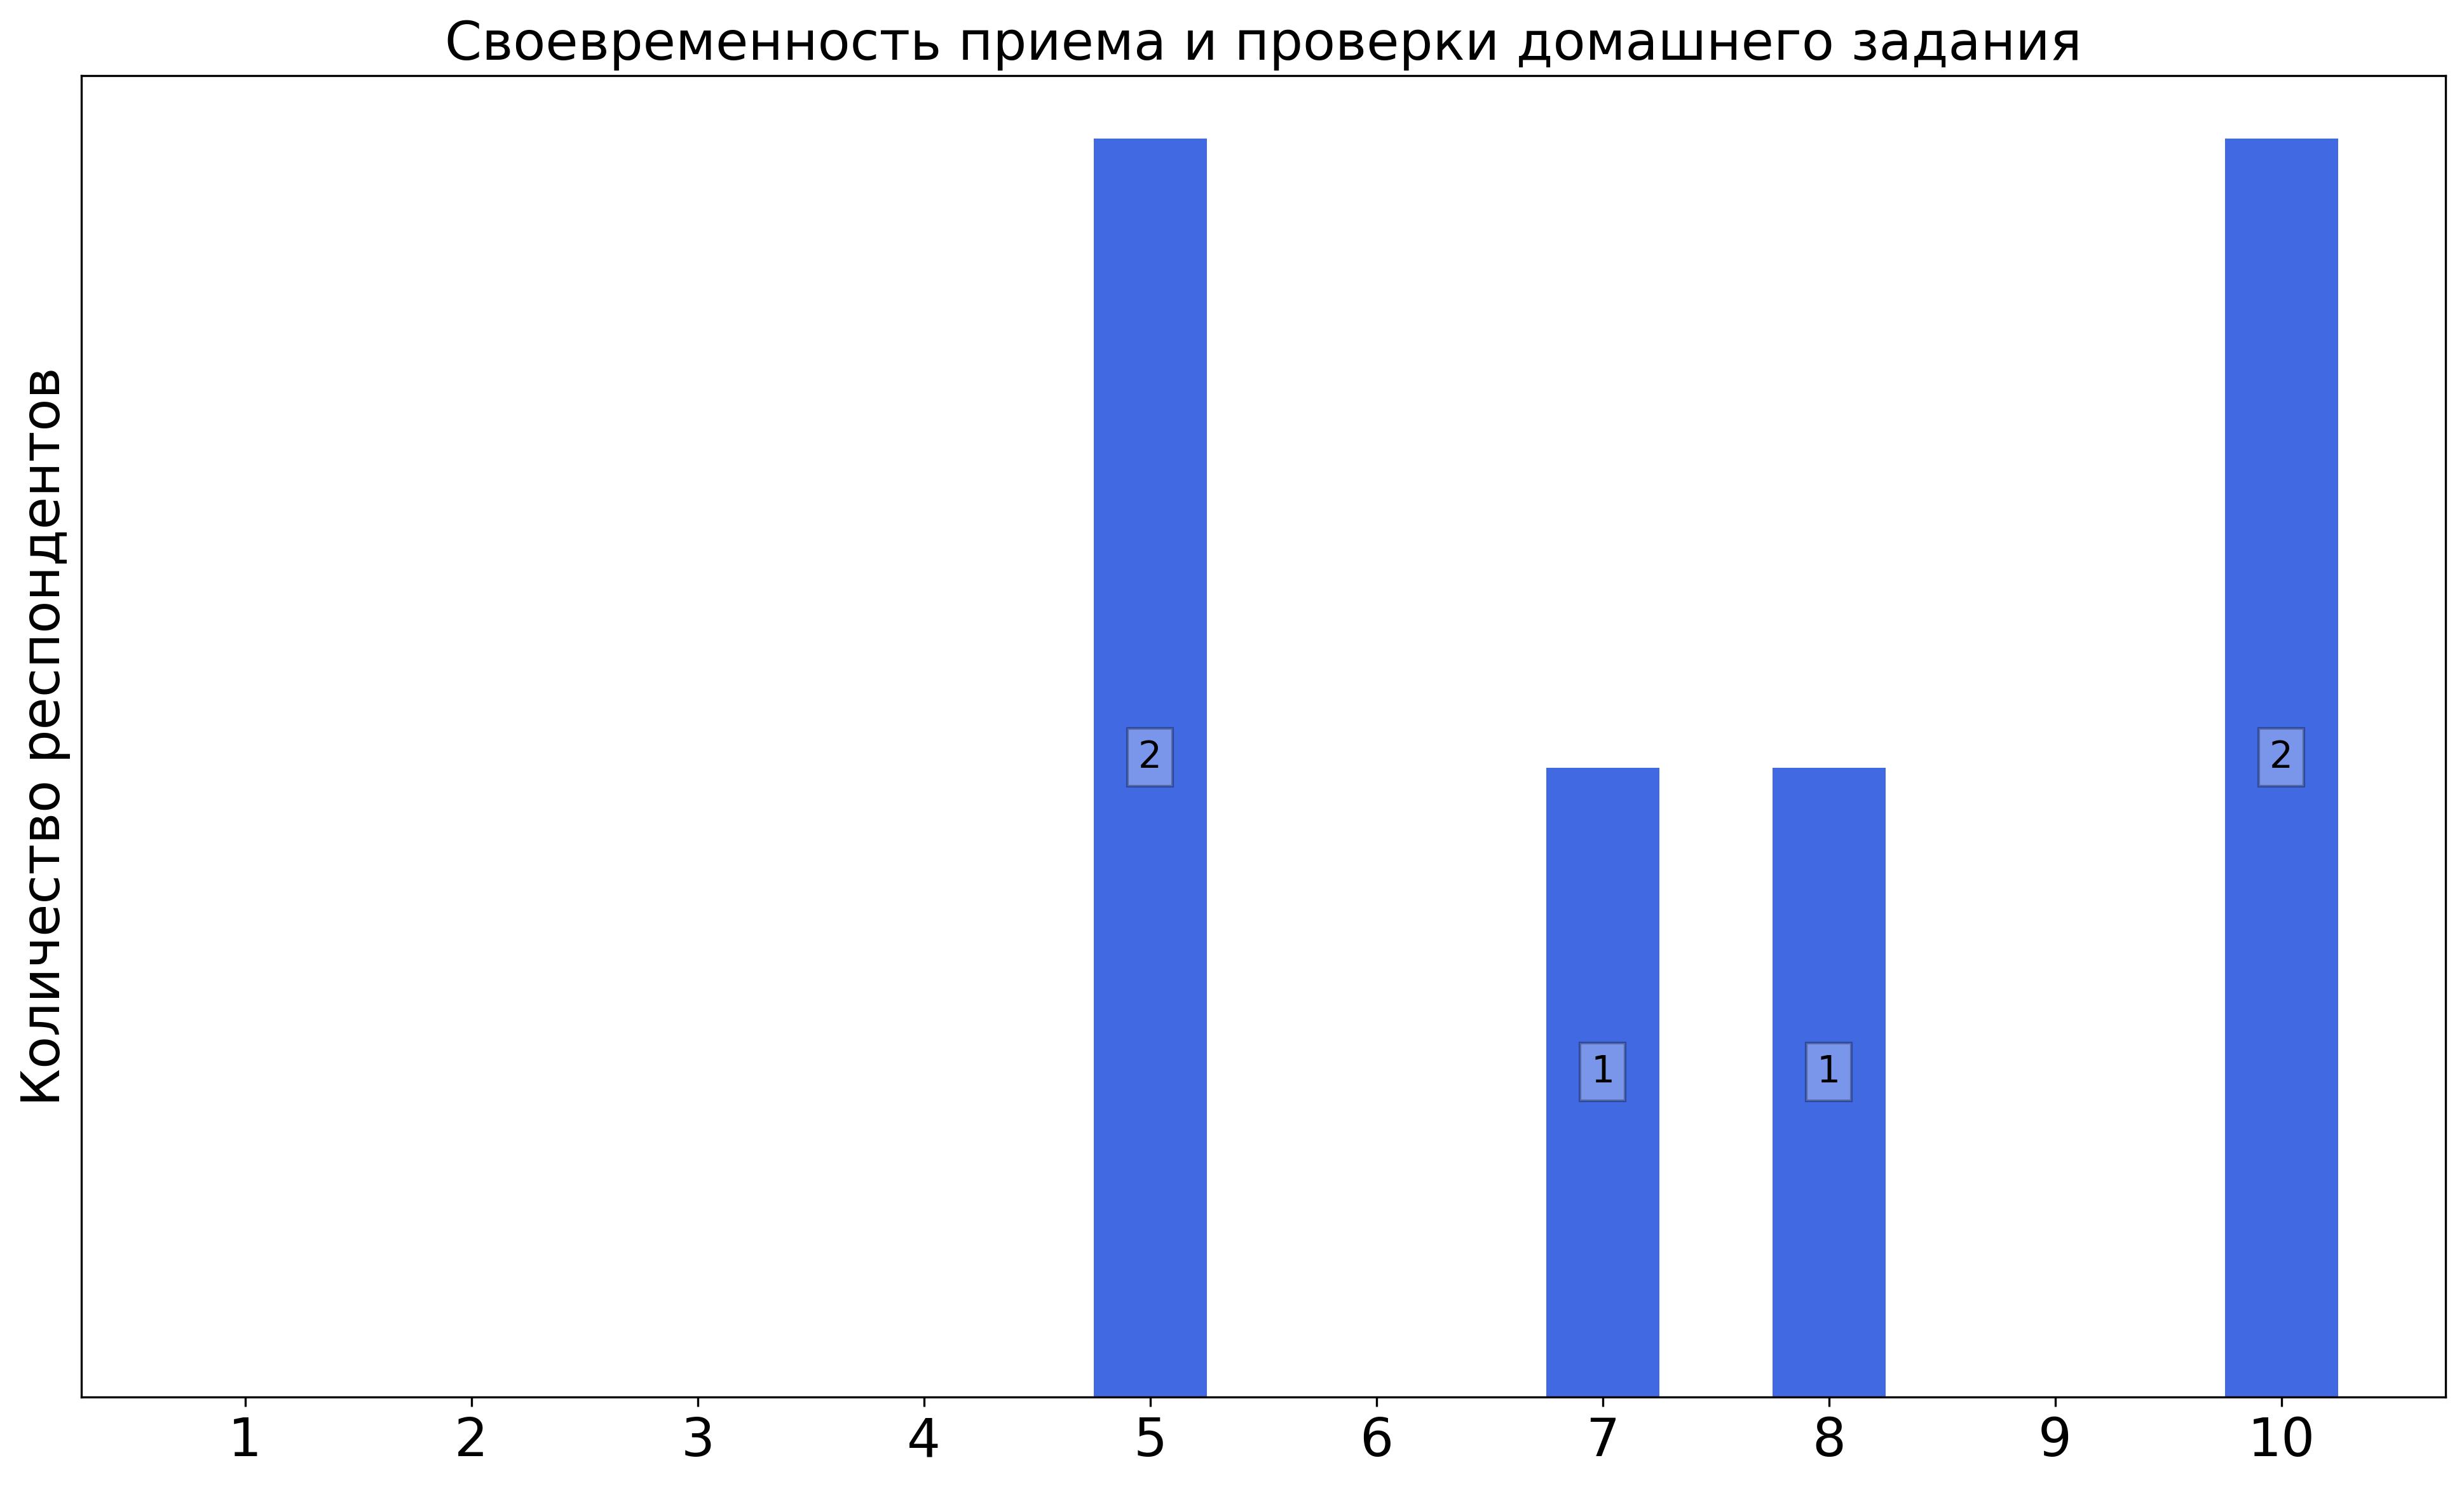
\includegraphics[width=\textwidth]{images/2 course/Аналитическая механика/seminarists-marks-Сидоренко В.В.-2.png}
            \end{subfigure}
            \begin{subfigure}[b]{0.45\textwidth}
                \centering
                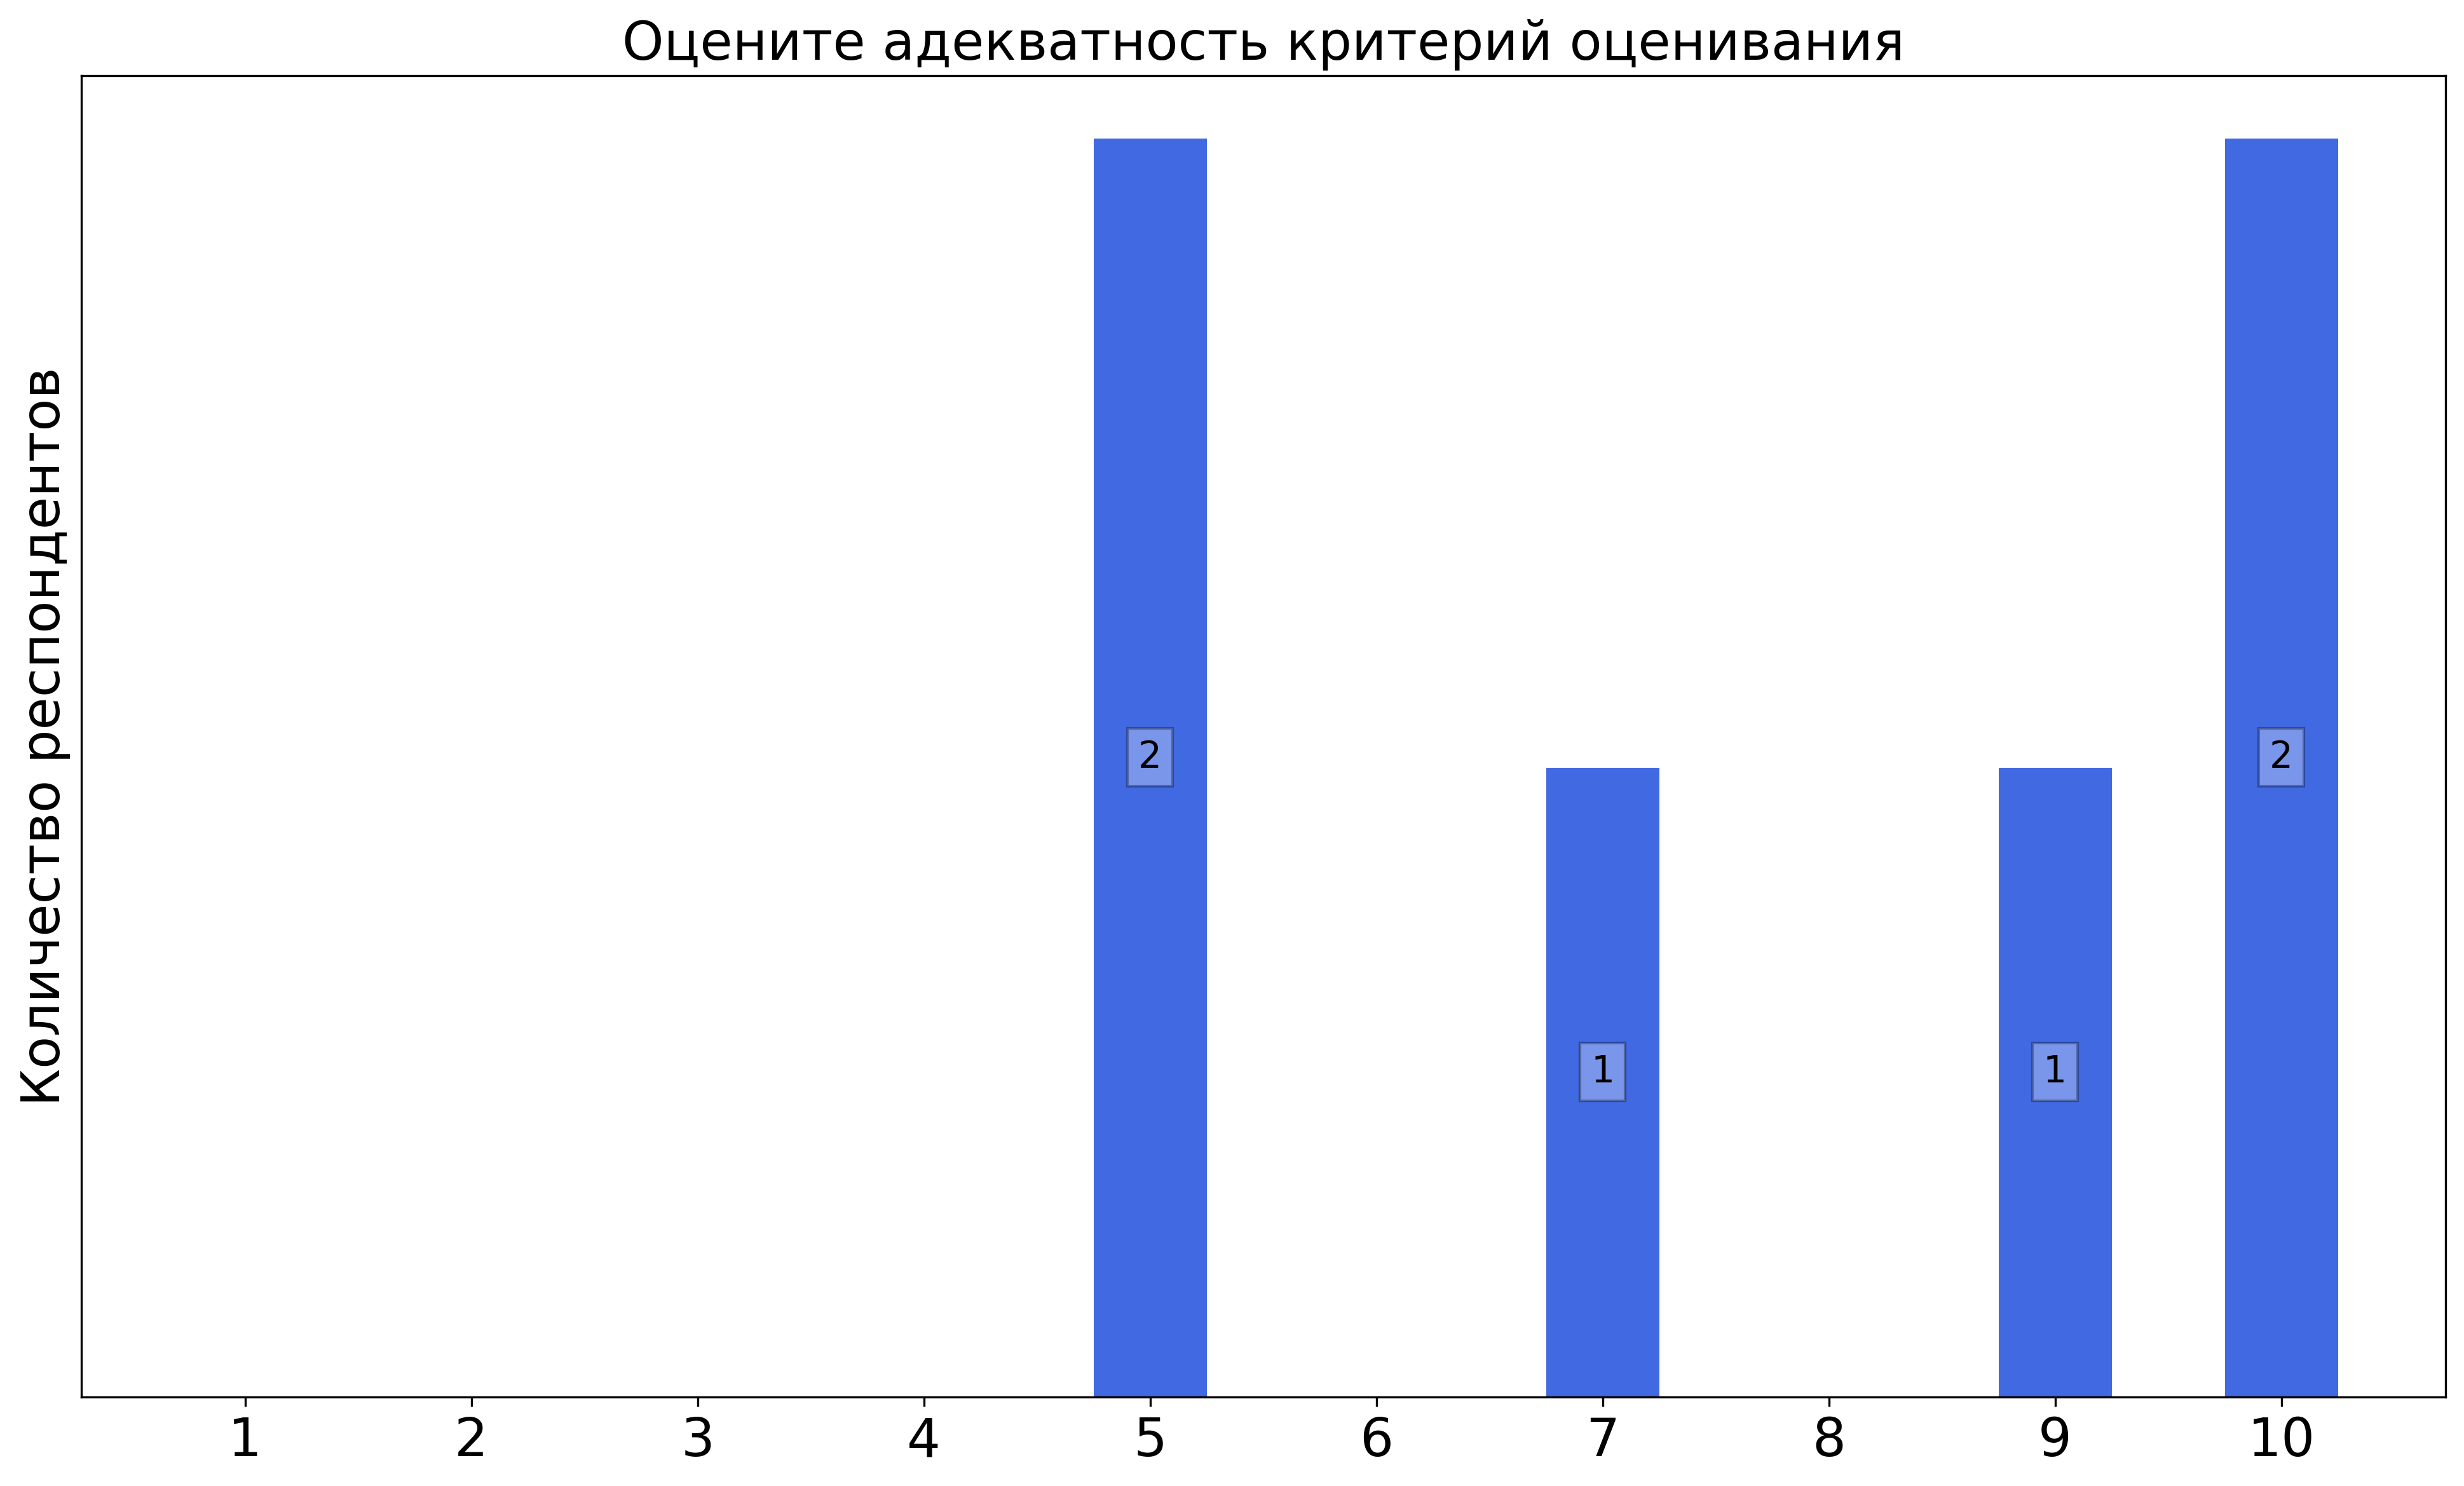
\includegraphics[width=\textwidth]{images/2 course/Аналитическая механика/seminarists-marks-Сидоренко В.В.-3.png}
            \end{subfigure}	
            \caption{Оценки респондентов о качестве преподавания семинаров}
        \end{figure}


    \subsubsection{Отзыв студентов о семинарах. Семинарист: Фомичев А.В.}
		\begin{figure}[H]
			\centering
			\begin{subfigure}[b]{0.45\textwidth}
				\centering
				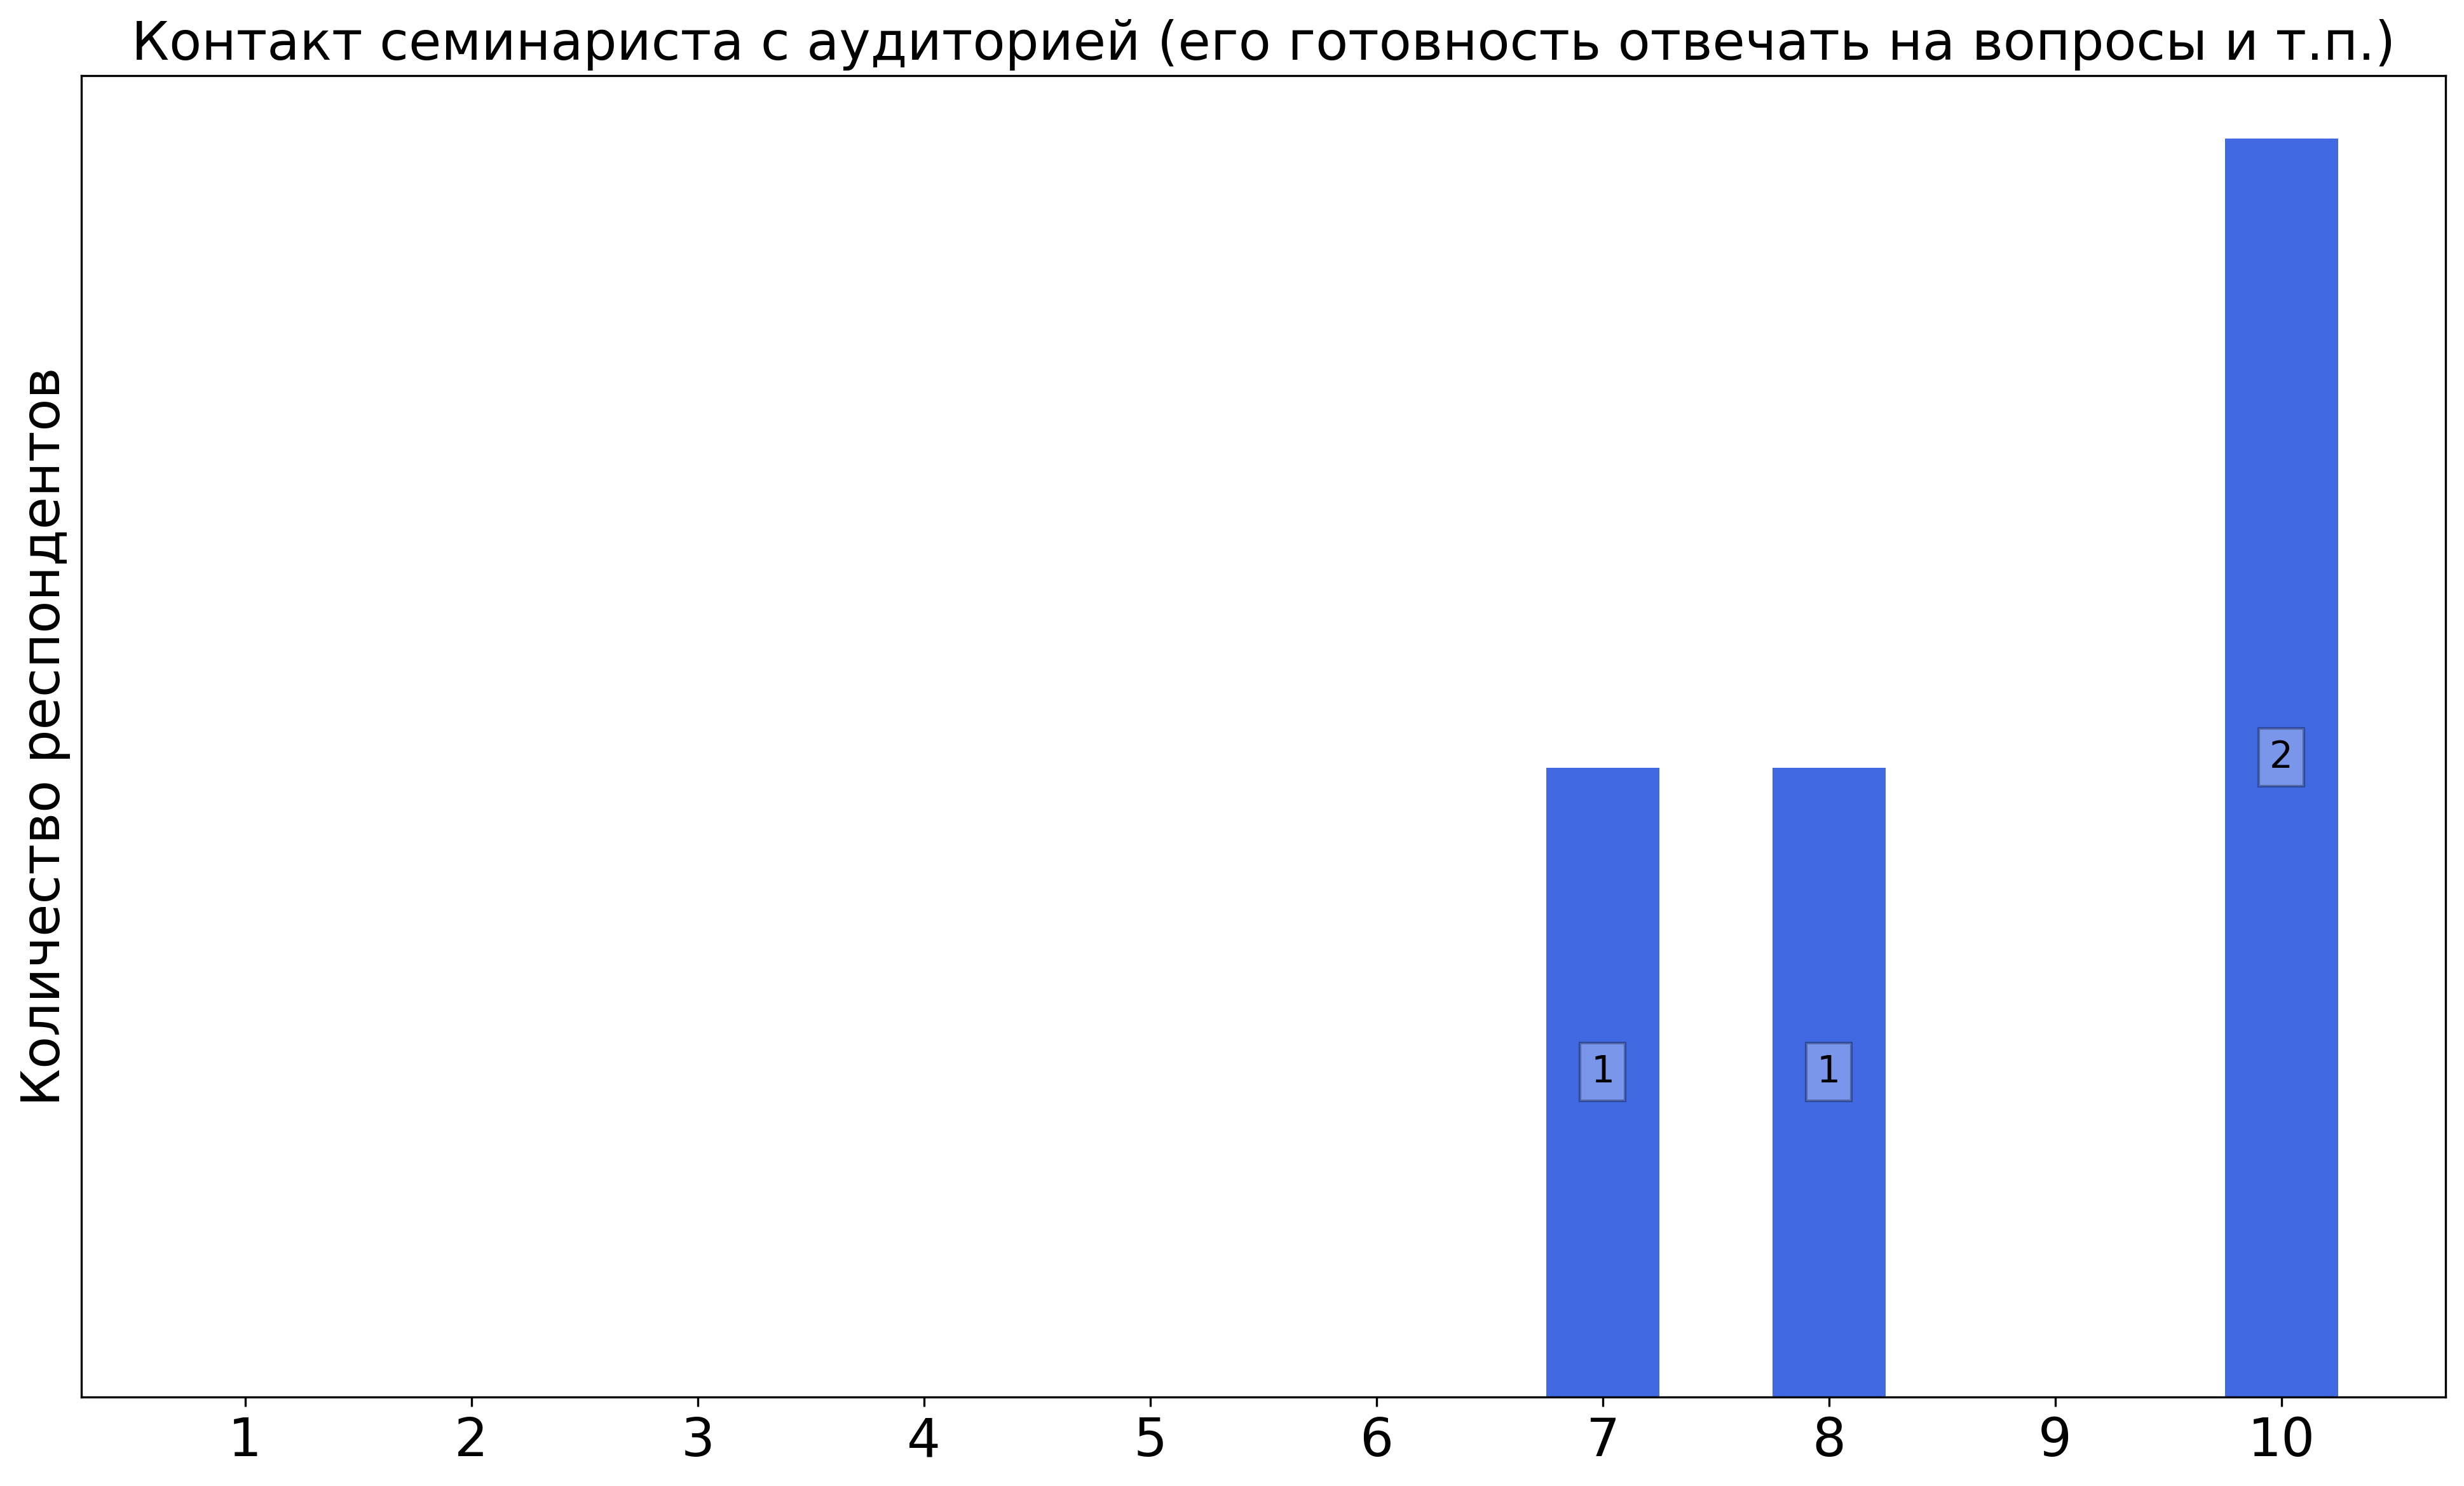
\includegraphics[width=\textwidth]{images/2 course/Аналитическая механика/seminarists-marks-Фомичев А.В.-0.png}
			\end{subfigure}
			\begin{subfigure}[b]{0.45\textwidth}
				\centering
				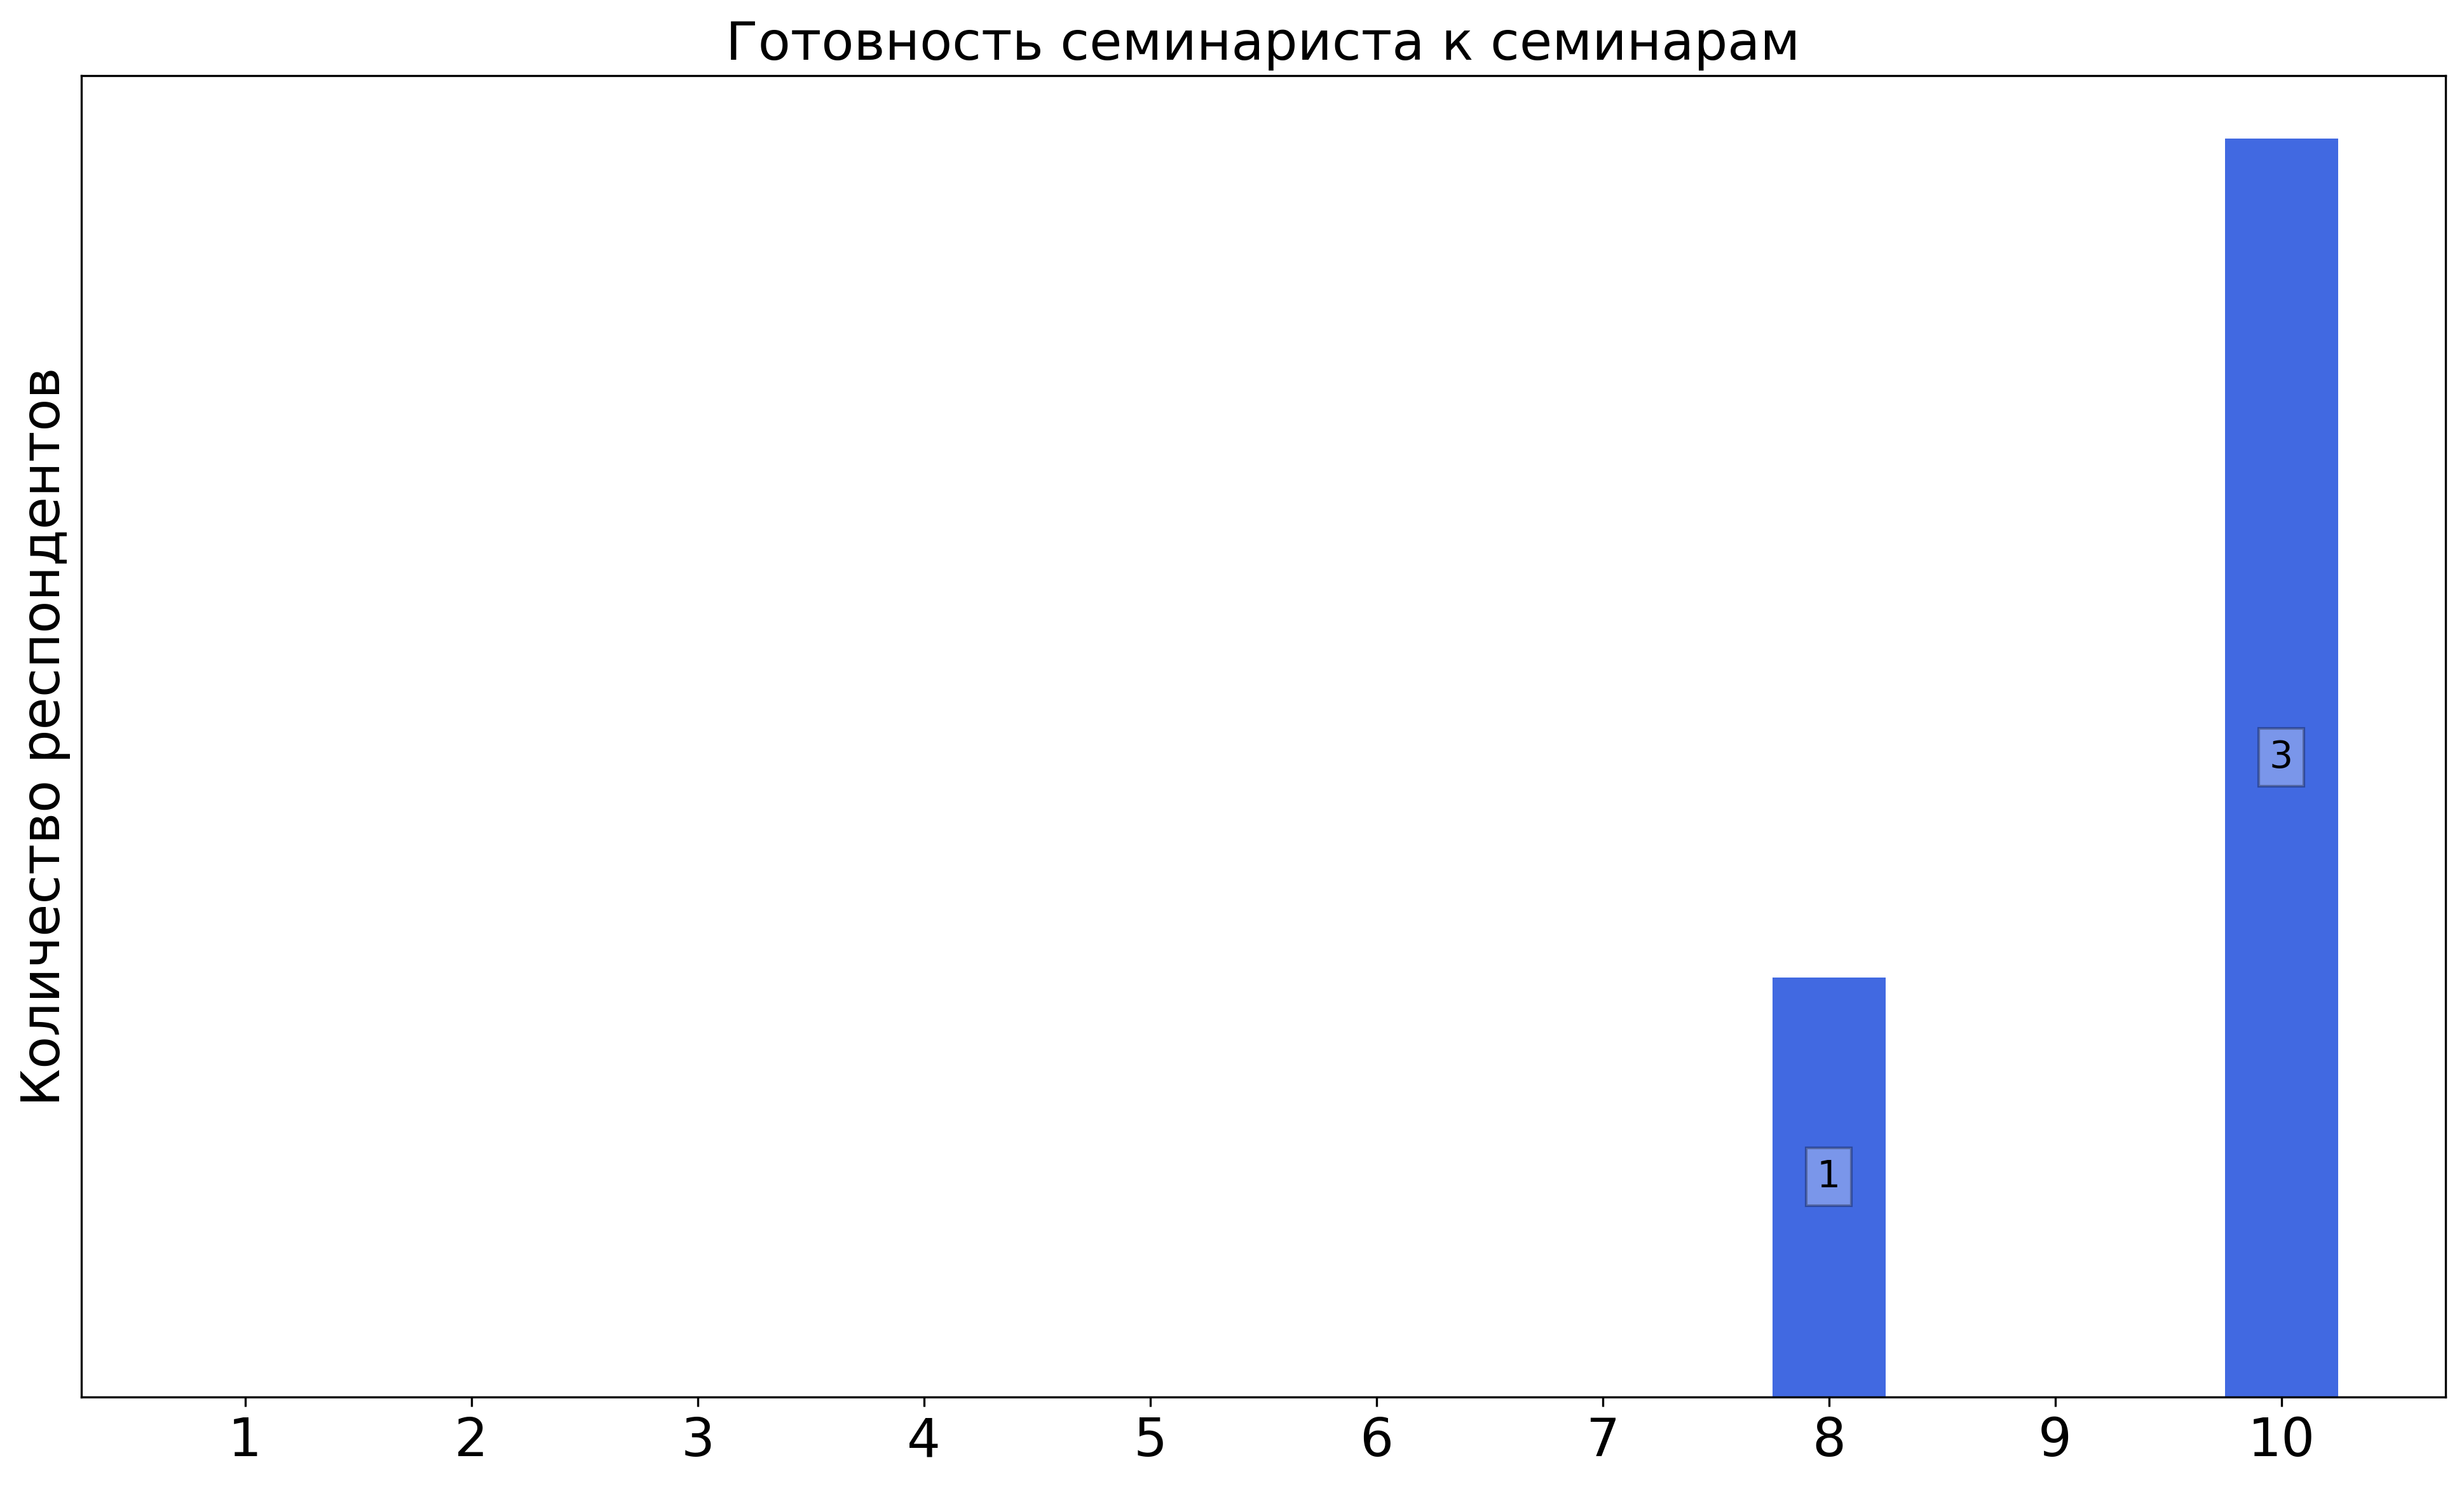
\includegraphics[width=\textwidth]{images/2 course/Аналитическая механика/seminarists-marks-Фомичев А.В.-1.png}
			\end{subfigure}
			\begin{subfigure}[b]{0.45\textwidth}
				\centering
				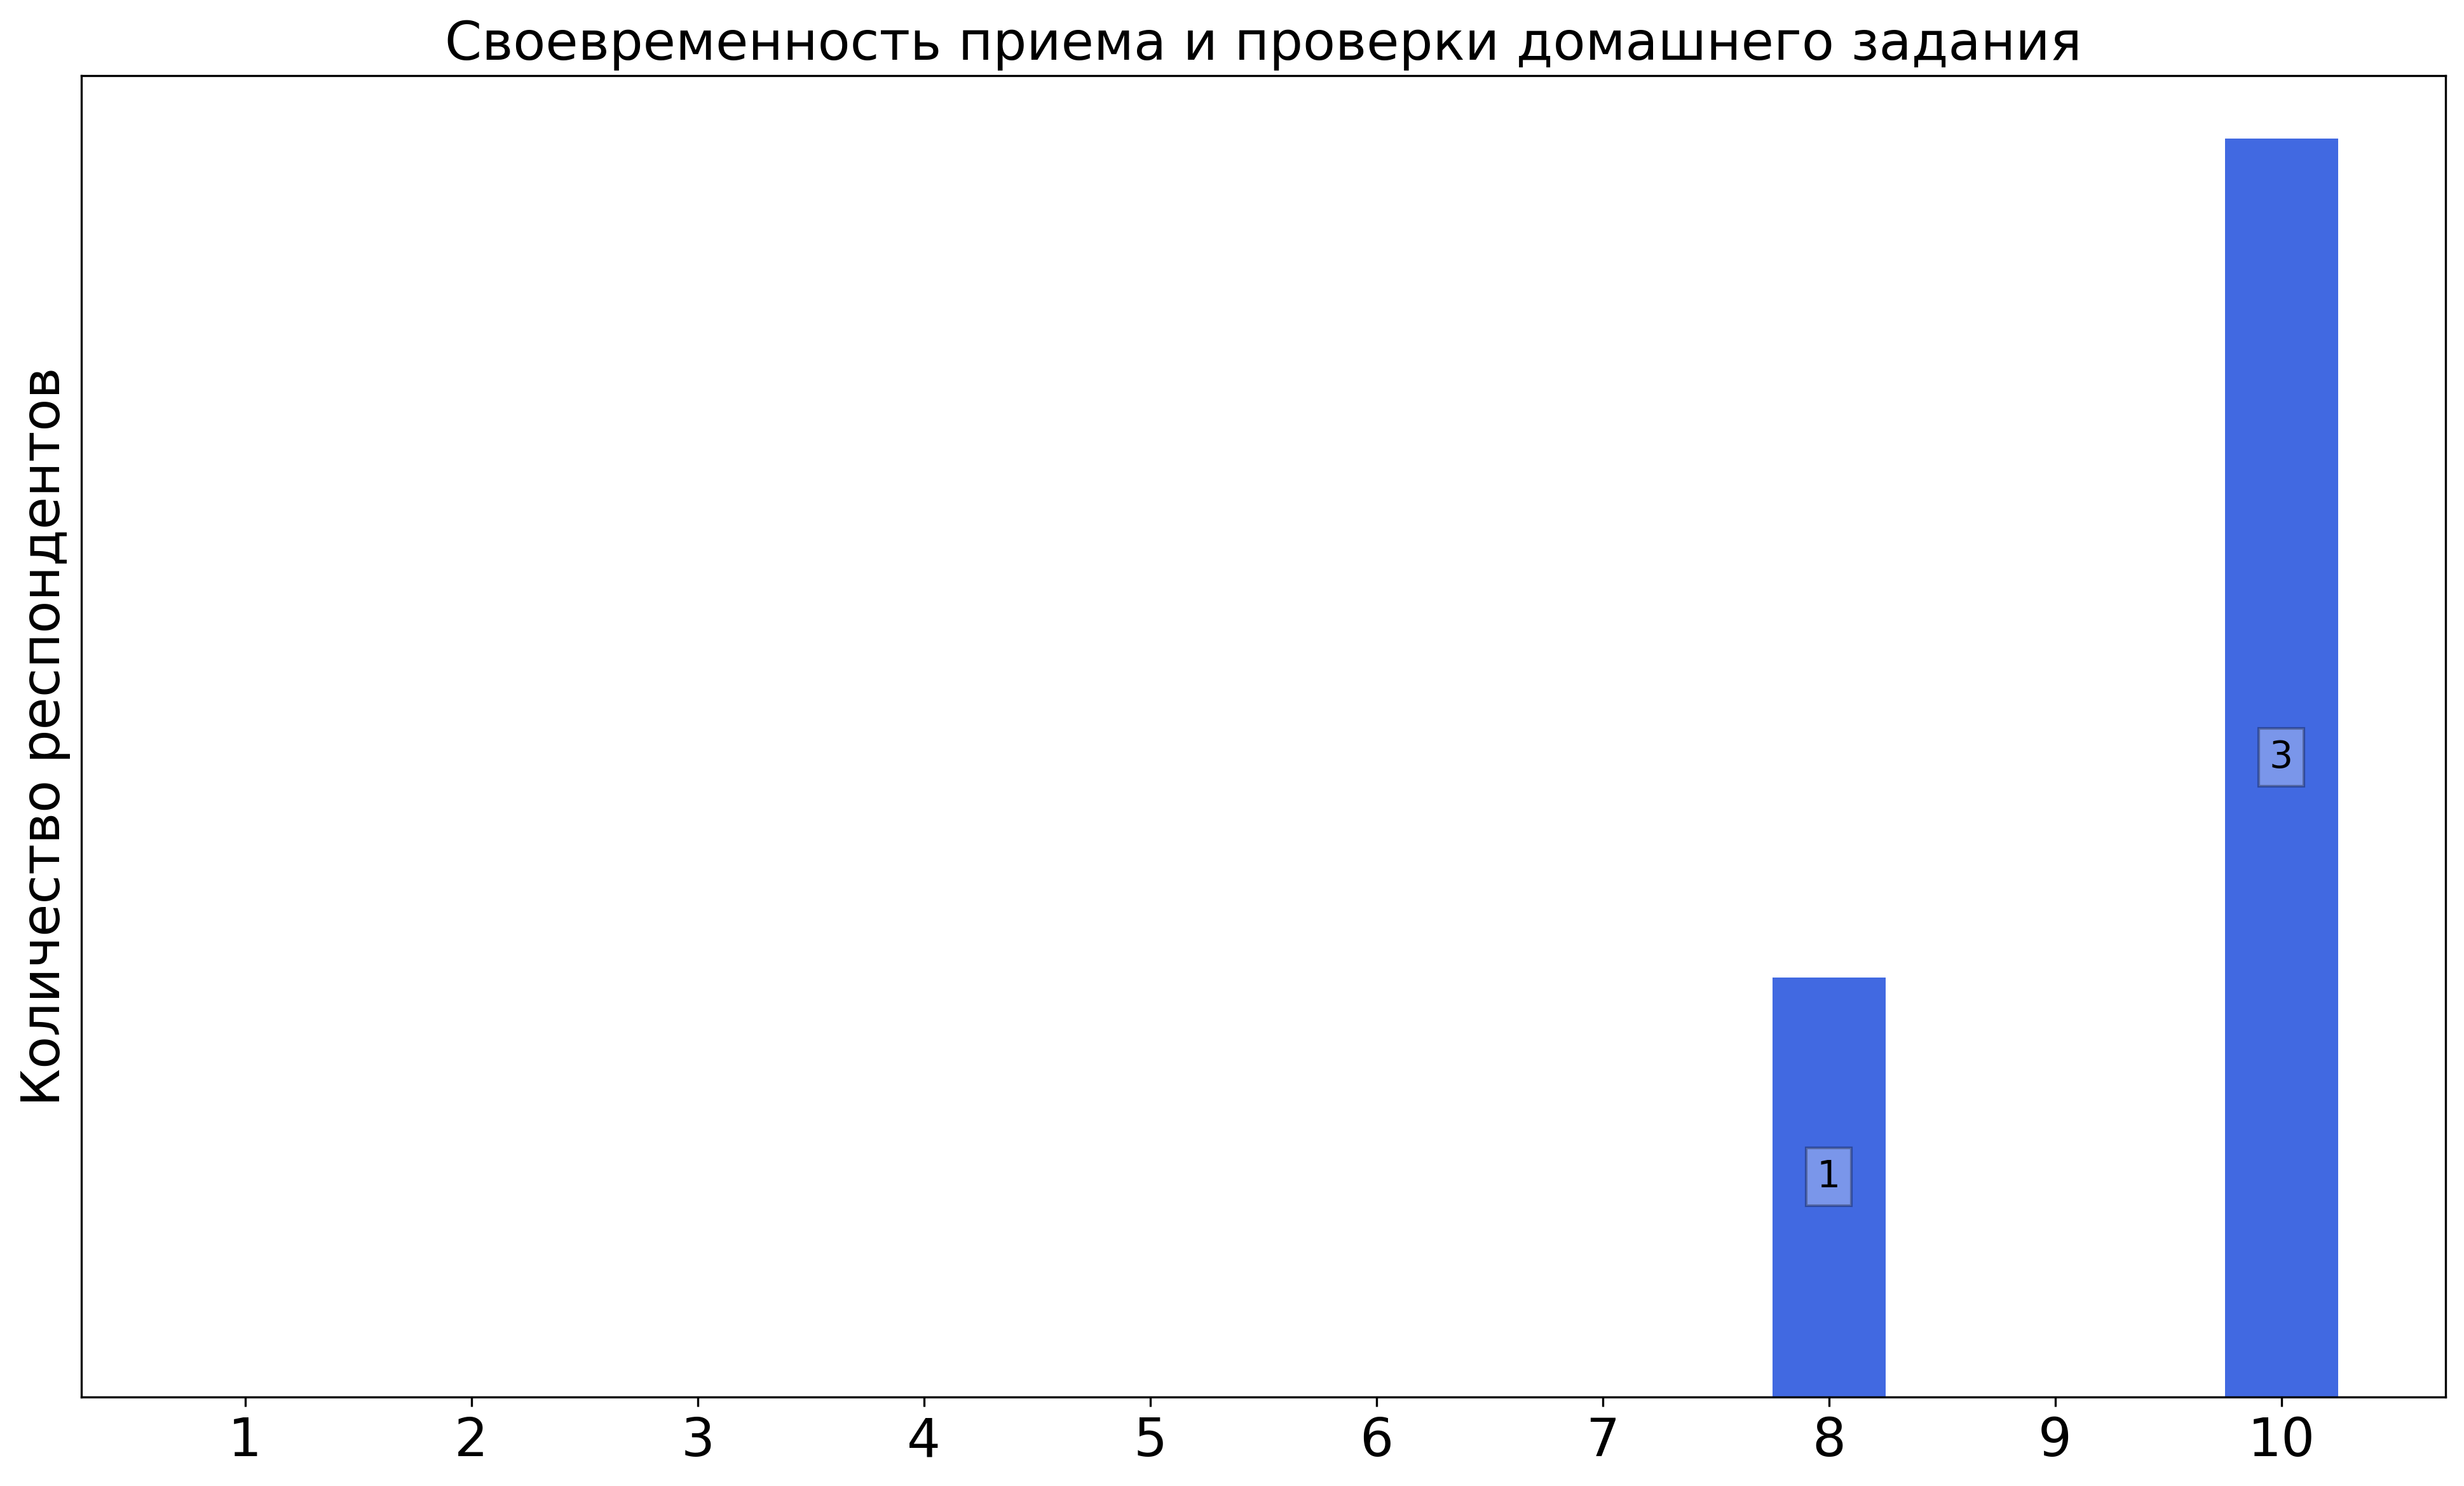
\includegraphics[width=\textwidth]{images/2 course/Аналитическая механика/seminarists-marks-Фомичев А.В.-2.png}
			\end{subfigure}
			\begin{subfigure}[b]{0.45\textwidth}
				\centering
				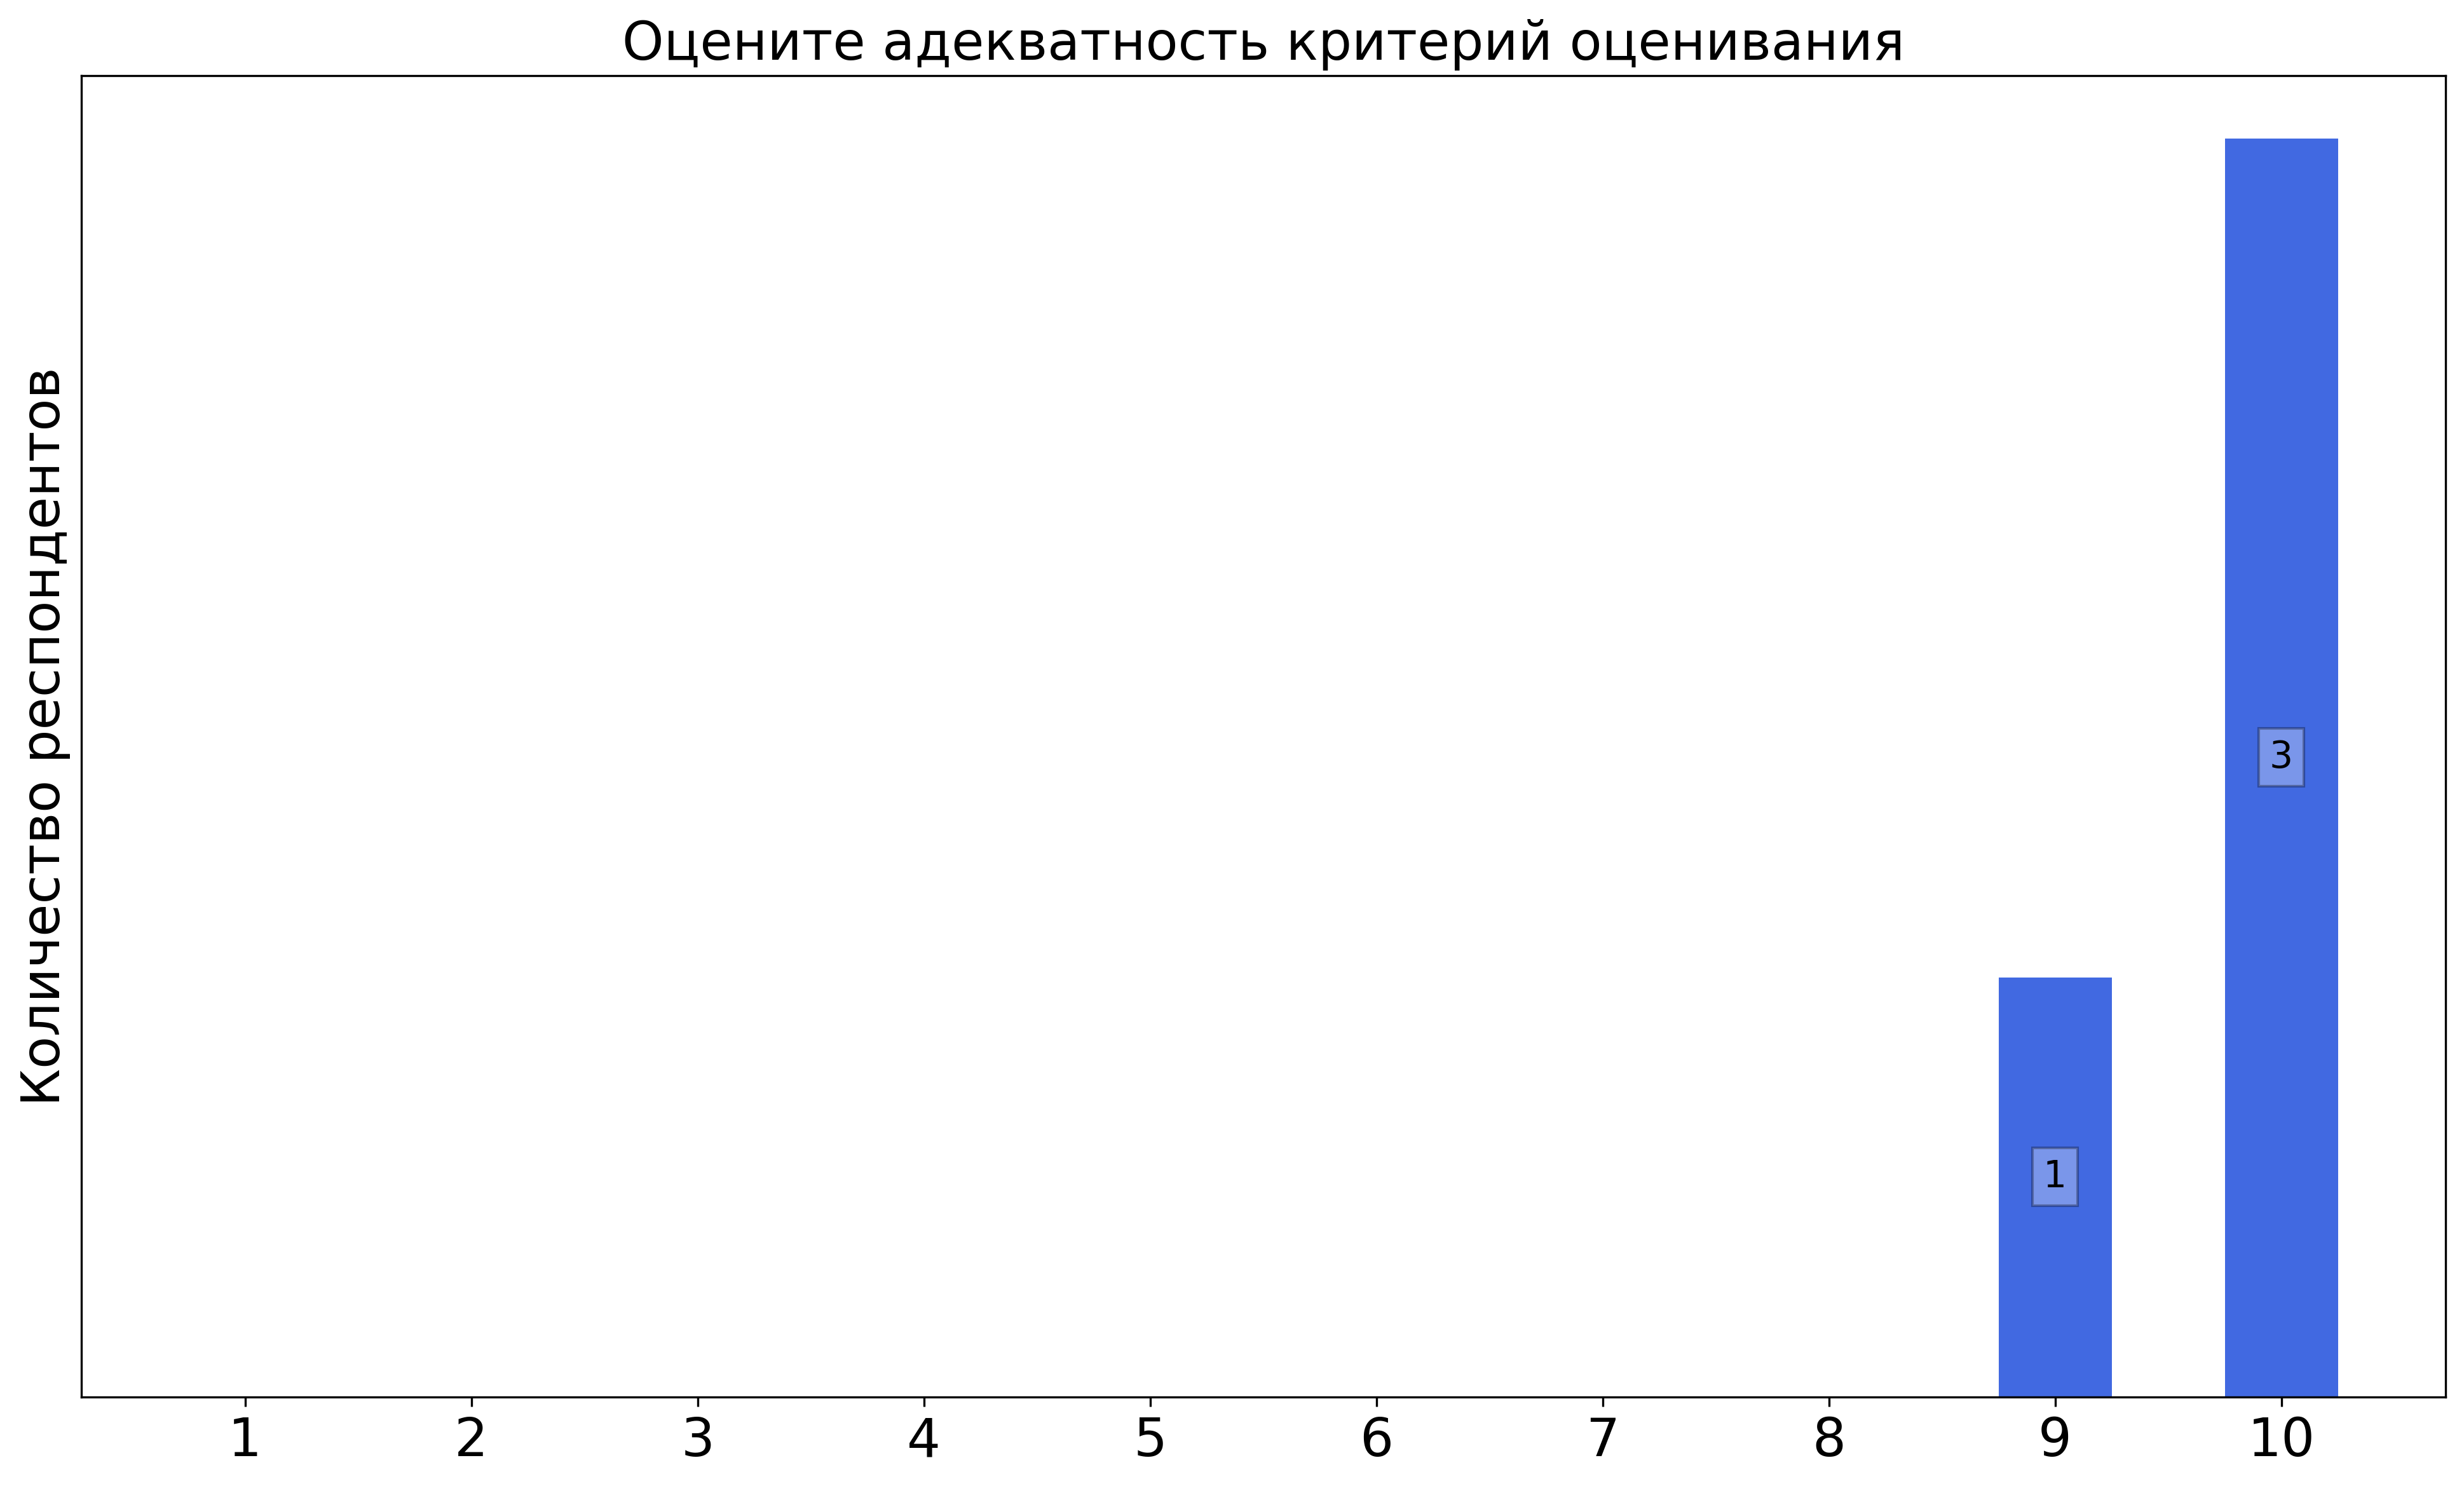
\includegraphics[width=\textwidth]{images/2 course/Аналитическая механика/seminarists-marks-Фомичев А.В.-3.png}
			\end{subfigure}	
			\caption{Оценки респондентов о качестве преподавания семинаров}
		\end{figure}

		\textbf{Комментарии студентов о семинаристе\protect\footnote{сохранены оригинальные орфография и пунктуация}}
            \begin{commentbox} 
                Хорошие семинары, правда местами ничего не понятно 
            \end{commentbox} 
